% Options for packages loaded elsewhere
\PassOptionsToPackage{unicode}{hyperref}
\PassOptionsToPackage{hyphens}{url}
%
\documentclass[
]{book}
\usepackage{lmodern}
\usepackage{amssymb,amsmath}
\usepackage{ifxetex,ifluatex}
\ifnum 0\ifxetex 1\fi\ifluatex 1\fi=0 % if pdftex
  \usepackage[T1]{fontenc}
  \usepackage[utf8]{inputenc}
  \usepackage{textcomp} % provide euro and other symbols
\else % if luatex or xetex
  \usepackage{unicode-math}
  \defaultfontfeatures{Scale=MatchLowercase}
  \defaultfontfeatures[\rmfamily]{Ligatures=TeX,Scale=1}
\fi
% Use upquote if available, for straight quotes in verbatim environments
\IfFileExists{upquote.sty}{\usepackage{upquote}}{}
\IfFileExists{microtype.sty}{% use microtype if available
  \usepackage[]{microtype}
  \UseMicrotypeSet[protrusion]{basicmath} % disable protrusion for tt fonts
}{}
\makeatletter
\@ifundefined{KOMAClassName}{% if non-KOMA class
  \IfFileExists{parskip.sty}{%
    \usepackage{parskip}
  }{% else
    \setlength{\parindent}{0pt}
    \setlength{\parskip}{6pt plus 2pt minus 1pt}}
}{% if KOMA class
  \KOMAoptions{parskip=half}}
\makeatother
\usepackage{xcolor}
\IfFileExists{xurl.sty}{\usepackage{xurl}}{} % add URL line breaks if available
\IfFileExists{bookmark.sty}{\usepackage{bookmark}}{\usepackage{hyperref}}
\hypersetup{
  pdftitle={Data Science for Biological, Medical and Health Research: Notes for PQHS/CRSP/MPHP 431},
  pdfauthor={Thomas E. Love},
  hidelinks,
  pdfcreator={LaTeX via pandoc}}
\urlstyle{same} % disable monospaced font for URLs
\usepackage{color}
\usepackage{fancyvrb}
\newcommand{\VerbBar}{|}
\newcommand{\VERB}{\Verb[commandchars=\\\{\}]}
\DefineVerbatimEnvironment{Highlighting}{Verbatim}{commandchars=\\\{\}}
% Add ',fontsize=\small' for more characters per line
\usepackage{framed}
\definecolor{shadecolor}{RGB}{248,248,248}
\newenvironment{Shaded}{\begin{snugshade}}{\end{snugshade}}
\newcommand{\AlertTok}[1]{\textcolor[rgb]{0.94,0.16,0.16}{#1}}
\newcommand{\AnnotationTok}[1]{\textcolor[rgb]{0.56,0.35,0.01}{\textbf{\textit{#1}}}}
\newcommand{\AttributeTok}[1]{\textcolor[rgb]{0.77,0.63,0.00}{#1}}
\newcommand{\BaseNTok}[1]{\textcolor[rgb]{0.00,0.00,0.81}{#1}}
\newcommand{\BuiltInTok}[1]{#1}
\newcommand{\CharTok}[1]{\textcolor[rgb]{0.31,0.60,0.02}{#1}}
\newcommand{\CommentTok}[1]{\textcolor[rgb]{0.56,0.35,0.01}{\textit{#1}}}
\newcommand{\CommentVarTok}[1]{\textcolor[rgb]{0.56,0.35,0.01}{\textbf{\textit{#1}}}}
\newcommand{\ConstantTok}[1]{\textcolor[rgb]{0.00,0.00,0.00}{#1}}
\newcommand{\ControlFlowTok}[1]{\textcolor[rgb]{0.13,0.29,0.53}{\textbf{#1}}}
\newcommand{\DataTypeTok}[1]{\textcolor[rgb]{0.13,0.29,0.53}{#1}}
\newcommand{\DecValTok}[1]{\textcolor[rgb]{0.00,0.00,0.81}{#1}}
\newcommand{\DocumentationTok}[1]{\textcolor[rgb]{0.56,0.35,0.01}{\textbf{\textit{#1}}}}
\newcommand{\ErrorTok}[1]{\textcolor[rgb]{0.64,0.00,0.00}{\textbf{#1}}}
\newcommand{\ExtensionTok}[1]{#1}
\newcommand{\FloatTok}[1]{\textcolor[rgb]{0.00,0.00,0.81}{#1}}
\newcommand{\FunctionTok}[1]{\textcolor[rgb]{0.00,0.00,0.00}{#1}}
\newcommand{\ImportTok}[1]{#1}
\newcommand{\InformationTok}[1]{\textcolor[rgb]{0.56,0.35,0.01}{\textbf{\textit{#1}}}}
\newcommand{\KeywordTok}[1]{\textcolor[rgb]{0.13,0.29,0.53}{\textbf{#1}}}
\newcommand{\NormalTok}[1]{#1}
\newcommand{\OperatorTok}[1]{\textcolor[rgb]{0.81,0.36,0.00}{\textbf{#1}}}
\newcommand{\OtherTok}[1]{\textcolor[rgb]{0.56,0.35,0.01}{#1}}
\newcommand{\PreprocessorTok}[1]{\textcolor[rgb]{0.56,0.35,0.01}{\textit{#1}}}
\newcommand{\RegionMarkerTok}[1]{#1}
\newcommand{\SpecialCharTok}[1]{\textcolor[rgb]{0.00,0.00,0.00}{#1}}
\newcommand{\SpecialStringTok}[1]{\textcolor[rgb]{0.31,0.60,0.02}{#1}}
\newcommand{\StringTok}[1]{\textcolor[rgb]{0.31,0.60,0.02}{#1}}
\newcommand{\VariableTok}[1]{\textcolor[rgb]{0.00,0.00,0.00}{#1}}
\newcommand{\VerbatimStringTok}[1]{\textcolor[rgb]{0.31,0.60,0.02}{#1}}
\newcommand{\WarningTok}[1]{\textcolor[rgb]{0.56,0.35,0.01}{\textbf{\textit{#1}}}}
\usepackage{longtable,booktabs}
% Correct order of tables after \paragraph or \subparagraph
\usepackage{etoolbox}
\makeatletter
\patchcmd\longtable{\par}{\if@noskipsec\mbox{}\fi\par}{}{}
\makeatother
% Allow footnotes in longtable head/foot
\IfFileExists{footnotehyper.sty}{\usepackage{footnotehyper}}{\usepackage{footnote}}
\makesavenoteenv{longtable}
\usepackage{graphicx,grffile}
\makeatletter
\def\maxwidth{\ifdim\Gin@nat@width>\linewidth\linewidth\else\Gin@nat@width\fi}
\def\maxheight{\ifdim\Gin@nat@height>\textheight\textheight\else\Gin@nat@height\fi}
\makeatother
% Scale images if necessary, so that they will not overflow the page
% margins by default, and it is still possible to overwrite the defaults
% using explicit options in \includegraphics[width, height, ...]{}
\setkeys{Gin}{width=\maxwidth,height=\maxheight,keepaspectratio}
% Set default figure placement to htbp
\makeatletter
\def\fps@figure{htbp}
\makeatother
\setlength{\emergencystretch}{3em} % prevent overfull lines
\providecommand{\tightlist}{%
  \setlength{\itemsep}{0pt}\setlength{\parskip}{0pt}}
\setcounter{secnumdepth}{5}
\usepackage{booktabs}
\usepackage{amsthm}
\makeatletter
\def\thm@space@setup{%
  \thm@preskip=8pt plus 2pt minus 4pt
  \thm@postskip=\thm@preskip
}
\makeatother
\usepackage[]{natbib}
\bibliographystyle{apalike}

\title{Data Science for Biological, Medical and Health Research: Notes for PQHS/CRSP/MPHP 431}
\author{Thomas E. Love}
\date{2020-08-24}

\begin{document}
\maketitle

{
\setcounter{tocdepth}{1}
\tableofcontents
}
\hypertarget{working-with-these-notes}{%
\chapter*{Working with These Notes}\label{working-with-these-notes}}
\addcontentsline{toc}{chapter}{Working with These Notes}

\begin{enumerate}
\def\labelenumi{\arabic{enumi}.}
\tightlist
\item
  This document is broken down into multiple chapters. Use the table of contents on the left side of the screen to navigate, and use the hamburger icon (horizontal bars) at the top of the document to open or close the table of contents.
\item
  At the top of the document, you'll see additional icons which you can click to

  \begin{itemize}
  \tightlist
  \item
    search the document,
  \item
    change the size, font or color scheme of the page, and
  \item
    download a PDF or EPUB (Kindle-readable) version of the entire document.
  \end{itemize}
\item
  The document will be updated (unpredictably) throughout the semester.
\end{enumerate}

\hypertarget{the-431-course-online}{%
\section*{The 431 Course online}\label{the-431-course-online}}
\addcontentsline{toc}{section}{The 431 Course online}

The \textbf{main web page} for the 431 course in Fall 2020 is \url{https://thomaselove.github.io/431/}. Go there for all information related to the course.

\hypertarget{what-youll-find-here}{%
\section*{What You'll Find Here}\label{what-youll-find-here}}
\addcontentsline{toc}{section}{What You'll Find Here}

These Notes provide a series of examples using R to work through issues that are likely to come up in PQHS/CRSP/MPHP 431. What you will mostly find are brief explanations of a key idea or summary, accompanied (most of the time) by R code and a demonstration of the results of applying that code.

While these Notes share some of the features of a textbook, they are neither comprehensive nor completely original. The main purpose is to give 431 students a set of common materials on which to draw during the course. In class, we will sometimes:

\begin{itemize}
\tightlist
\item
  reiterate points made in this document,
\item
  amplify what is here,
\item
  simplify the presentation of things done here,
\item
  use new examples to show some of the same techniques,
\item
  refer to issues not mentioned in this document,
\end{itemize}

but what we don't do is follow these notes very precisely. We assume instead that you will read the materials and try to learn from them, just as you will attend classes and try to learn from them. We welcome feedback of all kinds on this document or anything else.

Everything you see here is available to you as HTML or PDF. You will also have access to the R Markdown files, which contain the code which generates everything in the document, including all of the R results. We will demonstrate the use of R Markdown (this document is generated with the additional help of an R package called \texttt{bookdown}) and RStudio (the ``program'' we use to interface with the R language) in class.

All data and R code related to these notes are also available to you.

\hypertarget{setting-up-r}{%
\section*{Setting Up R}\label{setting-up-r}}
\addcontentsline{toc}{section}{Setting Up R}

These Notes make extensive use of

\begin{itemize}
\tightlist
\item
  the statistical software language R, and
\item
  the development environment R Studio,
\end{itemize}

both of which are free, and you'll need to install them on your machine. Instructions for doing so are in found in the course syllabus.

If you need an even gentler introduction, or if you're just new to R and RStudio and need to learn about them, we encourage you to take a look at \url{http://moderndive.com/}, which provides an introduction to statistical and data sciences via R at \citet{ModernDive}.

These notes were written using R Markdown. R Markdown, like R and R Studio, is free and open source.

R Markdown is described as an \emph{authoring framework} for data science, which lets you

\begin{itemize}
\tightlist
\item
  save and execute R code
\item
  generate high-quality reports that can be shared with an audience
\end{itemize}

This description comes from \url{http://rmarkdown.rstudio.com/lesson-1.html} which you can visit to get an overview and quick tour of what's possible with R Markdown.

Another excellent resource to learn more about R Markdown tools is the Communicate section (especially the R Markdown chapter) of \citet{R4DS}.

\hypertarget{initial-setup-of-r-packages}{%
\section*{Initial Setup of R Packages}\label{initial-setup-of-r-packages}}
\addcontentsline{toc}{section}{Initial Setup of R Packages}

To start, I'll present a series of commands I run at the beginning of these Notes. These particular commands set up the output so it will look nice as either an HTML or PDF file, and also set up R to use several packages (libraries) of functions that expand its capabilities. A chunk of code like this will occur near the top of any R Markdown work.

\begin{Shaded}
\begin{Highlighting}[]
\NormalTok{knitr}\OperatorTok{::}\NormalTok{opts_chunk}\OperatorTok{$}\KeywordTok{set}\NormalTok{(}\DataTypeTok{comment =} \OtherTok{NA}\NormalTok{)}

\KeywordTok{library}\NormalTok{(knitr)}
\KeywordTok{library}\NormalTok{(magrittr)}
\KeywordTok{library}\NormalTok{(janitor)}
\KeywordTok{library}\NormalTok{(NHANES)}
\KeywordTok{library}\NormalTok{(palmerpenguins)}
\KeywordTok{library}\NormalTok{(patchwork)}
\KeywordTok{library}\NormalTok{(rms)}
\KeywordTok{library}\NormalTok{(tidyverse) }\CommentTok{# note: tidyverse includes the dplyr and ggplot2 packages}
\end{Highlighting}
\end{Shaded}

I have deliberately set up this list of loaded packages to be relatively small, and will add some others later in these Notes. You only need to install a package once, but you need to reload it every time you start a new session.

\hypertarget{additional-r-packages-installed-for-this-book}{%
\section*{Additional R Packages installed for this book}\label{additional-r-packages-installed-for-this-book}}
\addcontentsline{toc}{section}{Additional R Packages installed for this book}

Some packages need to be installed on the user's system, but do not need to be loaded by R in order to run the code presented in this set of notes. These additional packages include the following.

\begin{verbatim}
car
Epi
gt
psych
mosaic
naniar
tidymodels
visdat
\end{verbatim}

\hypertarget{data-science}{%
\chapter{Data Science}\label{data-science}}

The definition of \textbf{data science} can be a little slippery. One current view of data science, is exemplified by Steven Geringer's 2014 Venn diagram.

\begin{figure}
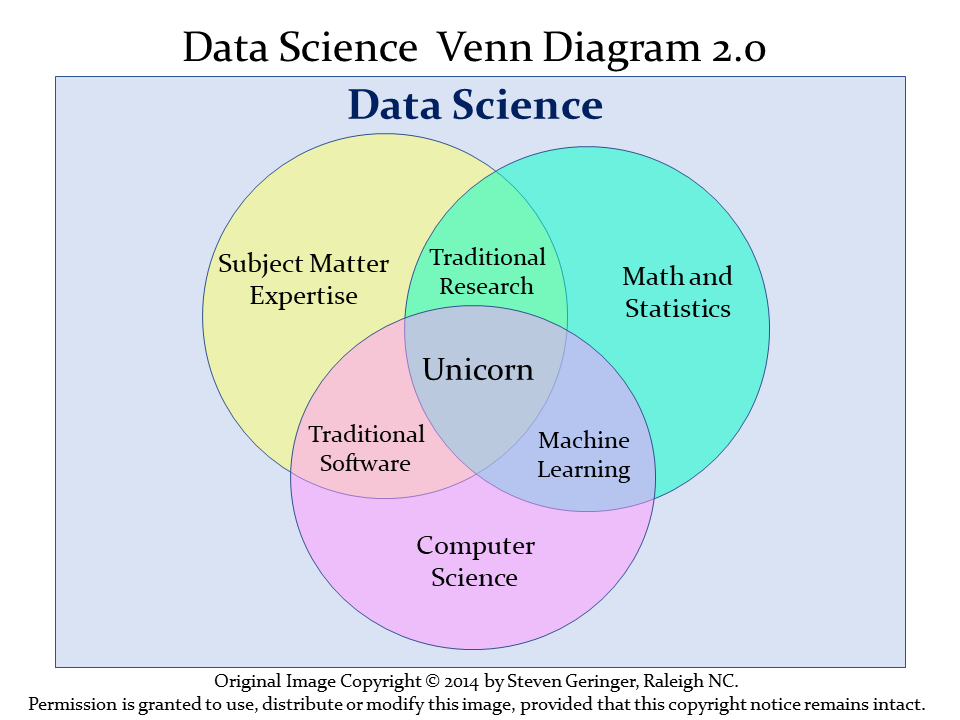
\includegraphics[width=0.8\linewidth]{figures/data-science-venn20} \caption{Data Science Venn Diagram from Steven Geringer}\label{fig:datasci-fig}
\end{figure}

\begin{itemize}
\tightlist
\item
  The field encompasses ideas from mathematics and statistics and from computer science, but with a heavy reliance on subject-matter knowledge. In our case, this includes clinical, health-related, medical or biological knowledge.
\item
  As \citet{Gelman-Nolan} suggest, the experience and intuition necessary for good statistical practice are hard to obtain, and teaching data science provides an excellent opportunity to reinforce statistical thinking skills across the full cycle of a data analysis project.
\item
  The principal form in which computer science (coding/programming) play a role in this course is to provide a form of communication. You'll need to learn how to express your ideas not just orally and in writing, but also through your code.
\end{itemize}

Data Science is a \textbf{team} activity. Everyone working in data science brings some part of the necessary skillset, but no one person can cover all three areas alone for excellent projects.

\begin{quote}
{[}The individual who is truly expert in all three key areas (mathematics/statistics, computer science and subject-matter knowledge) is{]} a mythical beast with magical powers who's rumored to exist but is never actually seen in the wild.

\url{http://www.kdnuggets.com/2016/10/battle-data-science-venn-diagrams.html}
\end{quote}

\hypertarget{data-science-project-cycle}{%
\section{Data Science Project Cycle}\label{data-science-project-cycle}}

A typical data science project can be modeled as follows, which comes from the introduction to the amazing book \textbf{R for Data Science}, by Garrett Grolemund and Hadley Wickham, which is a key text for this course \citep{R4DS}.

\begin{figure}
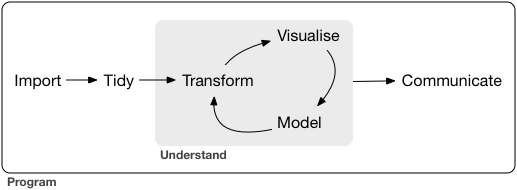
\includegraphics[width=0.95\linewidth]{figures/data-science-cycle} \caption{Source: R for Data Science: Introduction}\label{fig:cycle-fig}
\end{figure}

This diagram is sometimes referred to as the Krebs Cycle of Data Science. For more on the steps of a data science project, we encourage you to read the Introduction of \citet{R4DS}.

\hypertarget{data-science-and-the-431-course}{%
\section{Data Science and the 431 Course}\label{data-science-and-the-431-course}}

We'll discuss each of these elements in the 431 course, focusing at the start on understanding our data through transformation, modeling and (especially in the early stages) visualization. In 431, we learn how to get things done.

\begin{itemize}
\tightlist
\item
  We get people working with R and R Studio and R Markdown, even if they are completely new to coding. A gentle introduction is provided at \citet{ModernDive}
\item
  We learn how to use the \texttt{tidyverse} (\url{http://www.tidyverse.org/}), an array of tools in R (mostly developed by Hadley Wickham and his colleagues at R Studio) which share an underlying philosophy to make data science faster, easier, more reproducible and more fun. A critical text for understanding the tidyverse is \citet{R4DS}. Tidyverse tools facilitate:

  \begin{itemize}
  \tightlist
  \item
    \textbf{importing} data into R, which can be the source of intense pain for some things, but is really quite easy 95\% of the time with the right tool.
  \item
    \textbf{tidying} data, that is, storing it in a format that includes one row per observation and one column per variable. This is harder, and more important, than you might think.
  \item
    \textbf{transforming} data, perhaps by identifying specific subgroups of interest, creating new variables based on existing ones, or calculating summaries.
  \item
    \textbf{visualizing} data to generate actual knowledge and identify questions about the data - this is an area where R really shines, and we'll start with it in class.
  \item
    \textbf{modeling} data, taking the approach that modeling is complementary to visualization, and allows us to answer questions that visualization helps us identify.
  \item
    and last, but definitely not least, \textbf{communicating} results, models and visualizations to others, in a way that is reproducible and effective.
  \end{itemize}
\item
  Some programming/coding is an inevitable requirement to accomplish all of these aims. If you are leery of coding, you'll need to get past that, with the help of this course and our stellar teaching assistants. Getting started is always the most challenging part, but our experience is that most of the pain of developing these new skills evaporates by early October.
\end{itemize}

\hypertarget{what-the-course-is-and-isnt}{%
\section{What The Course Is and Isn't}\label{what-the-course-is-and-isnt}}

The 431 course is about \textbf{getting things done}. In developing this course, we adopt a modern approach that places data at the center of our work. Our goal is to teach you how to do truly reproducible research with modern tools. We want you to be able to collect and use data effectively to address questions of interest.

The curriculum includes more on several topics than you might expect from a standard graduate introduction to biostatistics.

\begin{itemize}
\tightlist
\item
  data gathering
\item
  data wrangling
\item
  exploratory data analysis and visualization
\item
  multivariate modeling
\item
  communication
\end{itemize}

It also nearly completely avoids formalism and is extremely applied - this is absolutely \textbf{not} a course in theoretical or mathematical statistics, and these Notes reflect that approach.

There's very little of the mathematical underpinnings here:

\[
f(x) = \frac{e^{-(x - \mu)^{2}/(2\sigma^{2})}}{\sigma{\sqrt{2 \pi }}} 
\]

Instead, these notes (and the course) focus on how we get R to do the things we want to do, and how we interpret the results of our work. Our next Chapter provides a first example.

\hypertarget{part-part-a.-exploring-data}{%
\part*{Part A. Exploring Data}\label{part-part-a.-exploring-data}}
\addcontentsline{toc}{part}{Part A. Exploring Data}

\hypertarget{looking-at-the-palmer-penguins}{%
\chapter{Looking at the Palmer Penguins}\label{looking-at-the-palmer-penguins}}

The data in the \texttt{palmerpenguins} package in R include size measurements, clutch observations, and blood isotope ratios for adult foraging Adélie, Chinstrap, and Gentoo penguins observed on islands in the Palmer Archipelago near Palmer Station, Antarctica. The data were collected and made available by Dr.~Kristen Gorman and the Palmer Station Long Term Ecological Research (LTER) Program.

For more on the \texttt{palmerpenguins} package, visit \url{https://allisonhorst.github.io/palmerpenguins/}.

\hypertarget{package-loading-then-dealing-with-missing-data}{%
\section{Package Loading, then Dealing with Missing Data}\label{package-loading-then-dealing-with-missing-data}}

To start, let's load up the necessary R packages to manage the data and summarize it in a small table, and a plot. We've actually done this previously, but we'll repeat the steps here, because it's worth seeing what R is doing.

In this case, we'll load up five packages.

\begin{Shaded}
\begin{Highlighting}[]
\KeywordTok{library}\NormalTok{(palmerpenguins)  }\CommentTok{# source for the data set}
\KeywordTok{library}\NormalTok{(janitor)         }\CommentTok{# some utilities for cleanup and simple tables}
\KeywordTok{library}\NormalTok{(magrittr)        }\CommentTok{# provides us with the pipe %>% for code management}
\KeywordTok{library}\NormalTok{(dplyr)           }\CommentTok{# part of the tidyverse: data management tools}
\KeywordTok{library}\NormalTok{(ggplot2)         }\CommentTok{# part of the tidyverse: tools for plotting data}
\end{Highlighting}
\end{Shaded}

It's worth remembering that everything after the \texttt{\#} on each line above is just a comment for the reader, and is ignored by R. We'll see later that the loading of a single package (called \texttt{tidyverse}) gives us both the \texttt{dplyr} and \texttt{ggplot2} packages, as well as several other useful things.

Next, let's take the \texttt{penguins} data from the \texttt{palmerpenguins} package, and identify those observations which have complete data (so, no missing values) in four variables of interest. We'll store that result in a new data frame (think of this as a data set) called \texttt{new\_penguins} and then take a look at that result using the following code.

\begin{Shaded}
\begin{Highlighting}[]
\NormalTok{new_penguins <-}\StringTok{ }\NormalTok{penguins }\OperatorTok
\StringTok{    }\KeywordTok{filter}\NormalTok{(}\KeywordTok{complete.cases}\NormalTok{(flipper_length_mm, body_mass_g, species, sex))}

\NormalTok{new_penguins}
\end{Highlighting}
\end{Shaded}

\begin{verbatim}
# A tibble: 333 x 8
   species island bill_length_mm bill_depth_mm flipper_length_~ body_mass_g
   <fct>   <fct>           <dbl>         <dbl>            <int>       <int>
 1 Adelie  Torge~           39.1          18.7              181        3750
 2 Adelie  Torge~           39.5          17.4              186        3800
 3 Adelie  Torge~           40.3          18                195        3250
 4 Adelie  Torge~           36.7          19.3              193        3450
 5 Adelie  Torge~           39.3          20.6              190        3650
 6 Adelie  Torge~           38.9          17.8              181        3625
 7 Adelie  Torge~           39.2          19.6              195        4675
 8 Adelie  Torge~           41.1          17.6              182        3200
 9 Adelie  Torge~           38.6          21.2              191        3800
10 Adelie  Torge~           34.6          21.1              198        4400
# ... with 323 more rows, and 2 more variables: sex <fct>, year <int>
\end{verbatim}

\hypertarget{counting-things-and-making-tables}{%
\section{Counting Things and Making Tables}\label{counting-things-and-making-tables}}

So, how many penguins are in our \texttt{new\_penguins} data? When we printed out the result, we got an answer, but (as with many things in R) there are many ways to get the same result.

\begin{Shaded}
\begin{Highlighting}[]
\KeywordTok{nrow}\NormalTok{(new_penguins)}
\end{Highlighting}
\end{Shaded}

\begin{verbatim}
[1] 333
\end{verbatim}

How do our \texttt{new\_penguins} data break down by sex and species?

\begin{Shaded}
\begin{Highlighting}[]
\NormalTok{new_penguins }\OperatorTok\StringTok{ }
\StringTok{    }\KeywordTok{tabyl}\NormalTok{(sex, species) }\CommentTok{# tabyl comes from the janitor package}
\end{Highlighting}
\end{Shaded}

\begin{verbatim}
    sex Adelie Chinstrap Gentoo
 female     73        34     58
   male     73        34     61
\end{verbatim}

Note the strange spelling of \texttt{tabyl} here. The output is reasonably clear, but could we make that table a little prettier, and while we're at it, can we add the row and column totals to it?

\begin{Shaded}
\begin{Highlighting}[]
\NormalTok{new_penguins }\OperatorTok\StringTok{ }
\StringTok{    }\KeywordTok{tabyl}\NormalTok{(sex, species) }\OperatorTok
\StringTok{    }\KeywordTok{adorn_totals}\NormalTok{(}\DataTypeTok{where =} \KeywordTok{c}\NormalTok{(}\StringTok{"row"}\NormalTok{, }\StringTok{"col"}\NormalTok{)) }\OperatorTok\StringTok{ }\CommentTok{# add row, column totals}
\StringTok{    }\NormalTok{kable  }\CommentTok{# one convenient way to make the table prettier}
\end{Highlighting}
\end{Shaded}

\begin{tabular}{l|r|r|r|r}
\hline
sex & Adelie & Chinstrap & Gentoo & Total\\
\hline
female & 73 & 34 & 58 & 165\\
\hline
male & 73 & 34 & 61 & 168\\
\hline
Total & 146 & 68 & 119 & 333\\
\hline
\end{tabular}

\hypertarget{visualizing-the-data-in-a-graph-or-a-few}{%
\section{Visualizing the Data in a Graph (or a few\ldots)}\label{visualizing-the-data-in-a-graph-or-a-few}}

Now, let's look at the other two variables of interest. Let's create a graph showing the association of body mass with flipper length across the complete set of 333 penguins.

\begin{Shaded}
\begin{Highlighting}[]
\KeywordTok{ggplot}\NormalTok{(new_penguins, }\KeywordTok{aes}\NormalTok{(}\DataTypeTok{x =}\NormalTok{ body_mass_g, }\DataTypeTok{y =}\NormalTok{ flipper_length_mm)) }\OperatorTok{+}
\StringTok{    }\KeywordTok{geom_point}\NormalTok{() }
\end{Highlighting}
\end{Shaded}

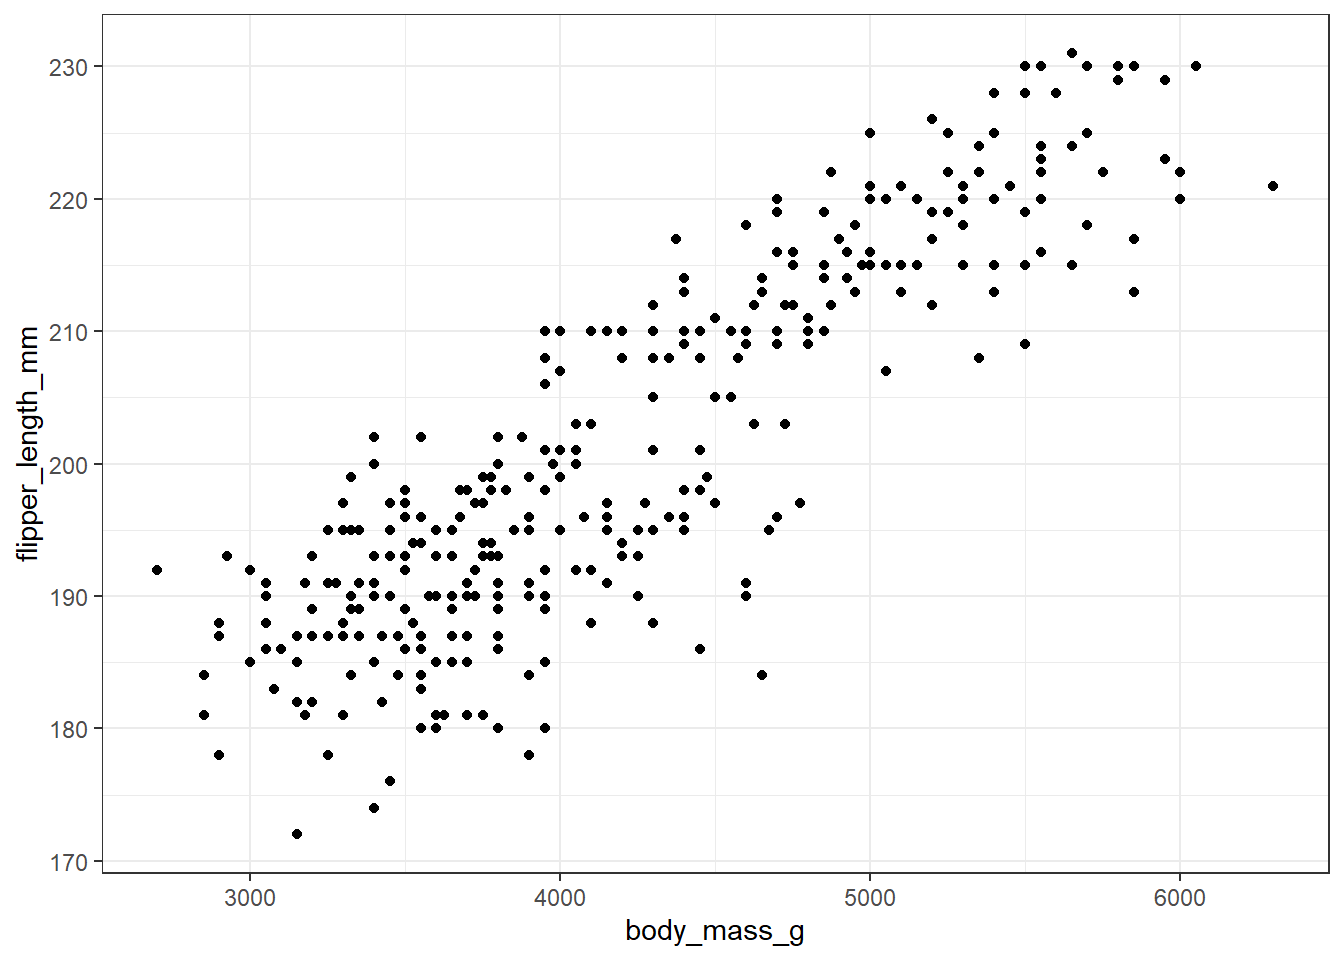
\includegraphics{431-notes_files/figure-latex/unnamed-chunk-6-1.pdf}

Some of you may want to include a straight-line model (fit by a classical linear regression) to this plot. One way to do that in R involves the addition of a single line of code, like this:

\begin{Shaded}
\begin{Highlighting}[]
\KeywordTok{ggplot}\NormalTok{(new_penguins, }\KeywordTok{aes}\NormalTok{(}\DataTypeTok{x =}\NormalTok{ body_mass_g, }\DataTypeTok{y =}\NormalTok{ flipper_length_mm)) }\OperatorTok{+}
\StringTok{    }\KeywordTok{geom_point}\NormalTok{() }\OperatorTok{+}
\StringTok{    }\KeywordTok{geom_smooth}\NormalTok{(}\DataTypeTok{method =} \StringTok{"lm"}\NormalTok{, }\DataTypeTok{col =} \StringTok{"red"}\NormalTok{, }\DataTypeTok{se =} \OtherTok{FALSE}\NormalTok{)}
\end{Highlighting}
\end{Shaded}

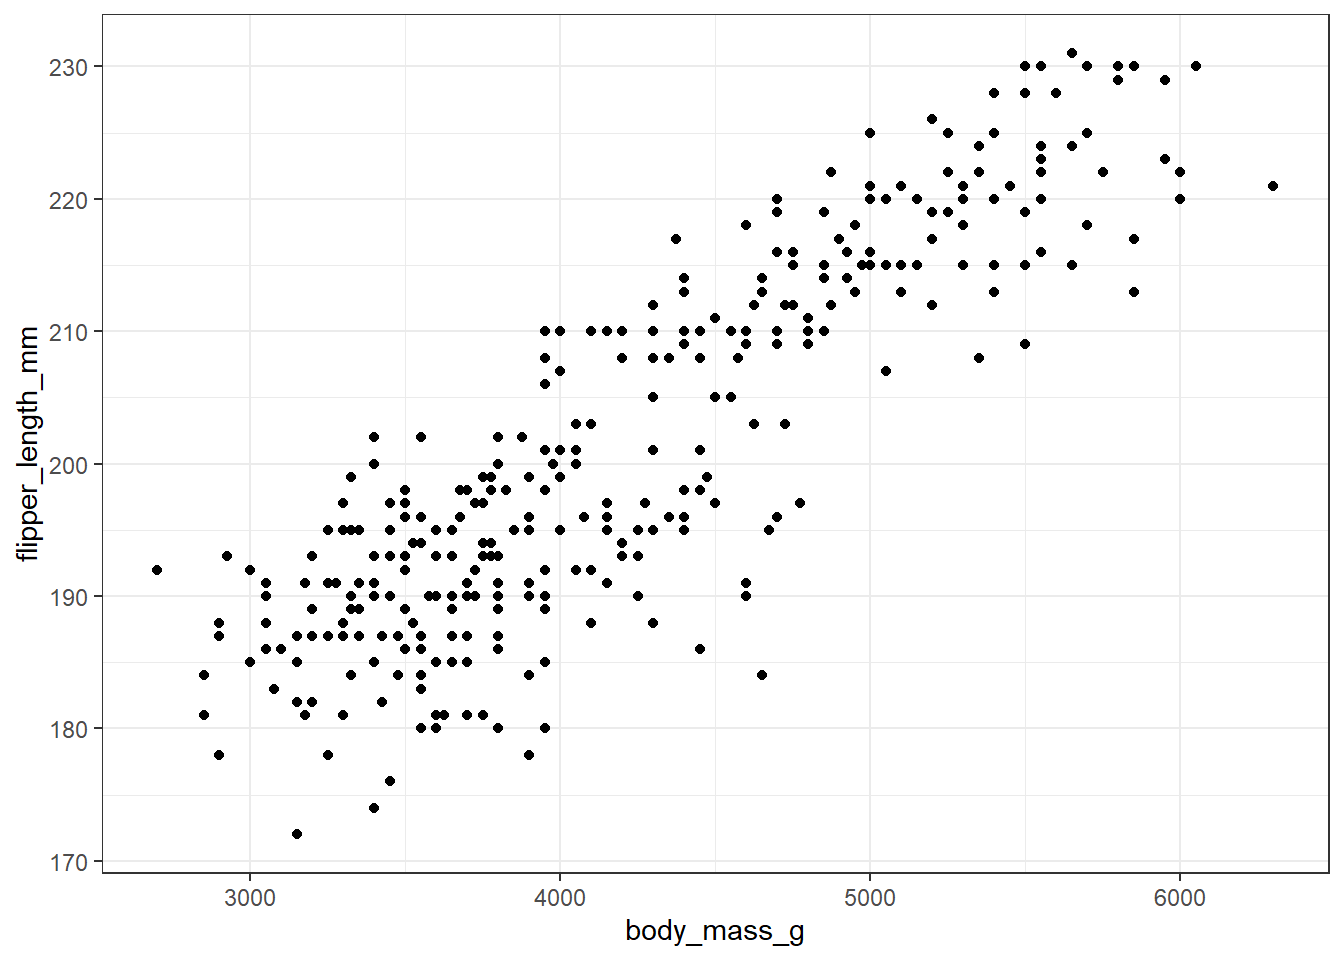
\includegraphics{431-notes_files/figure-latex/unnamed-chunk-7-1.pdf}

Whenever we build a graph for ourselves, these default choices may be sufficient. But I'd like to see a prettier version if I was going to show it to someone else. So, I might use a different color for each species, and I might neaten up the theme (to get rid of the default grey background) and add a title, like this.

\begin{Shaded}
\begin{Highlighting}[]
\KeywordTok{ggplot}\NormalTok{(new_penguins, }\KeywordTok{aes}\NormalTok{(}\DataTypeTok{x =}\NormalTok{ body_mass_g, }\DataTypeTok{y =}\NormalTok{ flipper_length_mm, }\DataTypeTok{col =}\NormalTok{ species)) }\OperatorTok{+}
\StringTok{    }\KeywordTok{geom_point}\NormalTok{() }\OperatorTok{+}\StringTok{ }
\StringTok{    }\KeywordTok{theme_bw}\NormalTok{() }\OperatorTok{+}\StringTok{ }
\StringTok{    }\KeywordTok{labs}\NormalTok{(}\DataTypeTok{title =} \StringTok{"Flipper Length and Body Mass for 333 of the Palmer Penguins"}\NormalTok{)}
\end{Highlighting}
\end{Shaded}

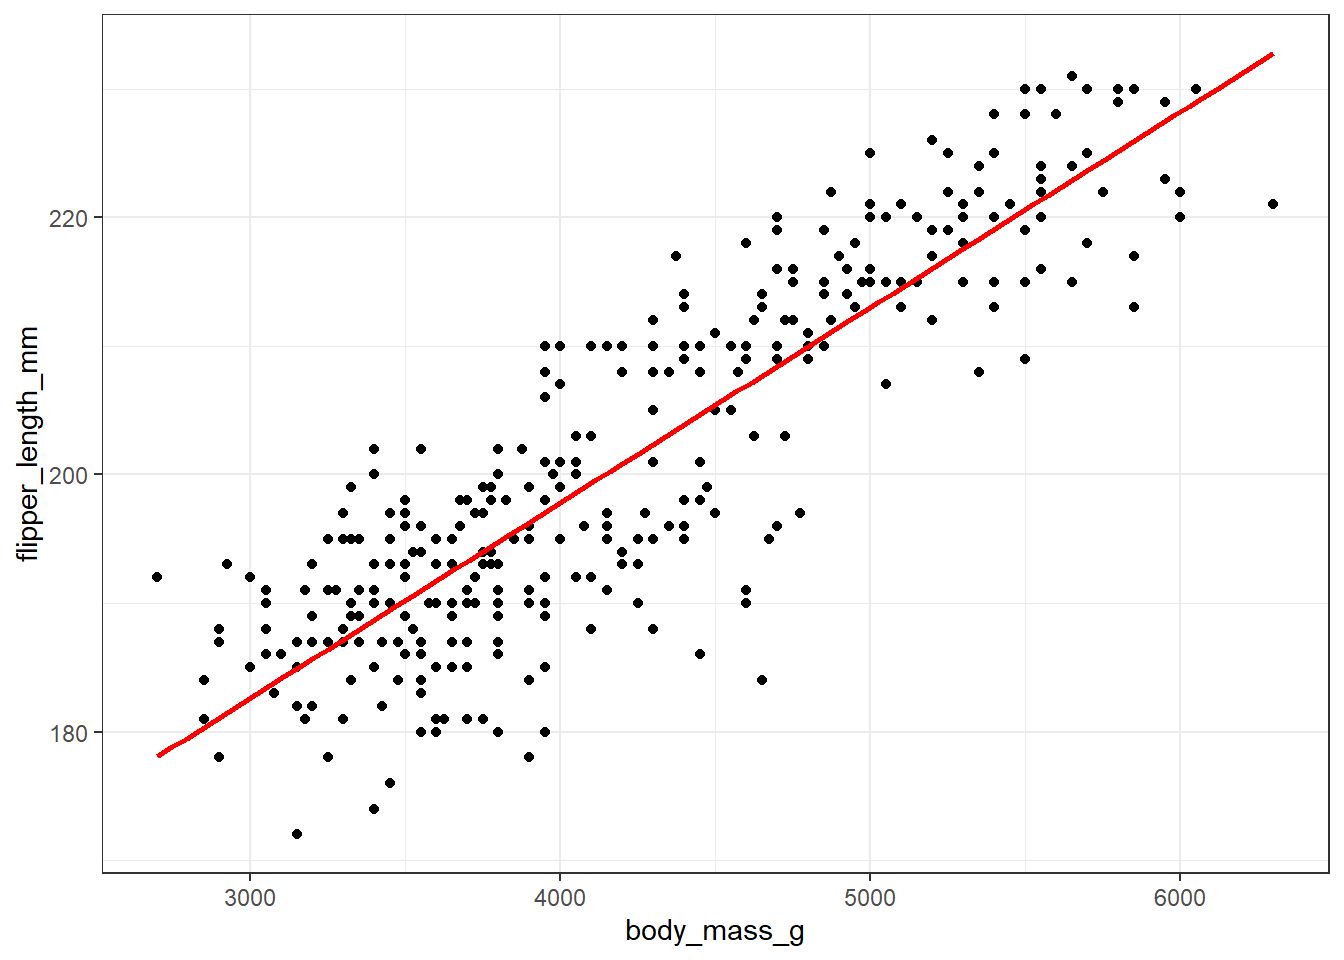
\includegraphics{431-notes_files/figure-latex/unnamed-chunk-8-1.pdf}

\hypertarget{six-ways-to-improve-this-graph}{%
\section{Six Ways To ``Improve'' This Graph}\label{six-ways-to-improve-this-graph}}

Now, let's build a new graph. Here, I want to:

\begin{enumerate}
\def\labelenumi{\arabic{enumi}.}
\tightlist
\item
  plot the relationship between body mass and flipper length in light of both Sex and Species
\item
  increase the size of the points and add a little transparency so we can see if points overlap,
\item
  add some smooth curves to summarize the relationships between the two quantities (body mass and flipper length) within each combination of species and sex,
\item
  split the graph into two ``facets'' (one for each sex),
\item
  improve the axis labels,
\item
  improve the titles by adding a subtitle, and also adding in some code to count the penguins (rather than hard-coding in the total number.)
\end{enumerate}

\begin{Shaded}
\begin{Highlighting}[]
\KeywordTok{ggplot}\NormalTok{(new_penguins, }\KeywordTok{aes}\NormalTok{(}\DataTypeTok{x =}\NormalTok{ body_mass_g, }\DataTypeTok{y =}\NormalTok{ flipper_length_mm, }
                         \DataTypeTok{col =}\NormalTok{ species)) }\OperatorTok{+}
\StringTok{    }\KeywordTok{geom_point}\NormalTok{(}\DataTypeTok{size =} \DecValTok{2}\NormalTok{, }\DataTypeTok{alpha =} \FloatTok{0.5}\NormalTok{) }\OperatorTok{+}\StringTok{ }
\StringTok{    }\KeywordTok{geom_smooth}\NormalTok{(}\DataTypeTok{method =} \StringTok{"loess"}\NormalTok{, }\DataTypeTok{se =} \OtherTok{FALSE}\NormalTok{, }\DataTypeTok{size =} \FloatTok{1.5}\NormalTok{) }\OperatorTok{+}
\StringTok{    }\KeywordTok{facet_grid}\NormalTok{(}\OperatorTok{~}\StringTok{ }\NormalTok{sex) }\OperatorTok{+}
\StringTok{    }\KeywordTok{theme_bw}\NormalTok{() }\OperatorTok{+}\StringTok{ }
\StringTok{    }\KeywordTok{labs}\NormalTok{(}\DataTypeTok{title =} \StringTok{"Flipper Length and Body Mass, by Sex & Species"}\NormalTok{,}
         \DataTypeTok{subtitle =} \KeywordTok{paste0}\NormalTok{(}\KeywordTok{nrow}\NormalTok{(new_penguins), }\StringTok{" of the Palmer Penguins"}\NormalTok{),}
         \DataTypeTok{x =} \StringTok{"Body Mass (g)"}\NormalTok{, }
         \DataTypeTok{y =} \StringTok{"Flipper Length (mm)"}\NormalTok{)}
\end{Highlighting}
\end{Shaded}

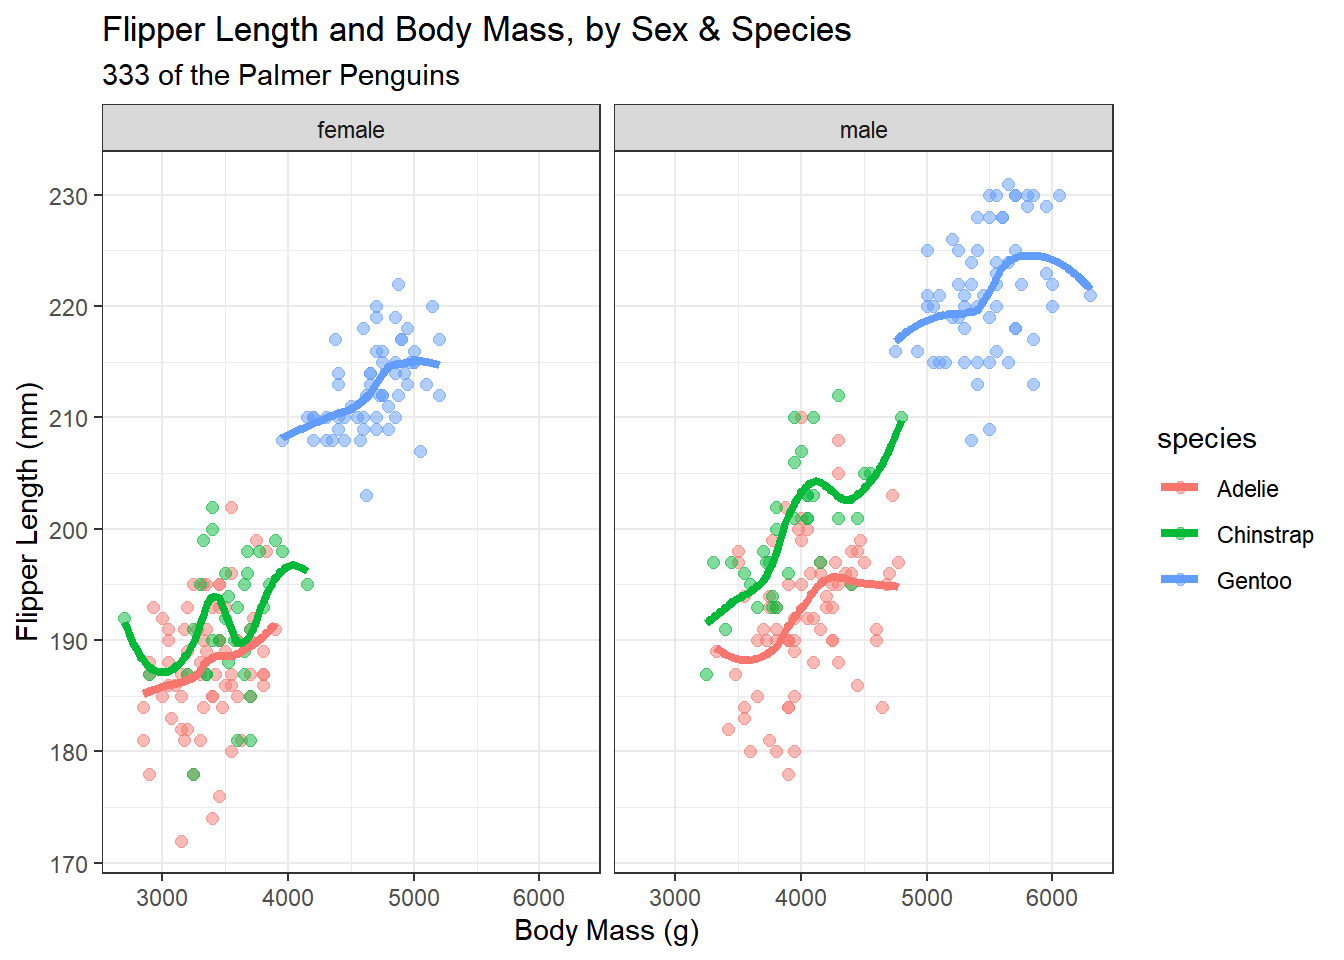
\includegraphics{431-notes_files/figure-latex/unnamed-chunk-9-1.pdf}

\hypertarget{a-little-reflection}{%
\section{A Little Reflection}\label{a-little-reflection}}

What can we learn from these plots and their construction? In particular,

\begin{itemize}
\tightlist
\item
  What do these plots suggest about the center of the distribution of each quantity (body mass and flipper length) overall, and within each combination of Sex and Species?
\item
  What does the final plot suggest about the spread of the distribution of each of those quantities in each combination of Sex and Species?
\item
  What do the plots suggest about the association of body mass and flipper length across the complete set of penguins?
\item
  How does the shape and nature of this body mass - flipper length relationship change based on Sex and Species?
\item
  Do you think it would be helpful to plot a straight-line relationship (rather than a smooth curve) within each combination of Sex and Species in the final plot? Why or why not? (Also, what would we have to do to the code to accomplish this?)
\item
  How was the R code for the plot revised to accomplish each of the six ``wants'' specified above?
\end{itemize}

\hypertarget{dataviz}{%
\chapter{NHANES: Initial Exploring}\label{dataviz}}

We'll start by visualizing some data from the US National Health and Nutrition Examination Survey, or NHANES. We'll display R code as we go, but we'll return to all of the key coding ideas involved later in the Notes.

\hypertarget{the-nhanes-data-collecting-a-sample}{%
\section{The NHANES data: Collecting a Sample}\label{the-nhanes-data-collecting-a-sample}}

To begin, we'll gather a random sample of 1,000 subjects participating in NHANES, and then identify several variables of interest about those subjects\footnote{For more on the NHANES data available in the NHANES package, type ?NHANES in the Console in R Studio.}. Some of the motivation for this example came from a Figure in \citet{BaumerKaplanHorton}.

\begin{Shaded}
\begin{Highlighting}[]
\CommentTok{# library(NHANES) # already loaded NHANES package/library of functions, data}

\KeywordTok{set.seed}\NormalTok{(}\DecValTok{431001}\NormalTok{) }
\CommentTok{# use set.seed to ensure that we all get the same random sample }
\CommentTok{# of 1,000 NHANES subjects in our nh_data collection}

\NormalTok{nh_dat1 <-}\StringTok{ }\KeywordTok{sample_n}\NormalTok{(NHANES, }\DataTypeTok{size =} \DecValTok{1000}\NormalTok{) }\OperatorTok
\StringTok{    }\KeywordTok{select}\NormalTok{(ID, Gender, Age, Height) }

\NormalTok{nh_dat1}
\end{Highlighting}
\end{Shaded}

\begin{verbatim}
# A tibble: 1,000 x 4
      ID Gender   Age Height
   <int> <fct>  <int>  <dbl>
 1 69638 female     5   106.
 2 70782 male      64   176.
 3 52408 female    54   162.
 4 59031 female    15   155.
 5 64530 male      53   185.
 6 71040 male      63   169.
 7 55186 female    30   168.
 8 60211 male       5   103.
 9 55730 male      66   161.
10 68229 female    36   170.
# ... with 990 more rows
\end{verbatim}

We have 1000 rows (observations) and 4 columns (variables) that describe the subjects listed in the rows.

\hypertarget{age-and-height}{%
\section{Age and Height}\label{age-and-height}}

Suppose we want to visualize the relationship of Height and Age in our 1,000 NHANES observations. The best choice is likely to be a scatterplot.

\begin{Shaded}
\begin{Highlighting}[]
\KeywordTok{ggplot}\NormalTok{(}\DataTypeTok{data =}\NormalTok{ nh_dat1, }\KeywordTok{aes}\NormalTok{(}\DataTypeTok{x =}\NormalTok{ Age, }\DataTypeTok{y =}\NormalTok{ Height)) }\OperatorTok{+}
\StringTok{    }\KeywordTok{geom_point}\NormalTok{()}
\end{Highlighting}
\end{Shaded}

\begin{verbatim}
Warning: Removed 37 rows containing missing values (geom_point).
\end{verbatim}

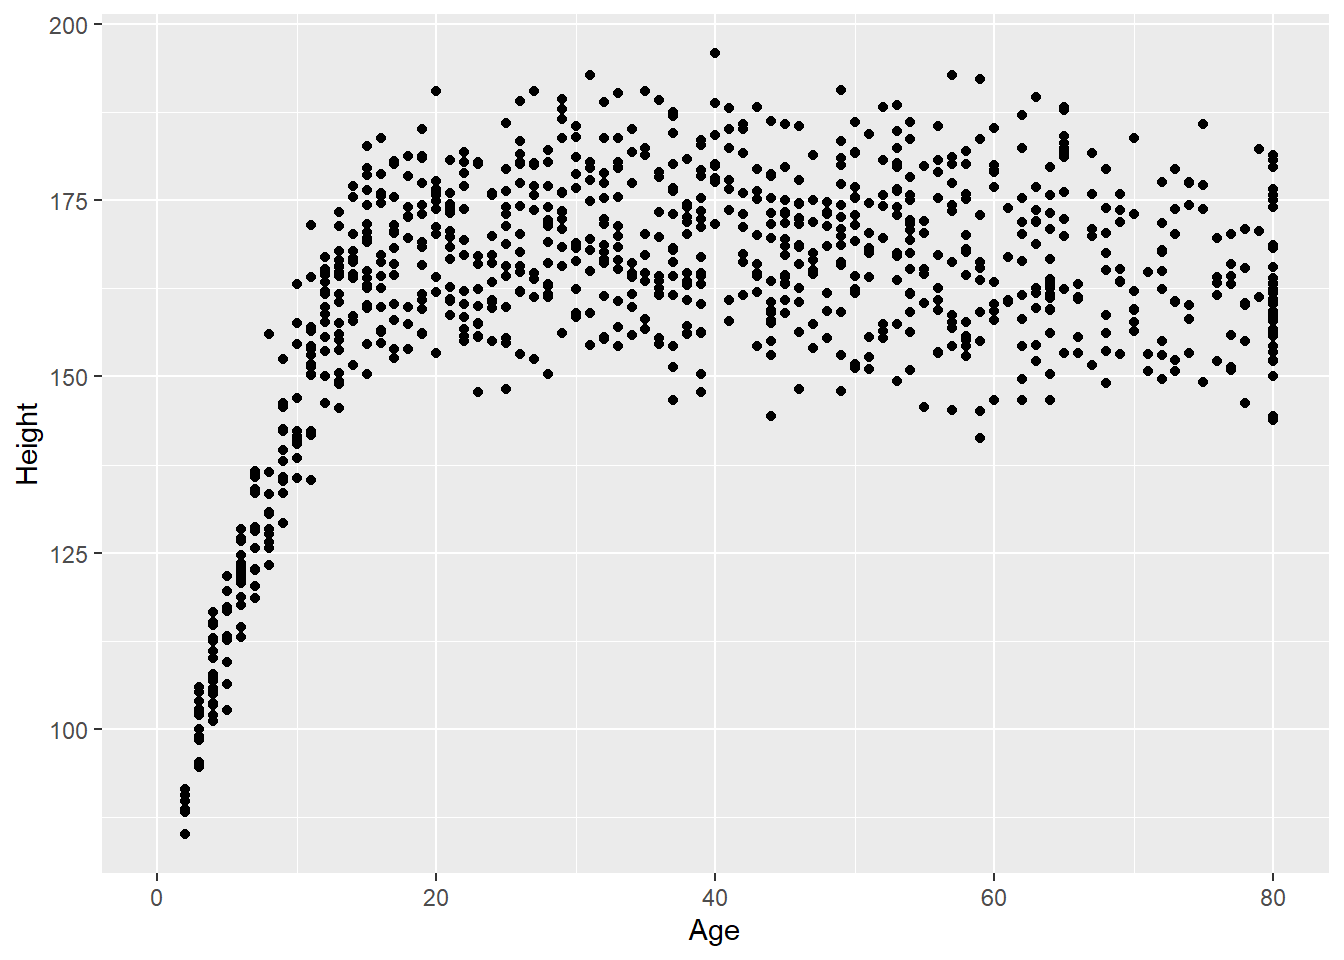
\includegraphics{431-notes_files/figure-latex/nh_dat1_heightbyage1-fig-1.pdf}

We note several interesting results here.

\begin{enumerate}
\def\labelenumi{\arabic{enumi}.}
\tightlist
\item
  As a warning, R tells us that it has ``Removed 37 rows containing missing values (geom\_point).'' Only 963 subjects plotted here, because the remaining 37 people have missing (NA) values for either Height, Age or both.
\item
  Unsurprisingly, the measured Heights of subjects grow from Age 0 to Age 20 or so, and we see that a typical Height increases rapidly across these Ages. The middle of the distribution at later Ages is pretty consistent at at a Height somewhere between 150 and 175. The units aren't specified, but we expect they must be centimeters. The Ages are clearly reported in Years.
\item
  No Age is reported over 80, and it appears that there is a large cluster of Ages at 80. This may be due to a requirement that Ages 80 and above be reported at 80 so as to help mask the identity of those individuals.\footnote{If you visit the NHANES help file with ?NHANES, you will see that subjects 80 years or older were indeed recorded as 80.}
\end{enumerate}

As in this case, we're going to build most of our visualizations using tools from the \texttt{ggplot2} package, which is part of the \texttt{tidyverse} series of packages. You'll see similar coding structures throughout this Chapter, most of which are covered as well in Chapter 3 of \citet{R4DS}.

\hypertarget{subset-of-subjects-with-known-age-and-height}{%
\section{Subset of Subjects with Known Age and Height}\label{subset-of-subjects-with-known-age-and-height}}

Before we move on, let's manipulate the data set a bit, to focus on only those subjects who have complete data on both Age and Height. This will help us avoid that warning message.

\begin{Shaded}
\begin{Highlighting}[]
\NormalTok{nh_dat2 <-}\StringTok{ }\NormalTok{nh_dat1 }\OperatorTok
\StringTok{    }\KeywordTok{filter}\NormalTok{(}\KeywordTok{complete.cases}\NormalTok{(Age, Height)) }

\KeywordTok{summary}\NormalTok{(nh_dat2)}
\end{Highlighting}
\end{Shaded}

\begin{verbatim}
       ID           Gender         Age            Height     
 Min.   :51624   female:484   Min.   : 2.00   Min.   : 85.0  
 1st Qu.:57034   male  :479   1st Qu.:19.00   1st Qu.:156.2  
 Median :62056                Median :37.00   Median :165.0  
 Mean   :61967                Mean   :38.29   Mean   :162.3  
 3rd Qu.:67269                3rd Qu.:56.00   3rd Qu.:174.5  
 Max.   :71875                Max.   :80.00   Max.   :195.9  
\end{verbatim}

Note that the units and explanations for these variables are contained in the NHANES help file, available via typing \texttt{?NHANES} in the Console of R Studio, or by typing \texttt{NHANES} into the Search bar in R Studio's Help window.

\hypertarget{the-distinction-between-gender-and-sex}{%
\subsection{\texorpdfstring{The Distinction between \texttt{Gender} and \texttt{Sex}}{The Distinction between Gender and Sex}}\label{the-distinction-between-gender-and-sex}}

The \texttt{Gender} variable here is a mistake. These data refer to the biological status of these subjects, which is their \texttt{Sex}, and not the social construct of \texttt{Gender} which can be quite different. In our effort to avoid further confusion, we'll rename the variable \texttt{Gender} to instead more accurately describe what is actually measured here.

To do this, we can use this approach\ldots{}

\begin{Shaded}
\begin{Highlighting}[]
\NormalTok{nh_dat2 <-}\StringTok{ }\NormalTok{nh_dat1 }\OperatorTok
\StringTok{    }\KeywordTok{rename}\NormalTok{(}\DataTypeTok{Sex =}\NormalTok{ Gender) }\OperatorTok
\StringTok{    }\KeywordTok{filter}\NormalTok{(}\KeywordTok{complete.cases}\NormalTok{(Age, Height)) }

\KeywordTok{summary}\NormalTok{(nh_dat2)}
\end{Highlighting}
\end{Shaded}

\begin{verbatim}
       ID            Sex           Age            Height     
 Min.   :51624   female:484   Min.   : 2.00   Min.   : 85.0  
 1st Qu.:57034   male  :479   1st Qu.:19.00   1st Qu.:156.2  
 Median :62056                Median :37.00   Median :165.0  
 Mean   :61967                Mean   :38.29   Mean   :162.3  
 3rd Qu.:67269                3rd Qu.:56.00   3rd Qu.:174.5  
 Max.   :71875                Max.   :80.00   Max.   :195.9  
\end{verbatim}

That's better. How many observations do we have now? We could use \texttt{dim} to find out the number of rows and columns in this new data set.

\begin{Shaded}
\begin{Highlighting}[]
\KeywordTok{dim}\NormalTok{(nh_dat2)}
\end{Highlighting}
\end{Shaded}

\begin{verbatim}
[1] 963   4
\end{verbatim}

Or, we could simply list the data set and read off the result.

\begin{Shaded}
\begin{Highlighting}[]
\NormalTok{nh_dat2}
\end{Highlighting}
\end{Shaded}

\begin{verbatim}
# A tibble: 963 x 4
      ID Sex      Age Height
   <int> <fct>  <int>  <dbl>
 1 69638 female     5   106.
 2 70782 male      64   176.
 3 52408 female    54   162.
 4 59031 female    15   155.
 5 64530 male      53   185.
 6 71040 male      63   169.
 7 55186 female    30   168.
 8 60211 male       5   103.
 9 55730 male      66   161.
10 68229 female    36   170.
# ... with 953 more rows
\end{verbatim}

\hypertarget{age-height-and-sex}{%
\section{Age-Height and Sex?}\label{age-height-and-sex}}

Let's add Sex to the plot using color, and also adjust the y axis label to incorporate the units of measurement.

\begin{Shaded}
\begin{Highlighting}[]
\KeywordTok{ggplot}\NormalTok{(}\DataTypeTok{data =}\NormalTok{ nh_dat2, }\KeywordTok{aes}\NormalTok{(}\DataTypeTok{x =}\NormalTok{ Age, }\DataTypeTok{y =}\NormalTok{ Height, }\DataTypeTok{color =}\NormalTok{ Sex)) }\OperatorTok{+}
\StringTok{    }\KeywordTok{geom_point}\NormalTok{() }\OperatorTok{+}
\StringTok{    }\KeywordTok{labs}\NormalTok{(}\DataTypeTok{title =} \StringTok{"Height-Age Relationship in NHANES sample"}\NormalTok{, }
         \DataTypeTok{y =} \StringTok{"Height in cm."}\NormalTok{)}
\end{Highlighting}
\end{Shaded}

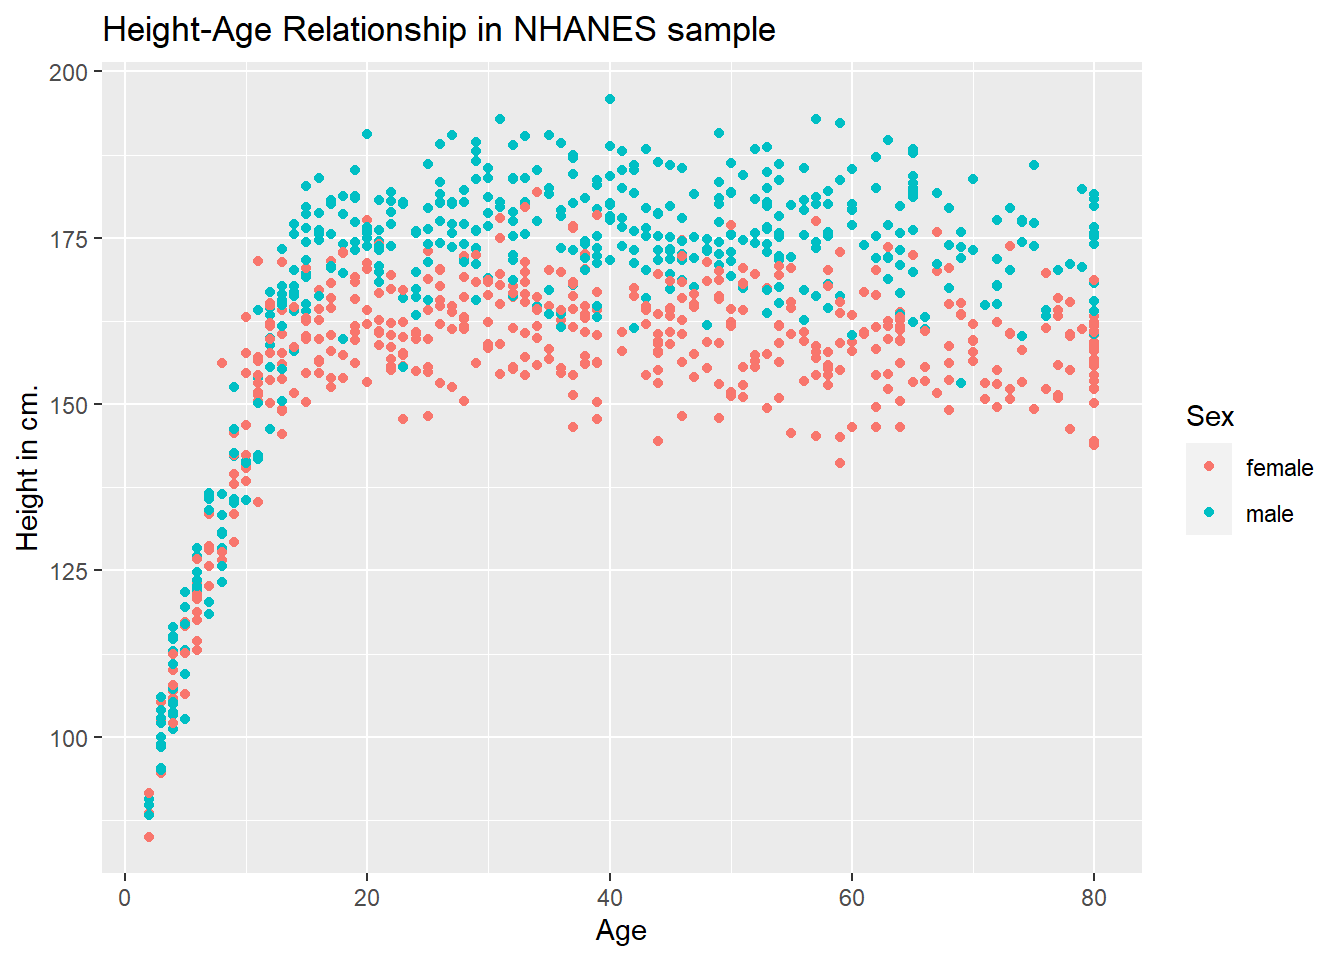
\includegraphics{431-notes_files/figure-latex/nh_dat2_heightbyageandsex1-fig-1.pdf}

\hypertarget{can-we-show-the-female-and-male-relationships-in-separate-panels}{%
\subsection{Can we show the Female and Male relationships in separate panels?}\label{can-we-show-the-female-and-male-relationships-in-separate-panels}}

Sure.

\begin{Shaded}
\begin{Highlighting}[]
\KeywordTok{ggplot}\NormalTok{(}\DataTypeTok{data =}\NormalTok{ nh_dat2, }\KeywordTok{aes}\NormalTok{(}\DataTypeTok{x =}\NormalTok{ Age, }\DataTypeTok{y =}\NormalTok{ Height, }\DataTypeTok{color =}\NormalTok{ Sex)) }\OperatorTok{+}
\StringTok{    }\KeywordTok{geom_point}\NormalTok{() }\OperatorTok{+}\StringTok{ }
\StringTok{    }\KeywordTok{labs}\NormalTok{(}\DataTypeTok{title =} \StringTok{"Height-Age Relationship in NHANES sample"}\NormalTok{, }
         \DataTypeTok{y =} \StringTok{"Height in cm."}\NormalTok{) }\OperatorTok{+}
\StringTok{    }\KeywordTok{facet_wrap}\NormalTok{(}\OperatorTok{~}\StringTok{ }\NormalTok{Sex)}
\end{Highlighting}
\end{Shaded}

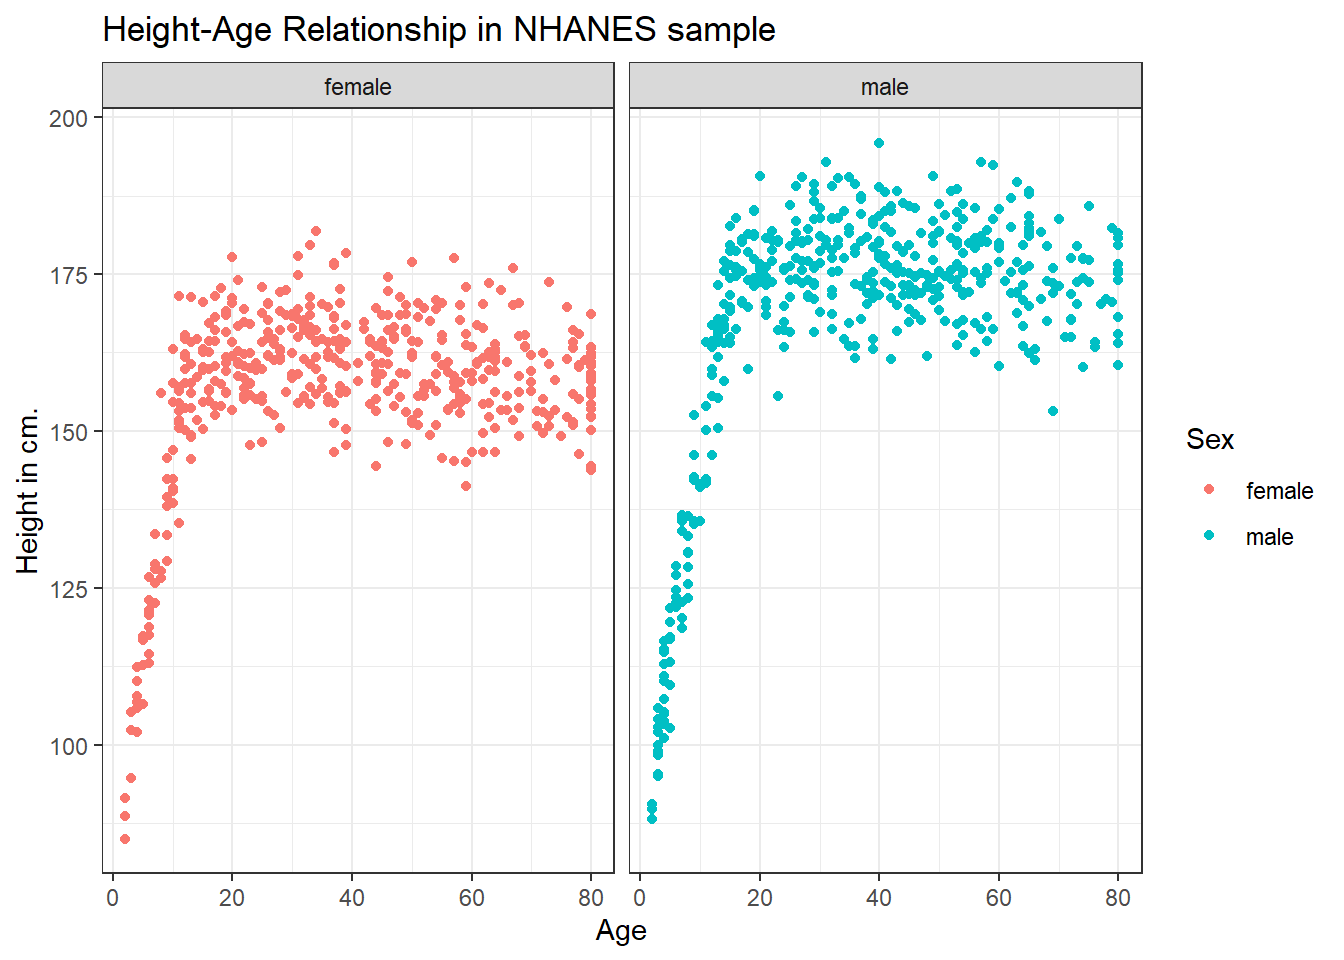
\includegraphics{431-notes_files/figure-latex/nh_dat2_heightbyageandsex2-fig-1.pdf}

\hypertarget{can-we-add-a-smooth-curve-to-show-the-relationship-in-each-plot}{%
\subsection{Can we add a smooth curve to show the relationship in each plot?}\label{can-we-add-a-smooth-curve-to-show-the-relationship-in-each-plot}}

Yep, and let's change the theme of the graph to remove the gray background, too.

\begin{Shaded}
\begin{Highlighting}[]
\KeywordTok{ggplot}\NormalTok{(}\DataTypeTok{data =}\NormalTok{ nh_dat2, }\KeywordTok{aes}\NormalTok{(}\DataTypeTok{x =}\NormalTok{ Age, }\DataTypeTok{y =}\NormalTok{ Height, }\DataTypeTok{color =}\NormalTok{ Sex)) }\OperatorTok{+}
\StringTok{    }\KeywordTok{geom_point}\NormalTok{() }\OperatorTok{+}\StringTok{ }
\StringTok{    }\KeywordTok{geom_smooth}\NormalTok{(}\DataTypeTok{method =} \StringTok{"loess"}\NormalTok{) }\OperatorTok{+}
\StringTok{    }\KeywordTok{labs}\NormalTok{(}\DataTypeTok{title =} \StringTok{"Height-Age Relationship in NHANES sample"}\NormalTok{, }
         \DataTypeTok{y =} \StringTok{"Height in cm."}\NormalTok{) }\OperatorTok{+}
\StringTok{    }\KeywordTok{theme_bw}\NormalTok{() }\OperatorTok{+}
\StringTok{    }\KeywordTok{facet_wrap}\NormalTok{(}\OperatorTok{~}\StringTok{ }\NormalTok{Sex)}
\end{Highlighting}
\end{Shaded}

\begin{verbatim}
`geom_smooth()` using formula 'y ~ x'
\end{verbatim}

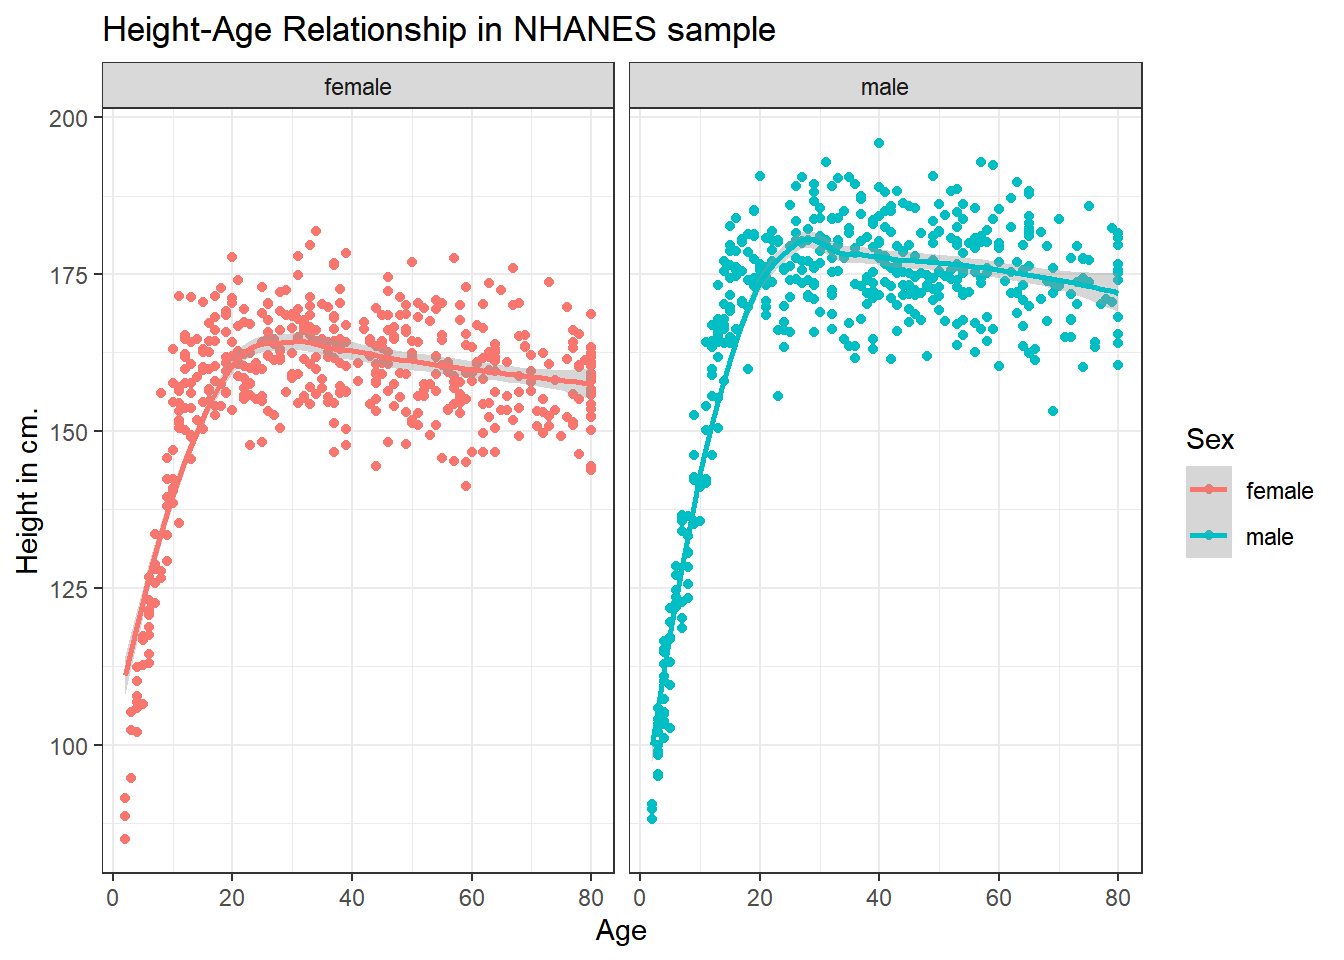
\includegraphics{431-notes_files/figure-latex/nh_dat2_heightbyageandsex3-fig-1.pdf}

\hypertarget{what-if-we-want-to-assume-straight-line-relationships}{%
\subsection{What if we want to assume straight line relationships?}\label{what-if-we-want-to-assume-straight-line-relationships}}

We could look at a linear model in the plot. Does this make sense here?

\begin{Shaded}
\begin{Highlighting}[]
\KeywordTok{ggplot}\NormalTok{(}\DataTypeTok{data =}\NormalTok{ nh_dat2, }\KeywordTok{aes}\NormalTok{(}\DataTypeTok{x =}\NormalTok{ Age, }\DataTypeTok{y =}\NormalTok{ Height, }\DataTypeTok{color =}\NormalTok{ Sex)) }\OperatorTok{+}
\StringTok{    }\KeywordTok{geom_point}\NormalTok{() }\OperatorTok{+}\StringTok{ }
\StringTok{    }\KeywordTok{geom_smooth}\NormalTok{(}\DataTypeTok{method =} \StringTok{"lm"}\NormalTok{) }\OperatorTok{+}
\StringTok{    }\KeywordTok{labs}\NormalTok{(}\DataTypeTok{title =} \StringTok{"Height-Age Relationship in NHANES sample"}\NormalTok{, }
         \DataTypeTok{y =} \StringTok{"Height in cm."}\NormalTok{) }\OperatorTok{+}
\StringTok{    }\KeywordTok{theme_bw}\NormalTok{() }\OperatorTok{+}
\StringTok{    }\KeywordTok{facet_wrap}\NormalTok{(}\OperatorTok{~}\StringTok{ }\NormalTok{Sex)}
\end{Highlighting}
\end{Shaded}

\begin{verbatim}
`geom_smooth()` using formula 'y ~ x'
\end{verbatim}

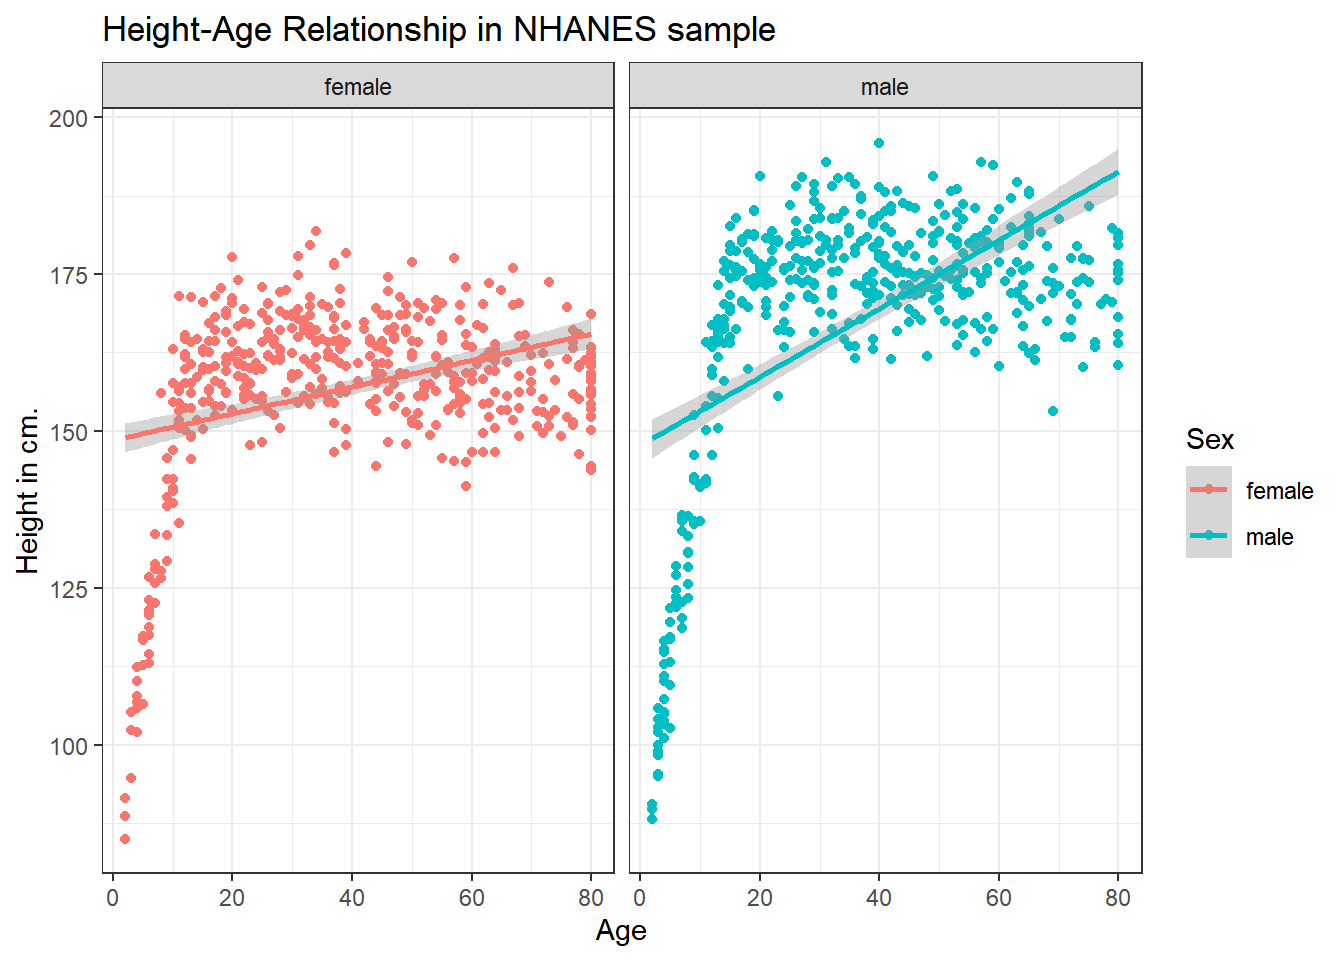
\includegraphics{431-notes_files/figure-latex/nh_dat2_heightbyageandsex4-fig-1.pdf}

\hypertarget{creating-a-new-subset-ages-21-79}{%
\section{Creating A New Subset: Ages 21-79}\label{creating-a-new-subset-ages-21-79}}

Suppose we wanted to look only at those observations (subjects) whose Age is at least 21 and at most 79. Suppose also that we want to look at some of the additional variables available in NHANES. To start, we'll do the following:

\begin{enumerate}
\def\labelenumi{\arabic{enumi}.}
\tightlist
\item
  Set the same seed for random sampling that we used earlier, so that we start with the original sample of 1000 people we built earlier. Draw that same sample of 1,000 people.
\item
  Filter the sample to only those people whose age is more than 20 and less than 80 years.
\item
  Select the variables we will use in the rest of this chapter:

  \begin{itemize}
  \tightlist
  \item
    \texttt{Age} as we've seen before, in years.
  \item
    \texttt{Height} as we've seen before, in centimeters.
  \item
    \texttt{Gender} which we'll rename as \texttt{Sex} again.
  \item
    \texttt{Pulse} = 60 second pulse rate (in beats per minute).
  \item
    \texttt{BPSysAve} = Systolic Blood Pressure, in mm Hg (and we'll rename this \texttt{SBP}).
  \item
    \texttt{SleepTrouble} = Yes means the subject has told a health professional that they had trouble sleeping.
  \item
    \texttt{PhysActive} = Yes means the subject does moderate or vigorous-intensity sports, fitness or recreational activity.
  \item
    \texttt{MaritalStatus} = one of Married, Widowed, Divorced, Separated, NeverMarried or LivePartner (living with partner.)
  \item
    \texttt{HealthGen} = self-reported rating of general health, one of Excellent, Vgood (Very Good), Good, Fair or Poor.
  \end{itemize}
\item
  Rename \texttt{Gender} as \texttt{Sex}, to more accurately describe what is being measured.
\item
  Omit subjects with any missingness on \emph{any} of the variables we've selected.
\end{enumerate}

Can you see how the code below accomplishes these tasks?

\begin{Shaded}
\begin{Highlighting}[]
\KeywordTok{set.seed}\NormalTok{(}\DecValTok{431001}\NormalTok{) }\CommentTok{# again, this will ensure the same sample}

\NormalTok{nh_dat3 <-}\StringTok{ }\KeywordTok{sample_n}\NormalTok{(NHANES, }\DataTypeTok{size =} \DecValTok{1000}\NormalTok{) }\OperatorTok
\StringTok{    }\KeywordTok{filter}\NormalTok{(Age }\OperatorTok{>}\StringTok{ }\DecValTok{20} \OperatorTok{&}\StringTok{ }\NormalTok{Age }\OperatorTok{<}\StringTok{ }\DecValTok{80}\NormalTok{) }\OperatorTok
\StringTok{    }\KeywordTok{select}\NormalTok{(ID, Gender, Age, Height, }
\NormalTok{           Pulse, BPSysAve, SleepTrouble, PhysActive,}
\NormalTok{           MaritalStatus, HealthGen) }\OperatorTok
\StringTok{    }\KeywordTok{rename}\NormalTok{(}\DataTypeTok{Sex =}\NormalTok{ Gender, }\DataTypeTok{SBP =}\NormalTok{ BPSysAve) }\OperatorTok
\StringTok{    }\NormalTok{na.omit}

\NormalTok{nh_dat3}
\end{Highlighting}
\end{Shaded}

\begin{verbatim}
# A tibble: 603 x 10
      ID Sex     Age Height Pulse   SBP SleepTrouble PhysActive MaritalStatus
   <int> <fct> <int>  <dbl> <int> <int> <fct>        <fct>      <fct>        
 1 70782 male     64   176.    78   127 No           No         Married      
 2 52408 fema~    54   162.    80   135 No           No         LivePartner  
 3 64530 male     53   185.   100   131 No           No         Married      
 4 71040 male     63   169.    70   124 Yes          Yes        Married      
 5 55186 fema~    30   168.    76   107 No           No         Married      
 6 55730 male     66   161.    78   133 No           No         Married      
 7 68229 fema~    36   170.    90   105 No           Yes        Married      
 8 63762 male     23   180.    66   118 No           No         Married      
 9 66290 fema~    63   162.    88   116 No           No         Married      
10 66984 male     75   174.    84   141 No           No         Married      
# ... with 593 more rows, and 1 more variable: HealthGen <fct>
\end{verbatim}

\hypertarget{distribution-of-heights}{%
\section{Distribution of Heights}\label{distribution-of-heights}}

What is the distribution of height in this new sample?

\begin{Shaded}
\begin{Highlighting}[]
\KeywordTok{ggplot}\NormalTok{(}\DataTypeTok{data =}\NormalTok{ nh_dat3, }\KeywordTok{aes}\NormalTok{(}\DataTypeTok{x =}\NormalTok{ Height)) }\OperatorTok{+}\StringTok{ }
\StringTok{    }\KeywordTok{geom_histogram}\NormalTok{() }
\end{Highlighting}
\end{Shaded}

\begin{verbatim}
`stat_bin()` using `bins = 30`. Pick better value with `binwidth`.
\end{verbatim}

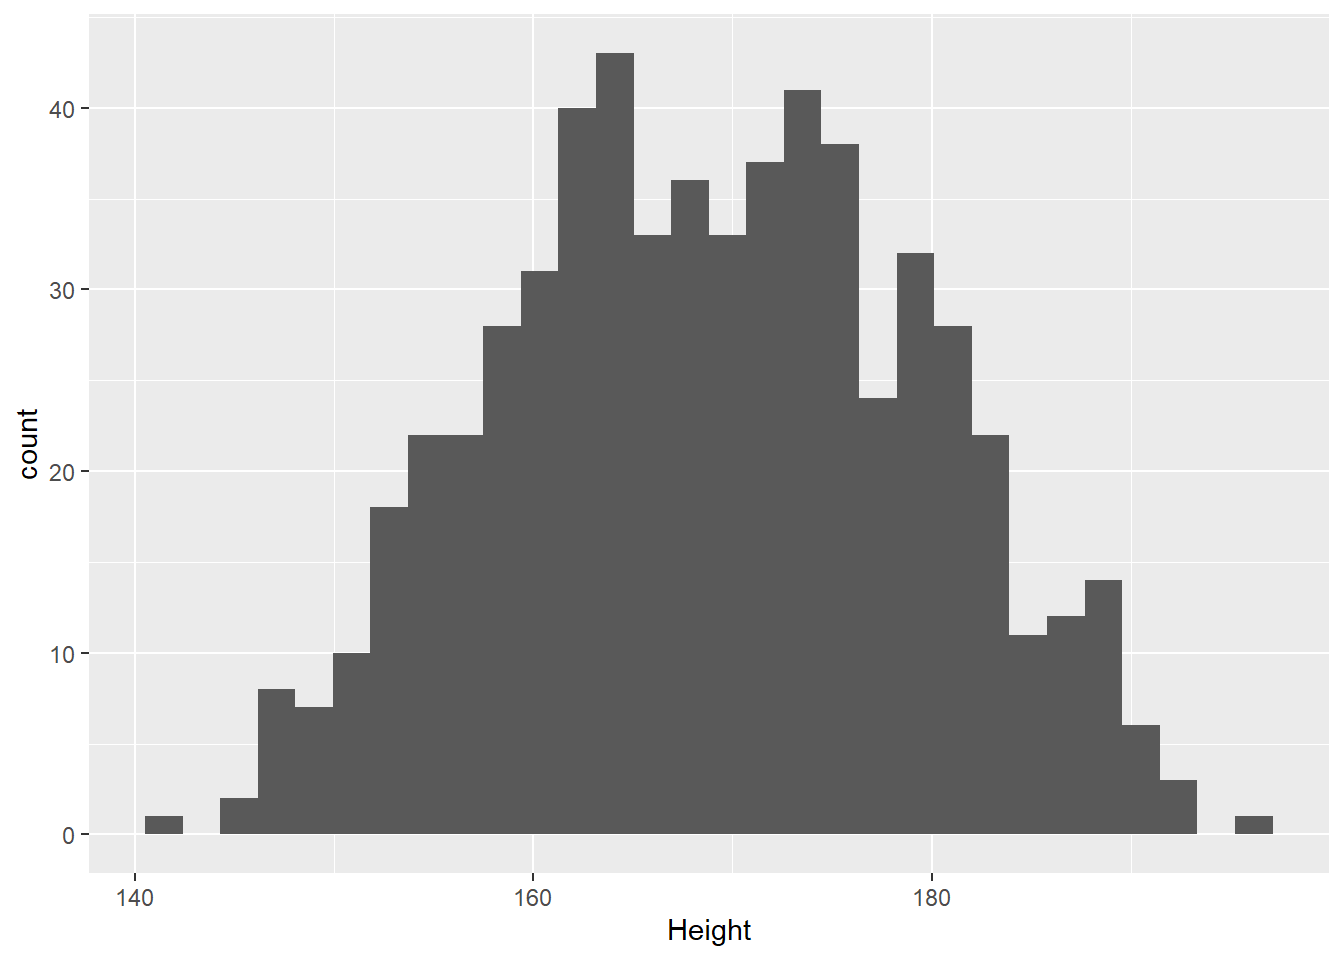
\includegraphics{431-notes_files/figure-latex/nh_dat3_heighthistogram-fig-1.pdf}

We can do several things to clean this up.

\begin{enumerate}
\def\labelenumi{\arabic{enumi}.}
\tightlist
\item
  We'll change the color of the lines for each bar of the histogram.
\item
  We'll change the fill inside each bar to make them stand out a bit more.
\item
  We'll add a title and relabel the horizontal (x) axis to include the units of measurement.
\item
  We'll avoid the warning by selecting a number of bins (we'll use 25 here) into which we'll group the heights before drawing the histogram.
\end{enumerate}

\begin{Shaded}
\begin{Highlighting}[]
\KeywordTok{ggplot}\NormalTok{(}\DataTypeTok{data =}\NormalTok{ nh_dat3, }\KeywordTok{aes}\NormalTok{(}\DataTypeTok{x =}\NormalTok{ Height)) }\OperatorTok{+}\StringTok{ }
\StringTok{    }\KeywordTok{geom_histogram}\NormalTok{(}\DataTypeTok{bins =} \DecValTok{25}\NormalTok{, }\DataTypeTok{col =} \StringTok{"yellow"}\NormalTok{, }\DataTypeTok{fill =} \StringTok{"blue"}\NormalTok{) }\OperatorTok{+}\StringTok{ }
\StringTok{    }\KeywordTok{labs}\NormalTok{(}\DataTypeTok{title =} \StringTok{"Height of NHANES subjects ages 21-79"}\NormalTok{,}
         \DataTypeTok{x =} \StringTok{"Height in cm."}\NormalTok{)}
\end{Highlighting}
\end{Shaded}

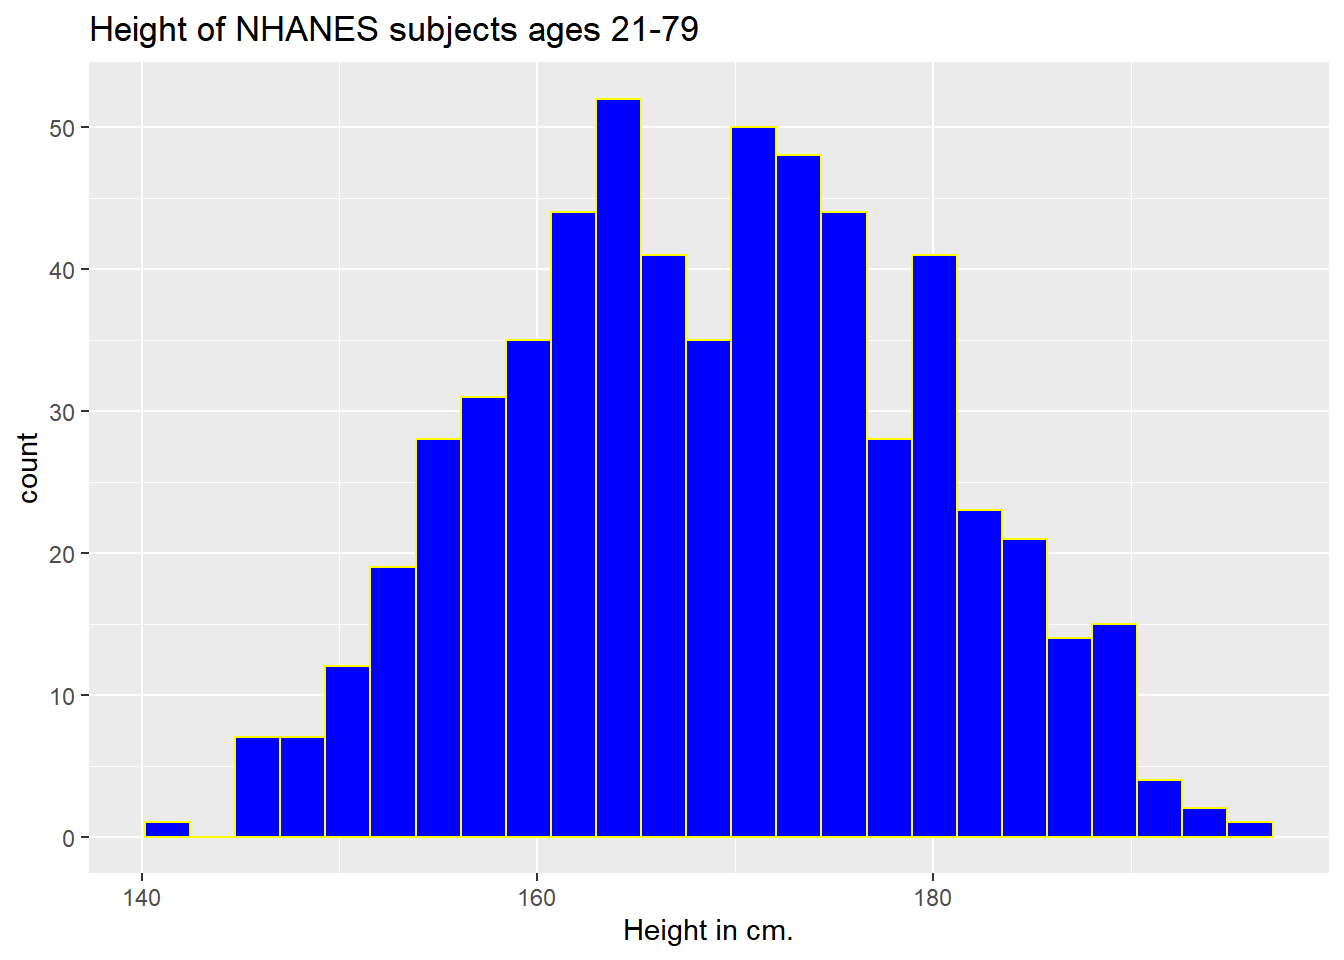
\includegraphics{431-notes_files/figure-latex/nh_dat3_heighthistogram2-fig-1.pdf}

\hypertarget{changing-a-histograms-fill-and-color}{%
\subsection{Changing a Histogram's Fill and Color}\label{changing-a-histograms-fill-and-color}}

The CWRU color guide (\url{https://case.edu/umc/our-brand/visual-guidelines/}) lists the HTML color schemes for CWRU blue and CWRU gray. Let's match that color scheme.

\begin{Shaded}
\begin{Highlighting}[]
\NormalTok{cwru.blue <-}\StringTok{ '#0a304e'}
\NormalTok{cwru.gray <-}\StringTok{ '#626262'}

\KeywordTok{ggplot}\NormalTok{(}\DataTypeTok{data =}\NormalTok{ nh_dat3, }\KeywordTok{aes}\NormalTok{(}\DataTypeTok{x =}\NormalTok{ Height)) }\OperatorTok{+}\StringTok{ }
\StringTok{    }\KeywordTok{geom_histogram}\NormalTok{(}\DataTypeTok{binwidth =} \DecValTok{2}\NormalTok{, }\DataTypeTok{col =}\NormalTok{ cwru.gray, }\DataTypeTok{fill =}\NormalTok{ cwru.blue) }\OperatorTok{+}\StringTok{ }
\StringTok{    }\KeywordTok{labs}\NormalTok{(}\DataTypeTok{title =} \StringTok{"Height of NHANES subjects ages 21-79"}\NormalTok{,}
         \DataTypeTok{x =} \StringTok{"Height in cm."}\NormalTok{) }\OperatorTok{+}
\StringTok{    }\KeywordTok{theme_bw}\NormalTok{()}
\end{Highlighting}
\end{Shaded}

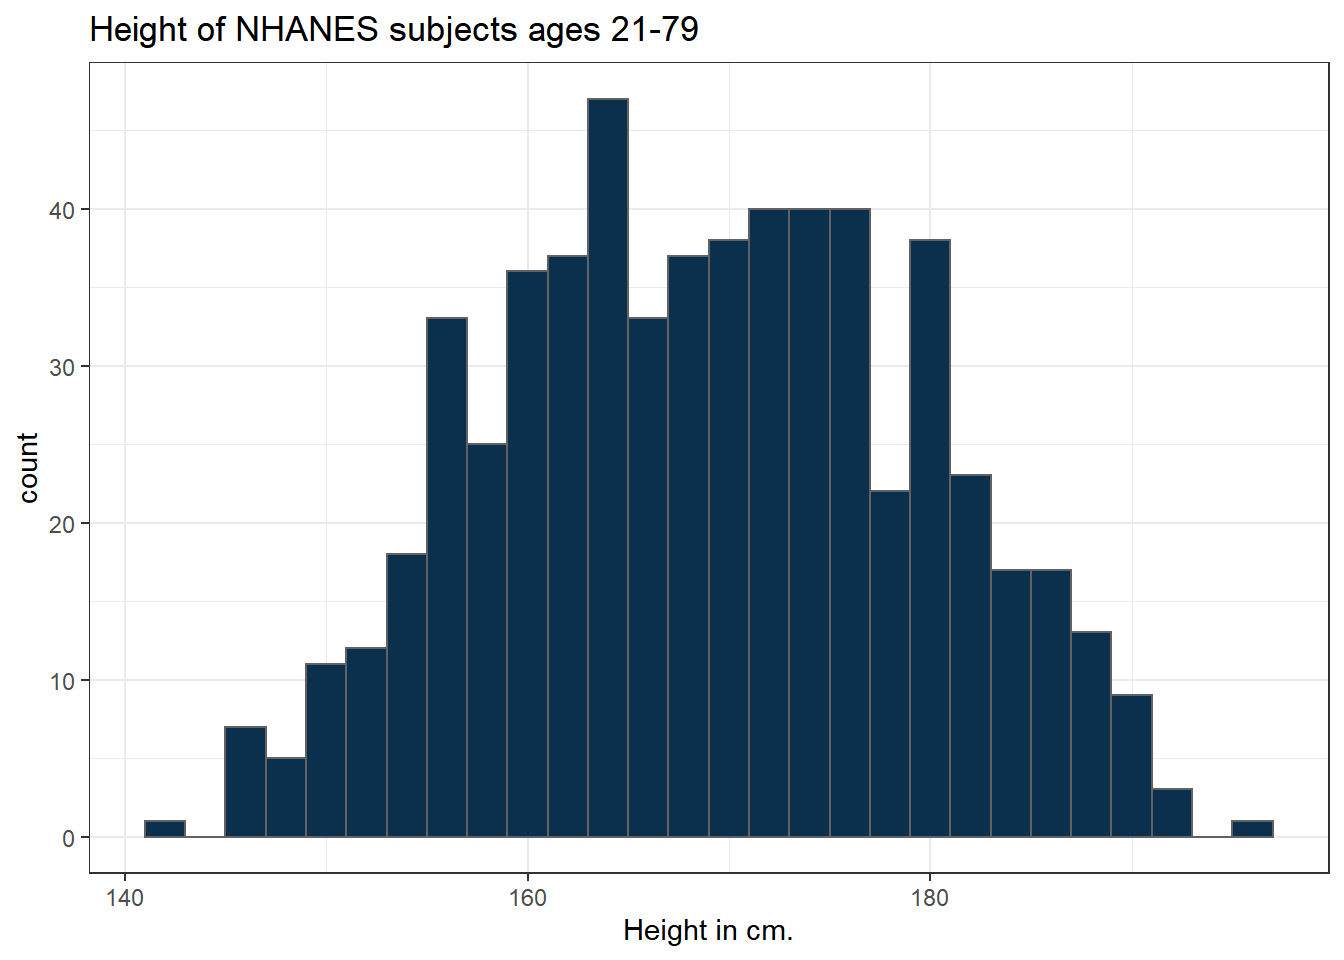
\includegraphics{431-notes_files/figure-latex/nh_dat3_histogramwithCWRUscheme-fig-1.pdf}

Note the other changes to the graph above.

\begin{enumerate}
\def\labelenumi{\arabic{enumi}.}
\tightlist
\item
  We changed the theme to replace the gray background.
\item
  We changed the bins for the histogram, to gather observations into groups of 2 cm. each.
\end{enumerate}

\hypertarget{height-and-sex}{%
\section{Height and Sex}\label{height-and-sex}}

\begin{Shaded}
\begin{Highlighting}[]
\KeywordTok{ggplot}\NormalTok{(}\DataTypeTok{data =}\NormalTok{ nh_dat3, }\KeywordTok{aes}\NormalTok{(}\DataTypeTok{x =}\NormalTok{ Sex, }\DataTypeTok{y =}\NormalTok{ Height, }\DataTypeTok{color =}\NormalTok{ Sex)) }\OperatorTok{+}\StringTok{ }
\StringTok{    }\KeywordTok{geom_point}\NormalTok{() }\OperatorTok{+}\StringTok{ }
\StringTok{    }\KeywordTok{labs}\NormalTok{(}\DataTypeTok{title =} \StringTok{"Height by Sex for NHANES subjects ages 21-79"}\NormalTok{,}
         \DataTypeTok{y =} \StringTok{"Height in cm."}\NormalTok{)}
\end{Highlighting}
\end{Shaded}

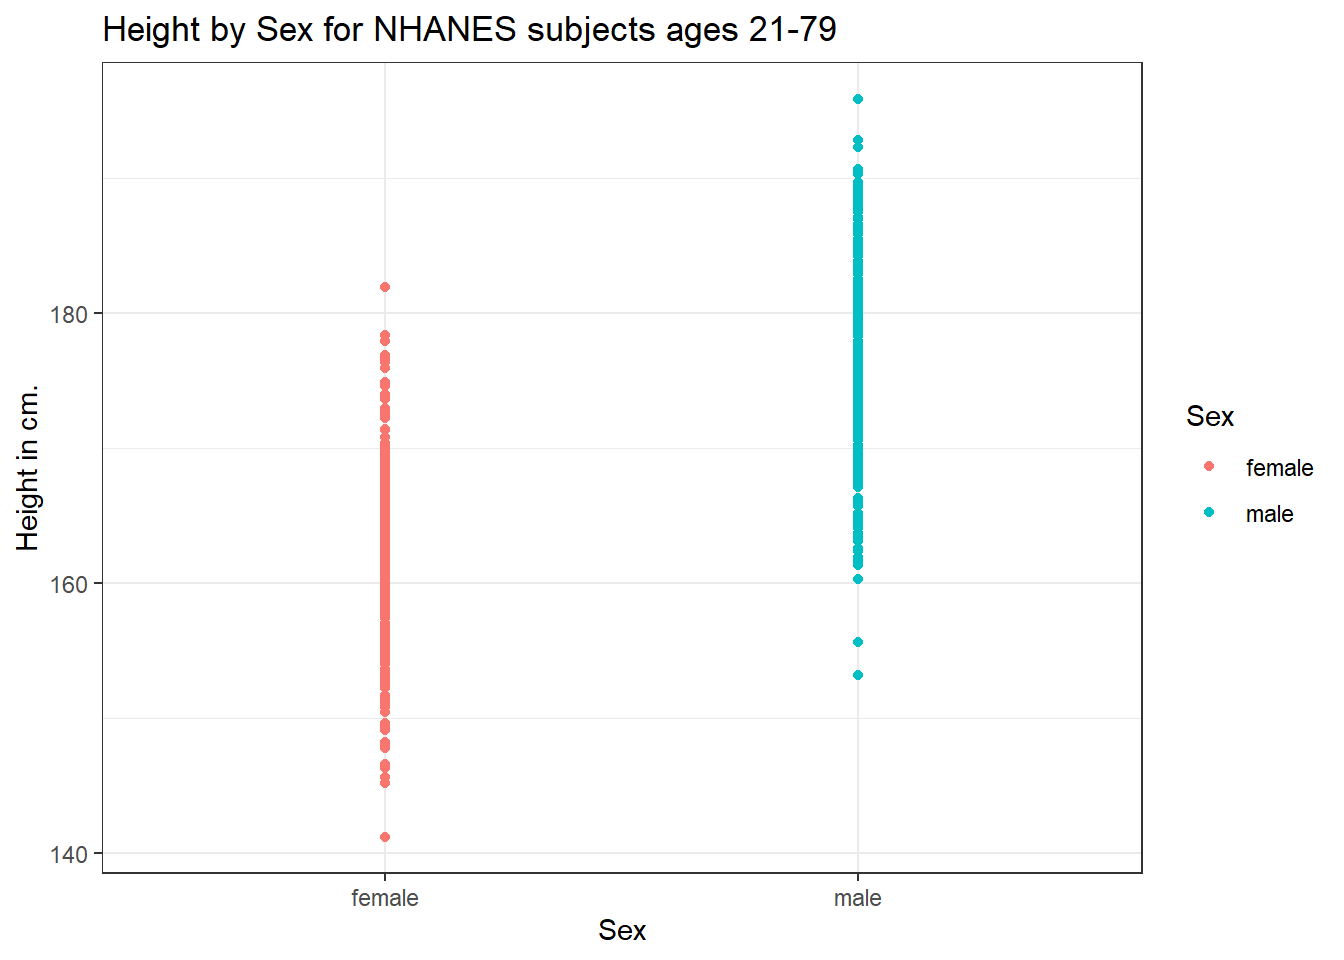
\includegraphics{431-notes_files/figure-latex/nh_dat3_heightbysex1-fig-1.pdf}

This plot isn't so useful. We can improve things a little by jittering the points horizontally, so that the overlap is reduced.

\begin{Shaded}
\begin{Highlighting}[]
\KeywordTok{ggplot}\NormalTok{(}\DataTypeTok{data =}\NormalTok{ nh_dat3, }\KeywordTok{aes}\NormalTok{(}\DataTypeTok{x =}\NormalTok{ Sex, }\DataTypeTok{y =}\NormalTok{ Height, }\DataTypeTok{color =}\NormalTok{ Sex)) }\OperatorTok{+}\StringTok{ }
\StringTok{    }\KeywordTok{geom_jitter}\NormalTok{(}\DataTypeTok{width =} \FloatTok{0.2}\NormalTok{) }\OperatorTok{+}\StringTok{ }
\StringTok{    }\KeywordTok{labs}\NormalTok{(}\DataTypeTok{title =} \StringTok{"Height by Sex (jittered) for NHANES subjects ages 21-79"}\NormalTok{,}
         \DataTypeTok{y =} \StringTok{"Height in cm."}\NormalTok{)}
\end{Highlighting}
\end{Shaded}

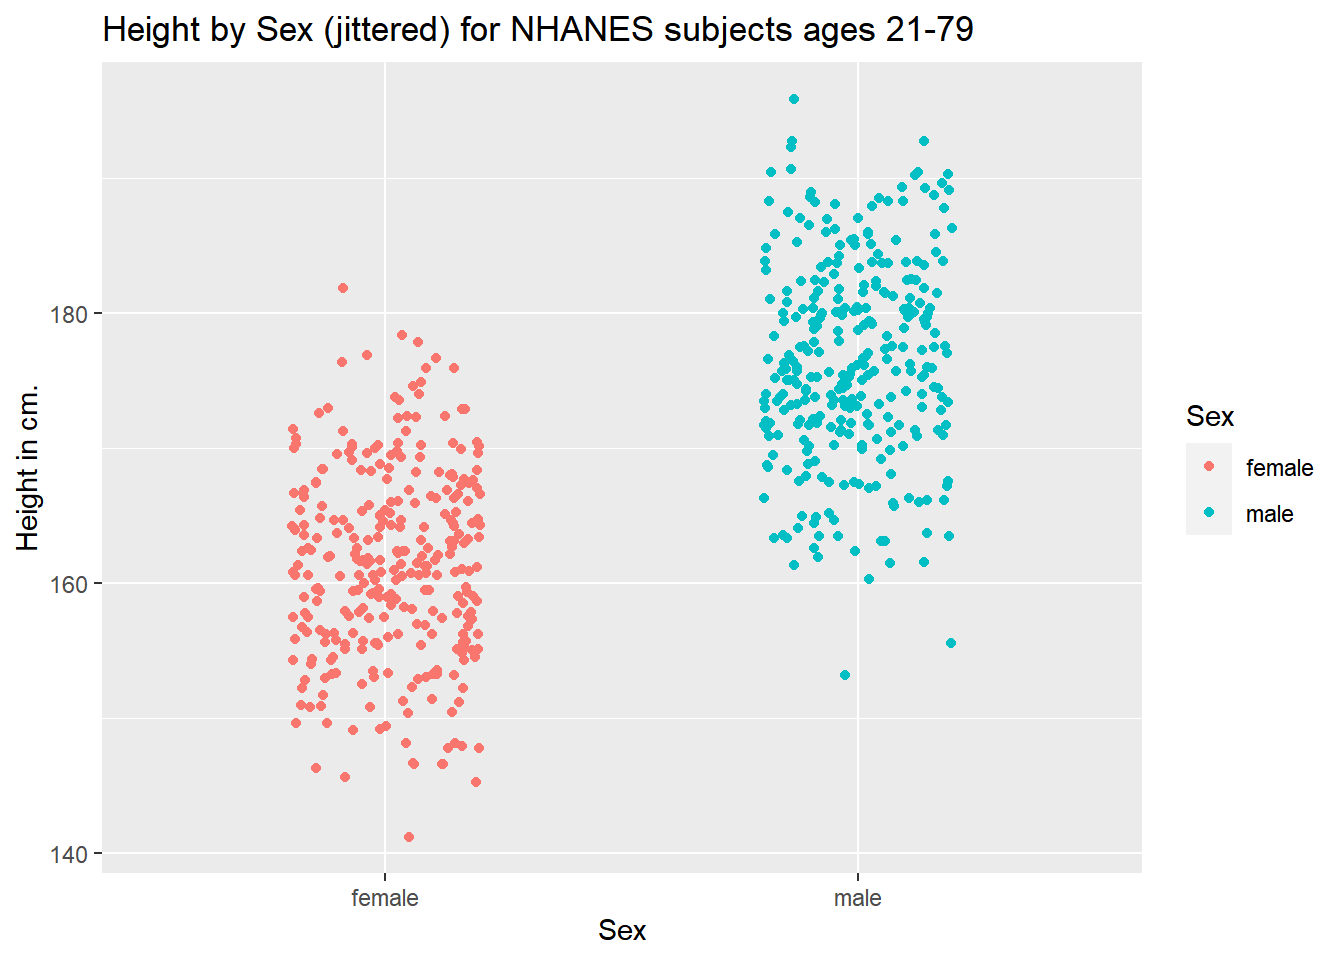
\includegraphics{431-notes_files/figure-latex/nh_dat3_heightbysex2-fig-1.pdf}

Perhaps it might be better to summarise the distribution in a different way. We might consider a boxplot of the data.

\hypertarget{a-boxplot-of-height-by-sex}{%
\subsection{A Boxplot of Height by Sex}\label{a-boxplot-of-height-by-sex}}

\begin{Shaded}
\begin{Highlighting}[]
\KeywordTok{ggplot}\NormalTok{(}\DataTypeTok{data =}\NormalTok{ nh_dat3, }\KeywordTok{aes}\NormalTok{(}\DataTypeTok{x =}\NormalTok{ Sex, }\DataTypeTok{y =}\NormalTok{ Height, }\DataTypeTok{fill =}\NormalTok{ Sex)) }\OperatorTok{+}\StringTok{ }
\StringTok{    }\KeywordTok{geom_boxplot}\NormalTok{() }\OperatorTok{+}\StringTok{ }
\StringTok{    }\KeywordTok{labs}\NormalTok{(}\DataTypeTok{title =} \StringTok{"Boxplot of Height by Sex for NHANES subjects ages 21-79"}\NormalTok{,}
         \DataTypeTok{y =} \StringTok{"Height in cm."}\NormalTok{)}
\end{Highlighting}
\end{Shaded}

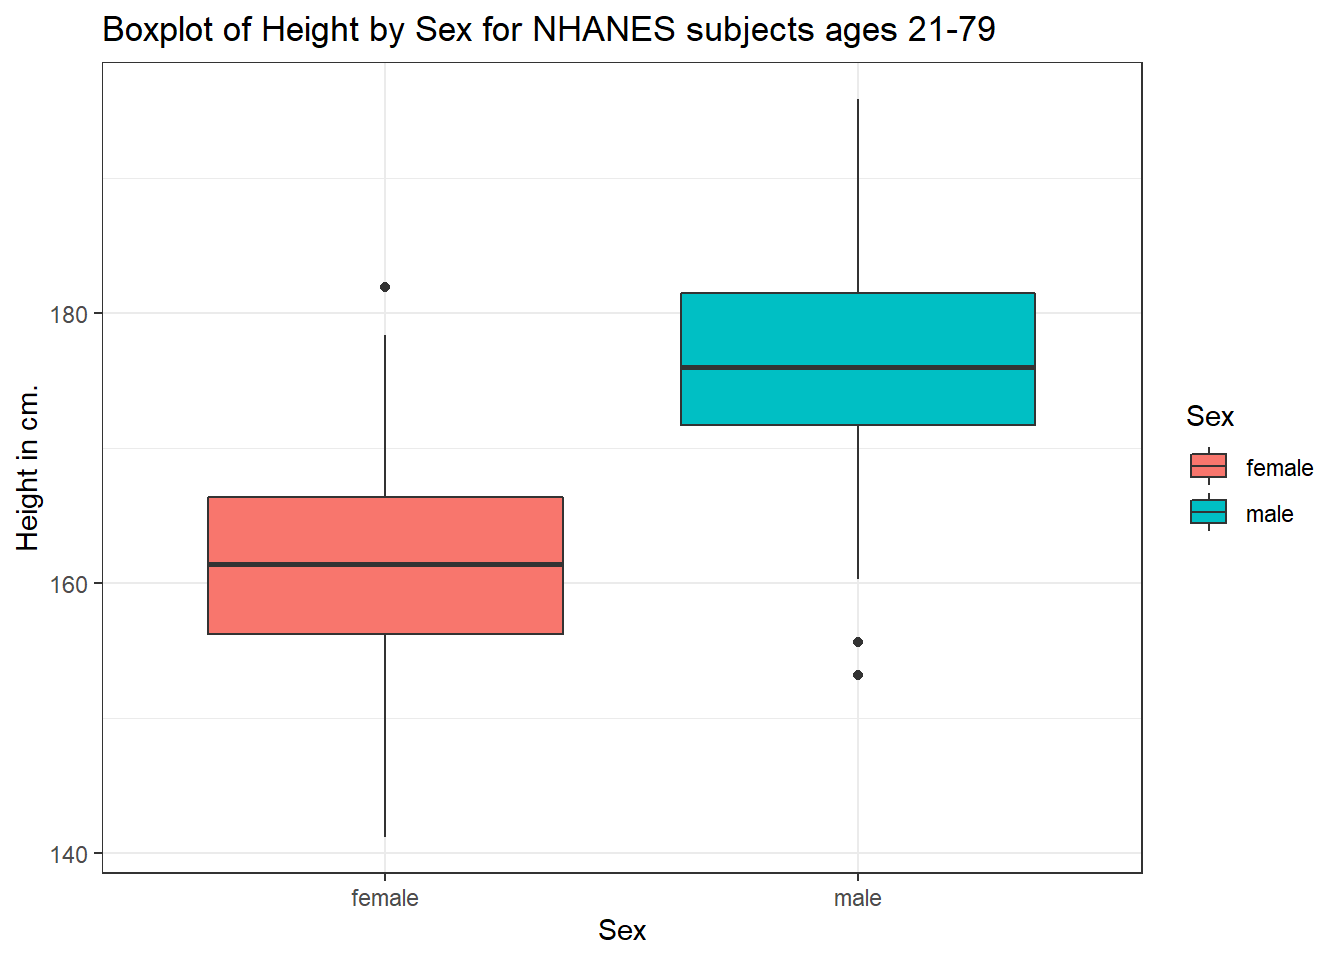
\includegraphics{431-notes_files/figure-latex/nh_dat3_heightbysexbox-fig-1.pdf}

Or perhaps we'd like to see a pair of histograms?

\hypertarget{histograms-of-height-by-sex}{%
\subsection{Histograms of Height by Sex}\label{histograms-of-height-by-sex}}

\begin{Shaded}
\begin{Highlighting}[]
\KeywordTok{ggplot}\NormalTok{(}\DataTypeTok{data =}\NormalTok{ nh_dat3, }\KeywordTok{aes}\NormalTok{(}\DataTypeTok{x =}\NormalTok{ Height, }\DataTypeTok{fill =}\NormalTok{ Sex)) }\OperatorTok{+}\StringTok{ }
\StringTok{    }\KeywordTok{geom_histogram}\NormalTok{(}\DataTypeTok{color =} \StringTok{"white"}\NormalTok{, }\DataTypeTok{bins =} \DecValTok{20}\NormalTok{) }\OperatorTok{+}\StringTok{ }
\StringTok{    }\KeywordTok{labs}\NormalTok{(}\DataTypeTok{title =} \StringTok{"Histogram of Height by Sex for NHANES subjects ages 21-79"}\NormalTok{,}
         \DataTypeTok{x =} \StringTok{"Height in cm."}\NormalTok{) }\OperatorTok{+}\StringTok{ }
\StringTok{    }\KeywordTok{facet_wrap}\NormalTok{(}\OperatorTok{~}\StringTok{ }\NormalTok{Sex)}
\end{Highlighting}
\end{Shaded}

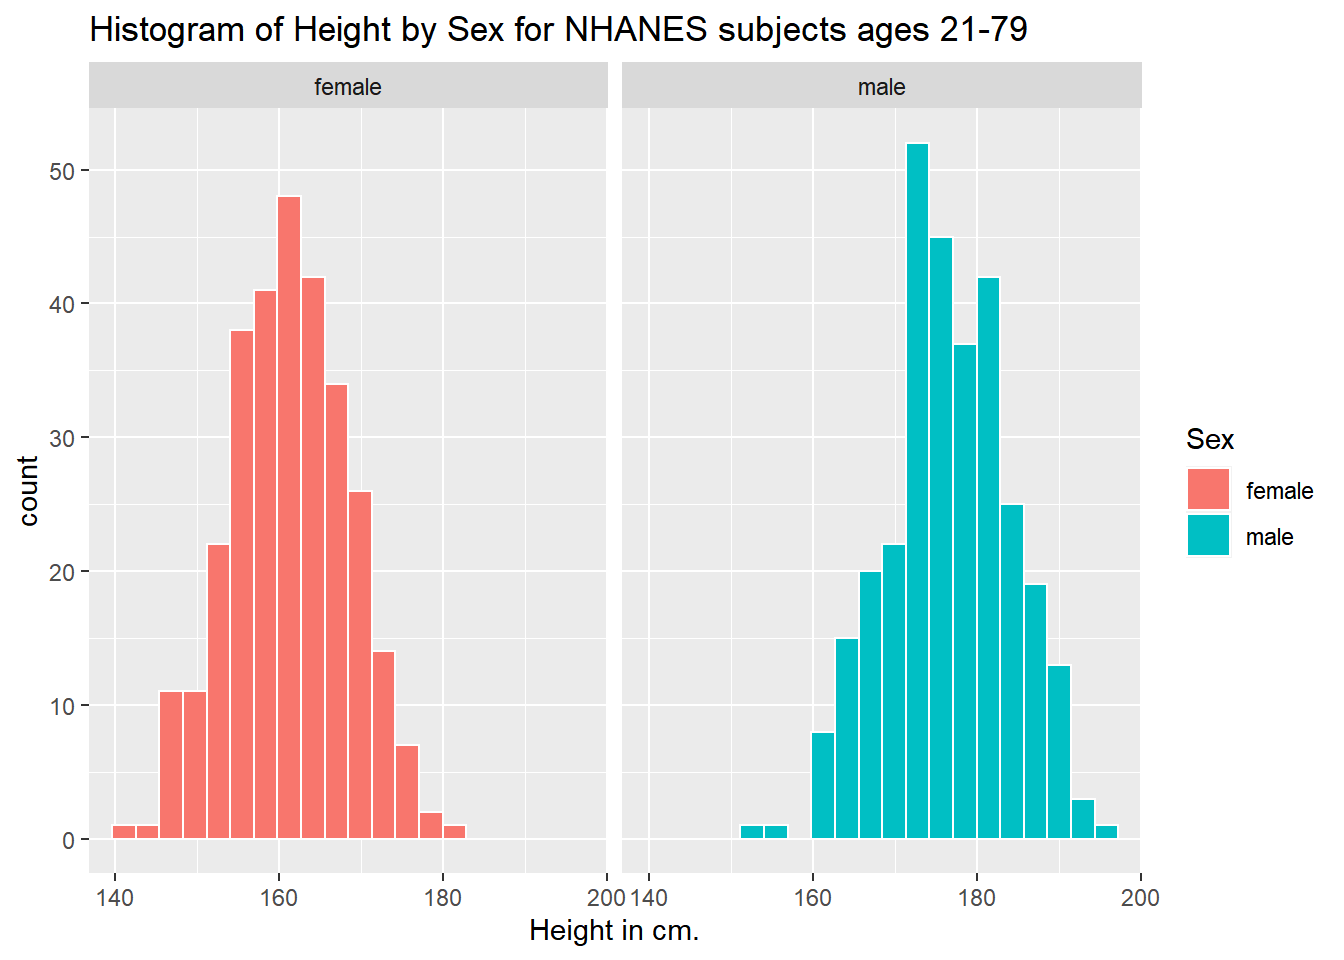
\includegraphics{431-notes_files/figure-latex/nh_dat3_heightbysexhist-fig-1.pdf}

Can we redraw these histograms so that they are a little more comparable, and to get rid of the unnecessary legend?

\begin{Shaded}
\begin{Highlighting}[]
\KeywordTok{ggplot}\NormalTok{(}\DataTypeTok{data =}\NormalTok{ nh_dat3, }\KeywordTok{aes}\NormalTok{(}\DataTypeTok{x =}\NormalTok{ Height, }\DataTypeTok{fill =}\NormalTok{ Sex)) }\OperatorTok{+}\StringTok{ }
\StringTok{    }\KeywordTok{geom_histogram}\NormalTok{(}\DataTypeTok{color =} \StringTok{"white"}\NormalTok{, }\DataTypeTok{bins =} \DecValTok{20}\NormalTok{) }\OperatorTok{+}\StringTok{ }
\StringTok{    }\KeywordTok{labs}\NormalTok{(}\DataTypeTok{title =} \StringTok{"Histogram of Height by Sex for NHANES subjects ages 21-79 (Revised)"}\NormalTok{,}
         \DataTypeTok{x =} \StringTok{"Height in cm."}\NormalTok{) }\OperatorTok{+}\StringTok{ }
\StringTok{    }\KeywordTok{guides}\NormalTok{(}\DataTypeTok{fill =} \OtherTok{FALSE}\NormalTok{) }\OperatorTok{+}
\StringTok{    }\KeywordTok{facet_grid}\NormalTok{(Sex }\OperatorTok{~}\StringTok{ }\NormalTok{.)}
\end{Highlighting}
\end{Shaded}

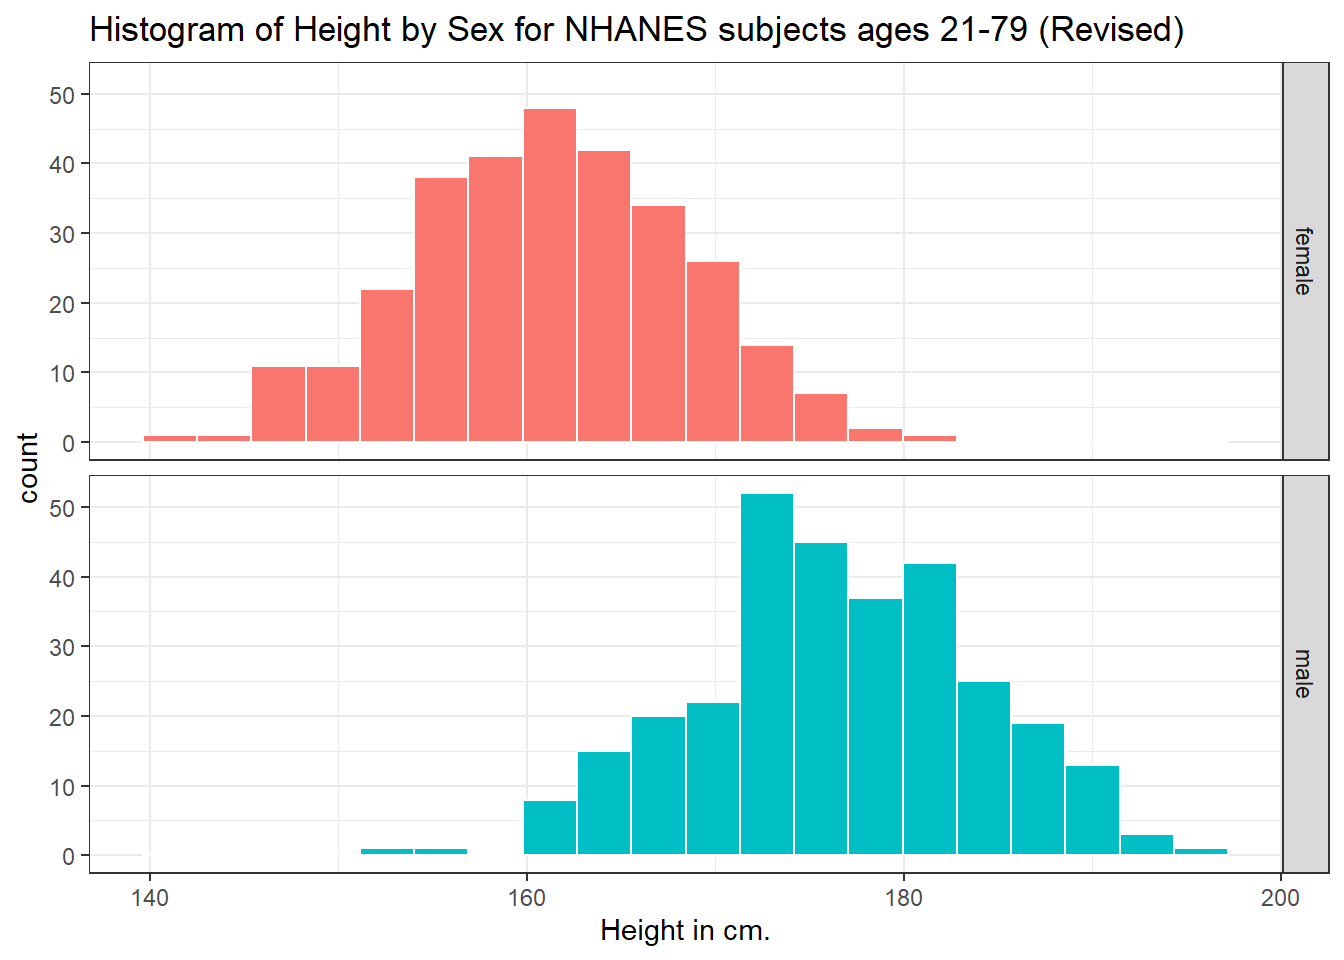
\includegraphics{431-notes_files/figure-latex/nh_dat3_heightbysexhist2-fig-1.pdf}

\hypertarget{looking-at-pulse-rate}{%
\section{Looking at Pulse Rate}\label{looking-at-pulse-rate}}

Let's look at a different outcome, the \emph{pulse rate} for our subjects.

Here's a histogram, again with CWRU colors, for the pulse rates in our sample.

\begin{Shaded}
\begin{Highlighting}[]
\KeywordTok{ggplot}\NormalTok{(}\DataTypeTok{data =}\NormalTok{ nh_dat3, }\KeywordTok{aes}\NormalTok{(}\DataTypeTok{x =}\NormalTok{ Pulse)) }\OperatorTok{+}\StringTok{ }
\StringTok{    }\KeywordTok{geom_histogram}\NormalTok{(}\DataTypeTok{binwidth =} \DecValTok{1}\NormalTok{, }\DataTypeTok{fill =}\NormalTok{ cwru.blue, }\DataTypeTok{col =}\NormalTok{ cwru.gray) }\OperatorTok{+}\StringTok{ }
\StringTok{    }\KeywordTok{labs}\NormalTok{(}\DataTypeTok{title =} \StringTok{"Histogram of Pulse Rate: NHANES subjects ages 21-79"}\NormalTok{,}
         \DataTypeTok{x =} \StringTok{"Pulse Rate (beats per minute)"}\NormalTok{)}
\end{Highlighting}
\end{Shaded}

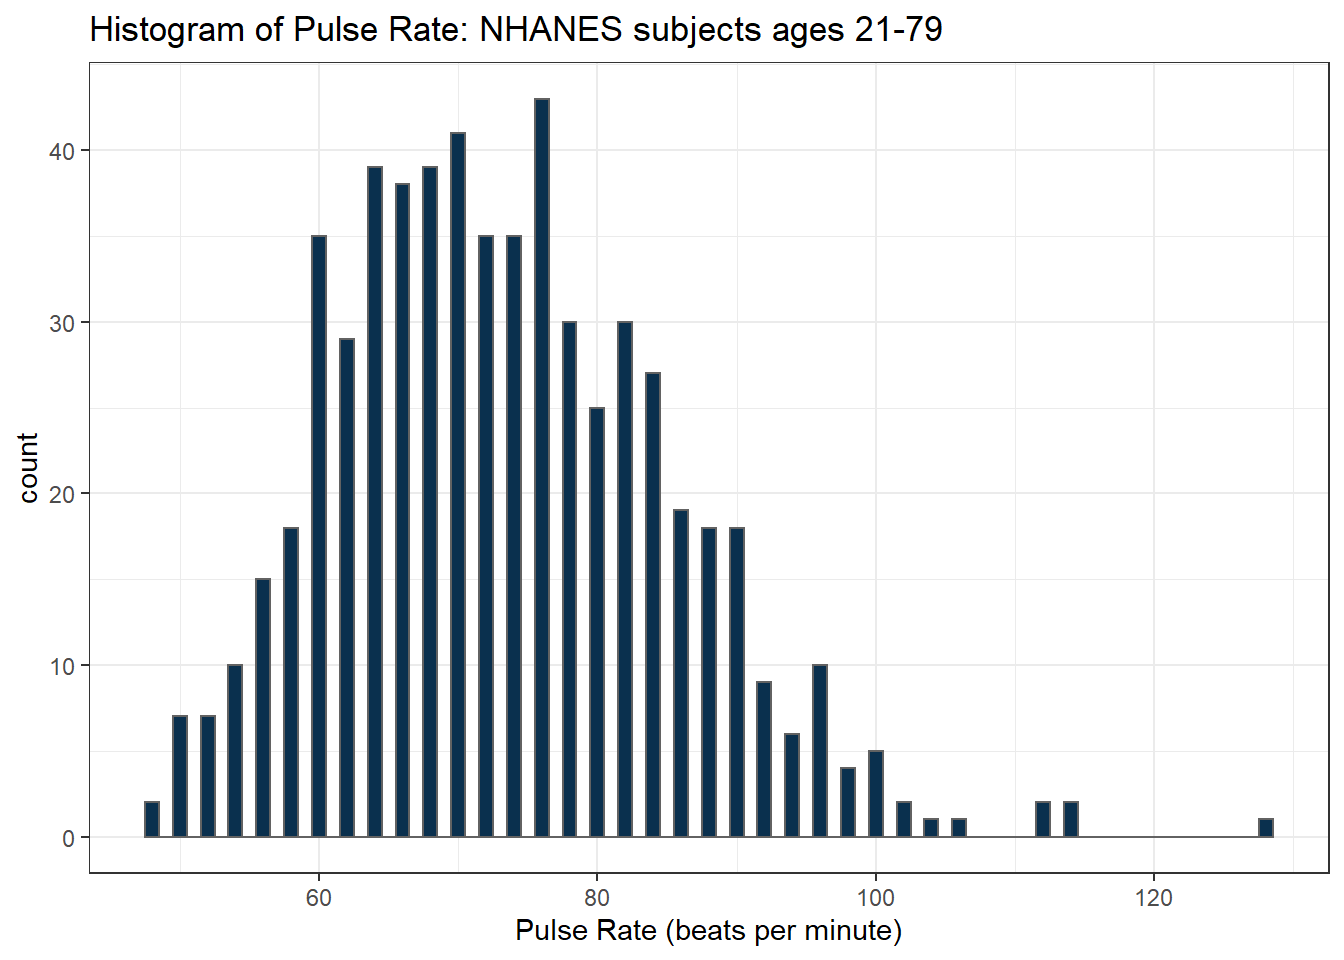
\includegraphics{431-notes_files/figure-latex/nh_dat3_pulse_histbin1-fig-1.pdf}

Suppose we instead bin up groups of 5 beats per minute together as we plot the Pulse rates.

\begin{Shaded}
\begin{Highlighting}[]
\KeywordTok{ggplot}\NormalTok{(}\DataTypeTok{data =}\NormalTok{ nh_dat3, }\KeywordTok{aes}\NormalTok{(}\DataTypeTok{x =}\NormalTok{ Pulse)) }\OperatorTok{+}\StringTok{ }
\StringTok{    }\KeywordTok{geom_histogram}\NormalTok{(}\DataTypeTok{binwidth =} \DecValTok{5}\NormalTok{, }\DataTypeTok{fill =}\NormalTok{ cwru.blue, }\DataTypeTok{col =}\NormalTok{ cwru.gray) }\OperatorTok{+}\StringTok{ }
\StringTok{    }\KeywordTok{labs}\NormalTok{(}\DataTypeTok{title =} \StringTok{"Histogram of Pulse Rate: NHANES subjects ages 21-79"}\NormalTok{,}
         \DataTypeTok{x =} \StringTok{"Pulse Rate (beats per minute)"}\NormalTok{)}
\end{Highlighting}
\end{Shaded}

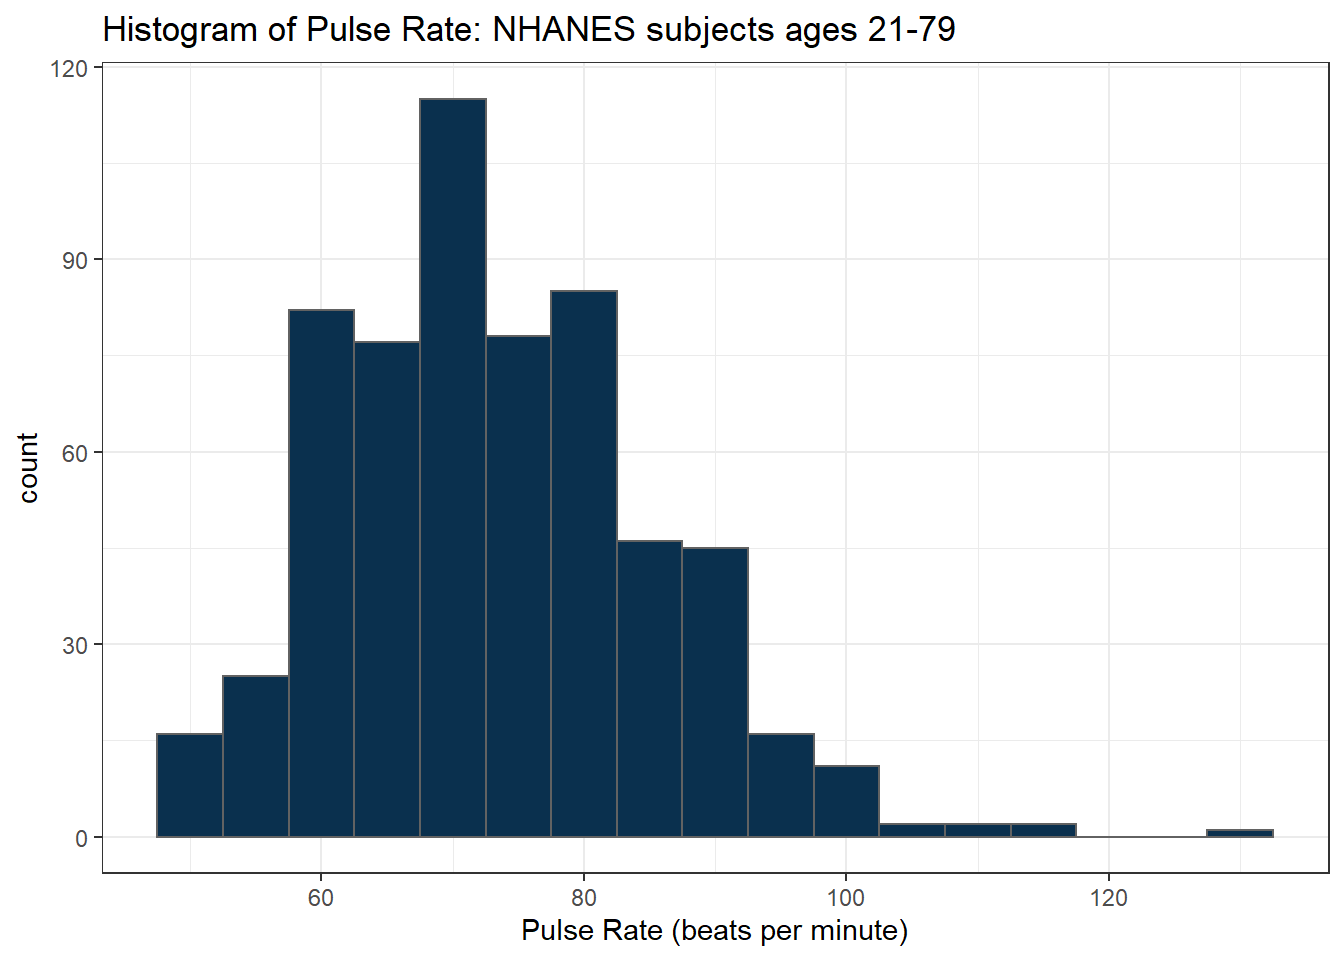
\includegraphics{431-notes_files/figure-latex/nh_dat3_pulse_histbin5-fig-1.pdf}

Which is the more useful representation will depend a lot on what questions you're trying to answer.

\hypertarget{pulse-rate-and-physical-activity}{%
\subsection{Pulse Rate and Physical Activity}\label{pulse-rate-and-physical-activity}}

We can also split up our data into groups based on whether the subjects are physically active. Let's try a boxplot.

\begin{Shaded}
\begin{Highlighting}[]
\KeywordTok{ggplot}\NormalTok{(}\DataTypeTok{data =}\NormalTok{ nh_dat3, }\KeywordTok{aes}\NormalTok{(}\DataTypeTok{y =}\NormalTok{ Pulse, }\DataTypeTok{x =}\NormalTok{ PhysActive, }\DataTypeTok{fill =}\NormalTok{ PhysActive)) }\OperatorTok{+}\StringTok{ }
\StringTok{    }\KeywordTok{geom_boxplot}\NormalTok{() }\OperatorTok{+}\StringTok{ }
\StringTok{    }\KeywordTok{labs}\NormalTok{(}\DataTypeTok{title =} \StringTok{"Pulse Rate by Physical Activity Status for NHANES ages 21-79"}\NormalTok{)}
\end{Highlighting}
\end{Shaded}

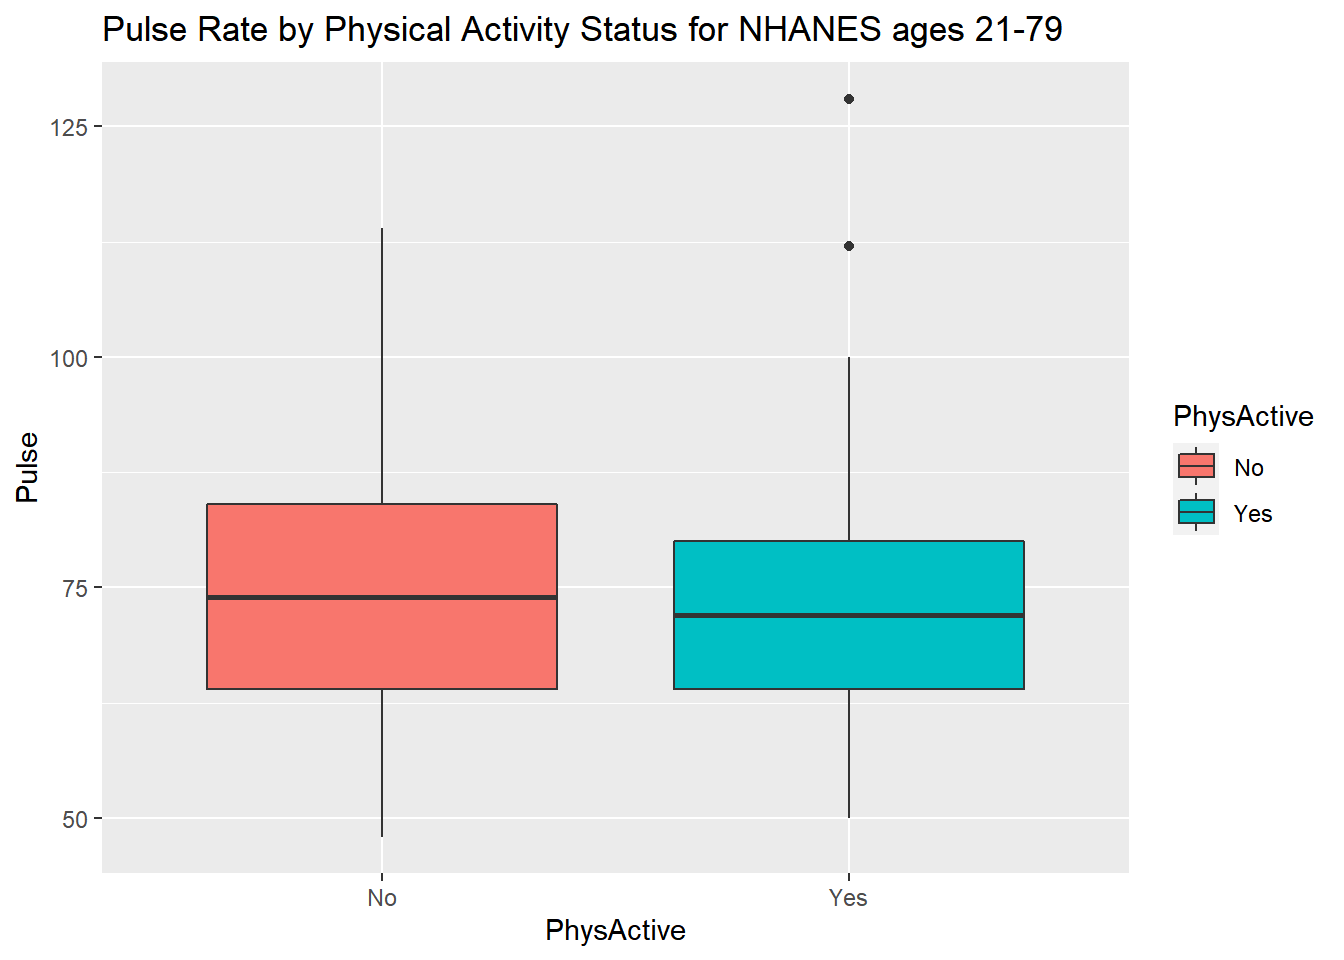
\includegraphics{431-notes_files/figure-latex/nh_dat3_pulse_by_activity_box-fig-1.pdf}

As an accompanying numerical summary, we might ask how many people fall into each of these \texttt{PhysActive} categories, and what is their ``average'' \texttt{Pulse} rate.

\begin{Shaded}
\begin{Highlighting}[]
\NormalTok{nh_dat3 }\OperatorTok
\StringTok{    }\KeywordTok{group_by}\NormalTok{(PhysActive) }\OperatorTok
\StringTok{    }\KeywordTok{summarise}\NormalTok{(}\DataTypeTok{count =} \KeywordTok{n}\NormalTok{(), }\KeywordTok{mean}\NormalTok{(Pulse), }\KeywordTok{median}\NormalTok{(Pulse)) }\OperatorTok
\StringTok{    }\NormalTok{knitr}\OperatorTok{::}\KeywordTok{kable}\NormalTok{(}\DataTypeTok{digits =} \DecValTok{2}\NormalTok{) }
\end{Highlighting}
\end{Shaded}

\begin{verbatim}
`summarise()` ungrouping output (override with `.groups` argument)
\end{verbatim}

\begin{tabular}{l|r|r|r}
\hline
PhysActive & count & mean(Pulse) & median(Pulse)\\
\hline
No & 293 & 74.21 & 74\\
\hline
Yes & 310 & 72.37 & 72\\
\hline
\end{tabular}

The \texttt{knitr::kable(digits\ =\ 2)} piece of this command tells R Markdown to generate a table with some attractive formatting, and rounding any decimals to two figures.

\hypertarget{pulse-by-sleeping-trouble}{%
\subsection{Pulse by Sleeping Trouble}\label{pulse-by-sleeping-trouble}}

\begin{Shaded}
\begin{Highlighting}[]
\KeywordTok{ggplot}\NormalTok{(}\DataTypeTok{data =}\NormalTok{ nh_dat3, }\KeywordTok{aes}\NormalTok{(}\DataTypeTok{x =}\NormalTok{ Pulse, }\DataTypeTok{fill =}\NormalTok{ SleepTrouble)) }\OperatorTok{+}\StringTok{ }
\StringTok{    }\KeywordTok{geom_histogram}\NormalTok{(}\DataTypeTok{color =} \StringTok{"white"}\NormalTok{, }\DataTypeTok{bins =} \DecValTok{20}\NormalTok{) }\OperatorTok{+}\StringTok{ }
\StringTok{    }\KeywordTok{labs}\NormalTok{(}\DataTypeTok{title =} \StringTok{"Histogram of Pulse Rate by Sleep Trouble for NHANES subjects ages 21-79"}\NormalTok{,}
         \DataTypeTok{x =} \StringTok{"Pulse Rate (beats per minute)"}\NormalTok{) }\OperatorTok{+}\StringTok{ }
\StringTok{    }\KeywordTok{guides}\NormalTok{(}\DataTypeTok{fill =} \OtherTok{FALSE}\NormalTok{) }\OperatorTok{+}
\StringTok{    }\KeywordTok{facet_grid}\NormalTok{(SleepTrouble }\OperatorTok{~}\StringTok{ }\NormalTok{., }\DataTypeTok{labeller =} \StringTok{"label_both"}\NormalTok{)}
\end{Highlighting}
\end{Shaded}

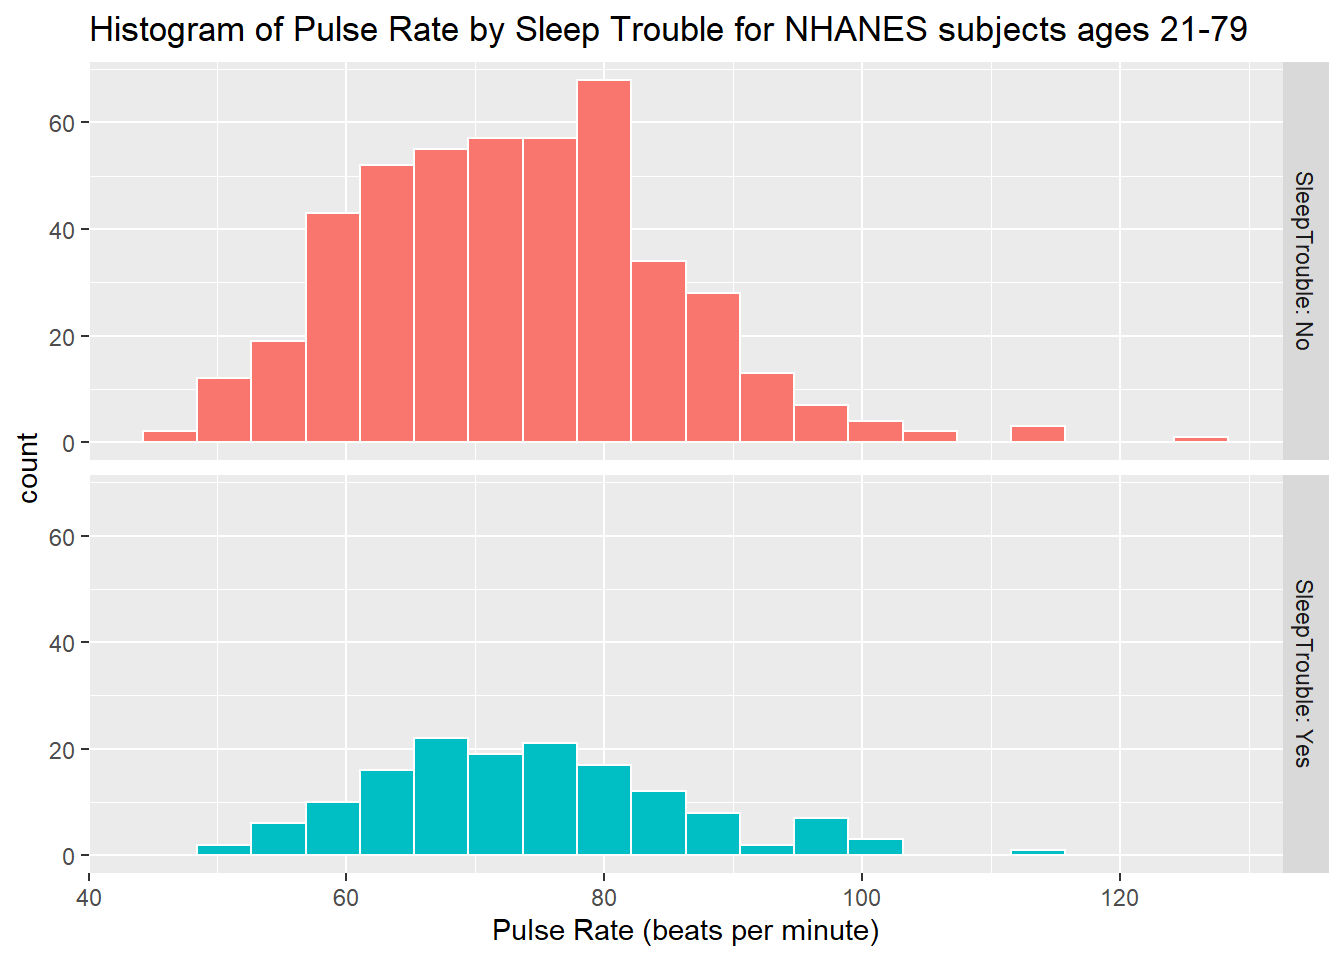
\includegraphics{431-notes_files/figure-latex/nh_dat3_pulse_by_sleep_histbin1-fig-1.pdf}

How many people fall into each of these \texttt{SleepTrouble} categories, and what is their ``average'' Pulse rate?

\begin{Shaded}
\begin{Highlighting}[]
\NormalTok{nh_dat3 }\OperatorTok
\StringTok{    }\KeywordTok{group_by}\NormalTok{(SleepTrouble) }\OperatorTok
\StringTok{    }\KeywordTok{summarise}\NormalTok{(}\DataTypeTok{count =} \KeywordTok{n}\NormalTok{(), }\KeywordTok{mean}\NormalTok{(Pulse), }\KeywordTok{median}\NormalTok{(Pulse)) }\OperatorTok
\StringTok{    }\NormalTok{knitr}\OperatorTok{::}\KeywordTok{kable}\NormalTok{(}\DataTypeTok{digits =} \DecValTok{2}\NormalTok{) }
\end{Highlighting}
\end{Shaded}

\begin{verbatim}
`summarise()` ungrouping output (override with `.groups` argument)
\end{verbatim}

\begin{tabular}{l|r|r|r}
\hline
SleepTrouble & count & mean(Pulse) & median(Pulse)\\
\hline
No & 457 & 73.05 & 72\\
\hline
Yes & 146 & 73.96 & 72\\
\hline
\end{tabular}

\hypertarget{pulse-and-healthgen}{%
\subsection{Pulse and HealthGen}\label{pulse-and-healthgen}}

We can compare the distribution of Pulse rate across groups by the subject's self-reported overall health (\texttt{HealthGen}), as well.

\begin{Shaded}
\begin{Highlighting}[]
\KeywordTok{ggplot}\NormalTok{(}\DataTypeTok{data =}\NormalTok{ nh_dat3, }\KeywordTok{aes}\NormalTok{(}\DataTypeTok{x =}\NormalTok{ HealthGen, }\DataTypeTok{y =}\NormalTok{ Pulse, }\DataTypeTok{fill =}\NormalTok{ HealthGen)) }\OperatorTok{+}\StringTok{ }
\StringTok{    }\KeywordTok{geom_boxplot}\NormalTok{() }\OperatorTok{+}
\StringTok{    }\KeywordTok{labs}\NormalTok{(}\DataTypeTok{title =} \StringTok{"Pulse by Self-Reported Overall Health for NHANES ages 21-79"}\NormalTok{,}
         \DataTypeTok{x =} \StringTok{"Pulse Rate"}\NormalTok{) }\OperatorTok{+}\StringTok{ }
\StringTok{    }\KeywordTok{guides}\NormalTok{(}\DataTypeTok{fill =} \OtherTok{FALSE}\NormalTok{) }
\end{Highlighting}
\end{Shaded}

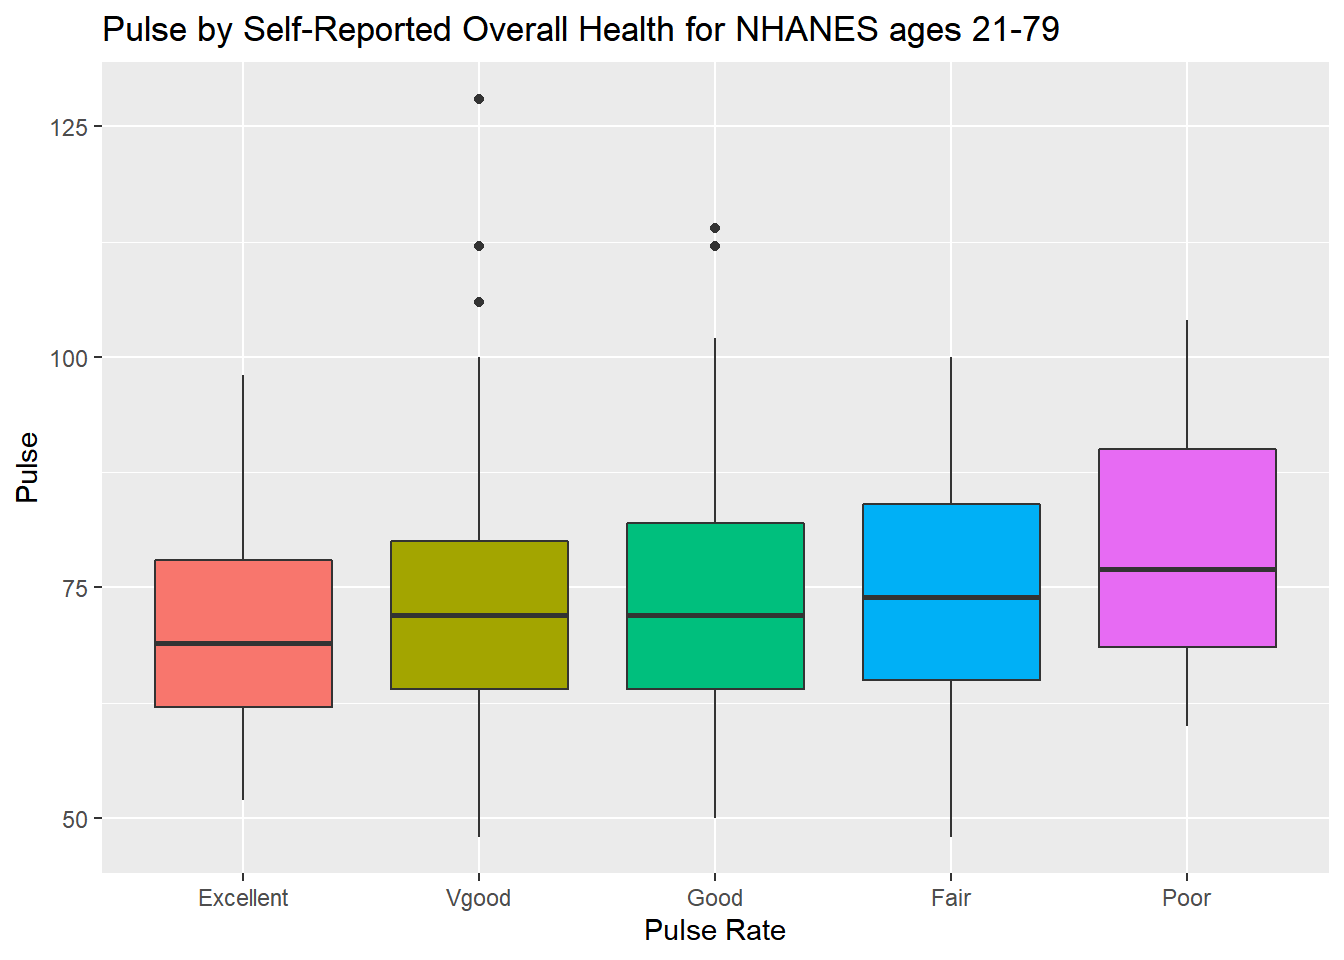
\includegraphics{431-notes_files/figure-latex/nh_dat3_pulsebyhealthgen1-fig-1.pdf}

How many people fall into each of these \texttt{HealthGen} categories, and what is their ``average'' Pulse rate?

\begin{Shaded}
\begin{Highlighting}[]
\NormalTok{nh_dat3 }\OperatorTok
\StringTok{    }\KeywordTok{group_by}\NormalTok{(HealthGen) }\OperatorTok
\StringTok{    }\KeywordTok{summarise}\NormalTok{(}\DataTypeTok{count =} \KeywordTok{n}\NormalTok{(), }\KeywordTok{mean}\NormalTok{(Pulse), }\KeywordTok{median}\NormalTok{(Pulse)) }\OperatorTok
\StringTok{    }\NormalTok{knitr}\OperatorTok{::}\KeywordTok{kable}\NormalTok{(}\DataTypeTok{digits =} \DecValTok{2}\NormalTok{) }
\end{Highlighting}
\end{Shaded}

\begin{verbatim}
`summarise()` ungrouping output (override with `.groups` argument)
\end{verbatim}

\begin{tabular}{l|r|r|r}
\hline
HealthGen & count & mean(Pulse) & median(Pulse)\\
\hline
Excellent & 64 & 69.97 & 69\\
\hline
Vgood & 196 & 72.81 & 72\\
\hline
Good & 238 & 73.66 & 72\\
\hline
Fair & 83 & 74.22 & 74\\
\hline
Poor & 22 & 79.09 & 77\\
\hline
\end{tabular}

\hypertarget{pulse-rate-and-systolic-blood-pressure}{%
\subsection{Pulse Rate and Systolic Blood Pressure}\label{pulse-rate-and-systolic-blood-pressure}}

\begin{Shaded}
\begin{Highlighting}[]
\KeywordTok{ggplot}\NormalTok{(}\DataTypeTok{data =}\NormalTok{ nh_dat3, }\KeywordTok{aes}\NormalTok{(}\DataTypeTok{x =}\NormalTok{ SBP, }\DataTypeTok{y =}\NormalTok{ Pulse)) }\OperatorTok{+}
\StringTok{    }\KeywordTok{geom_point}\NormalTok{() }\OperatorTok{+}
\StringTok{    }\KeywordTok{geom_smooth}\NormalTok{(}\DataTypeTok{method =} \StringTok{"loess"}\NormalTok{) }\OperatorTok{+}
\StringTok{    }\KeywordTok{labs}\NormalTok{(}\DataTypeTok{title =} \StringTok{"SBP vs. Pulse rate for NHANES subjects, ages 21-79"}\NormalTok{)}
\end{Highlighting}
\end{Shaded}

\begin{verbatim}
`geom_smooth()` using formula 'y ~ x'
\end{verbatim}

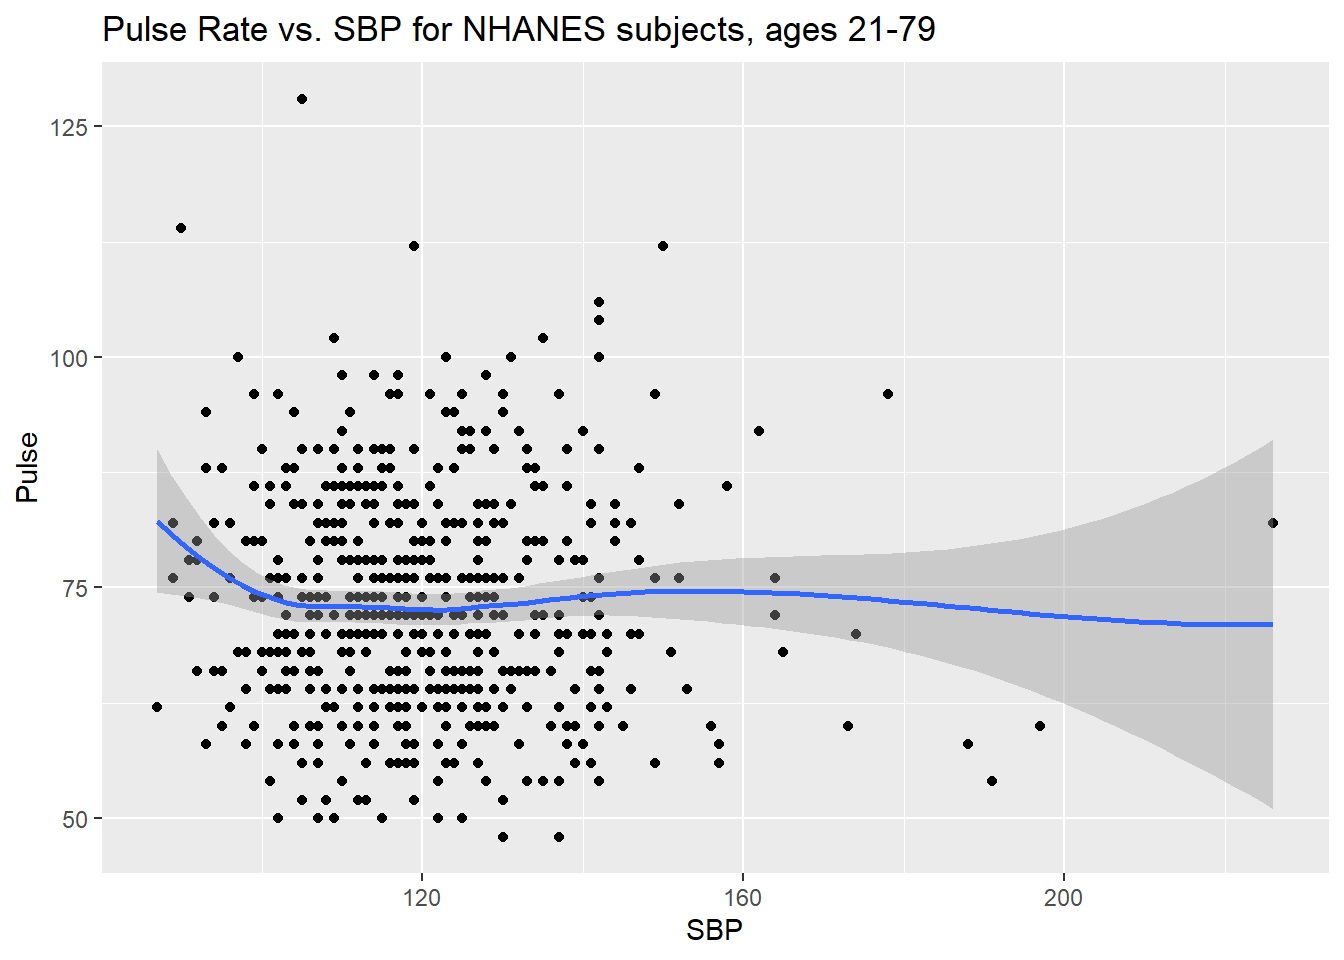
\includegraphics{431-notes_files/figure-latex/nh_dat3_pulsevssbp-fig-1.pdf}

\hypertarget{sleep-troubls-vs.-no-sleep-trouble}{%
\subsection{Sleep Troubls vs.~No Sleep Trouble?}\label{sleep-troubls-vs.-no-sleep-trouble}}

Could we see whether subjects who have described \texttt{SleepTrouble} show different SBP-pulse rate patterns than the subjects who haven't?

\begin{itemize}
\tightlist
\item
  Let's try doing this by changing the shape \emph{and} the color of the points based on \texttt{SleepTrouble}.
\end{itemize}

\begin{Shaded}
\begin{Highlighting}[]
\KeywordTok{ggplot}\NormalTok{(}\DataTypeTok{data =}\NormalTok{ nh_dat3, }
       \KeywordTok{aes}\NormalTok{(}\DataTypeTok{x =}\NormalTok{ SBP, }\DataTypeTok{y =}\NormalTok{ Pulse, }
           \DataTypeTok{color =}\NormalTok{ SleepTrouble, }\DataTypeTok{shape =}\NormalTok{ SleepTrouble)) }\OperatorTok{+}
\StringTok{    }\KeywordTok{geom_point}\NormalTok{() }\OperatorTok{+}
\StringTok{    }\KeywordTok{geom_smooth}\NormalTok{(}\DataTypeTok{method =} \StringTok{"loess"}\NormalTok{) }\OperatorTok{+}
\StringTok{    }\KeywordTok{labs}\NormalTok{(}\DataTypeTok{title =} \StringTok{"SBP vs. Pulse rate for NHANES subjects, ages 21-79"}\NormalTok{)}
\end{Highlighting}
\end{Shaded}

\begin{verbatim}
`geom_smooth()` using formula 'y ~ x'
\end{verbatim}

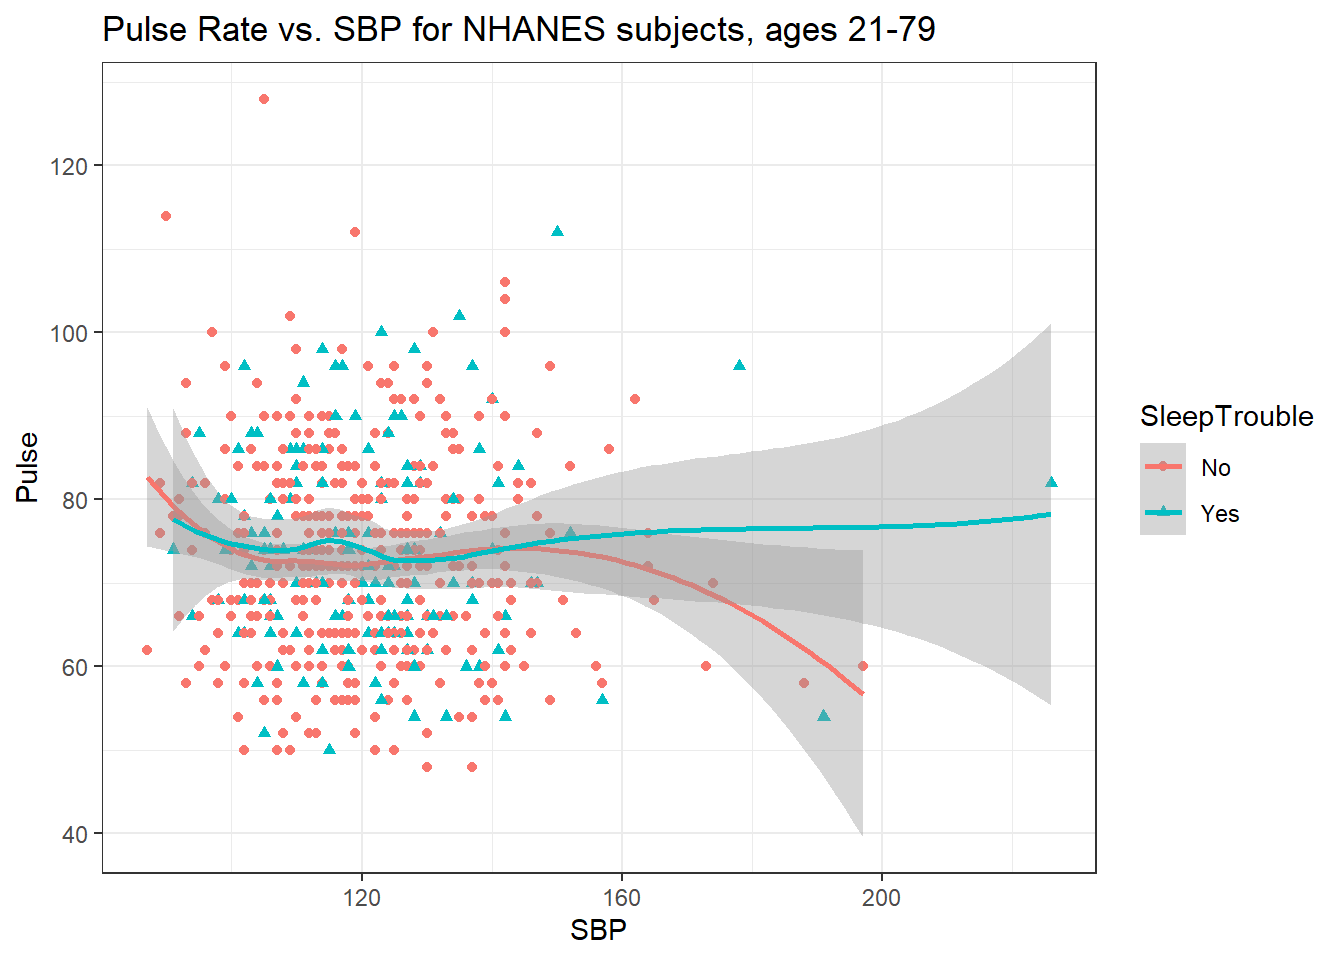
\includegraphics{431-notes_files/figure-latex/nh_dat3_sbpvspulsewithsleep-fig-1.pdf}

This plot might be easier to interpret if we faceted by \texttt{SleepTrouble}, as well.

\begin{Shaded}
\begin{Highlighting}[]
\KeywordTok{ggplot}\NormalTok{(}\DataTypeTok{data =}\NormalTok{ nh_dat3, }
       \KeywordTok{aes}\NormalTok{(}\DataTypeTok{x =}\NormalTok{ SBP, }\DataTypeTok{y =}\NormalTok{ Pulse, }
           \DataTypeTok{color =}\NormalTok{ SleepTrouble, }\DataTypeTok{shape =}\NormalTok{ SleepTrouble)) }\OperatorTok{+}
\StringTok{    }\KeywordTok{geom_point}\NormalTok{() }\OperatorTok{+}
\StringTok{    }\KeywordTok{geom_smooth}\NormalTok{(}\DataTypeTok{method =} \StringTok{"loess"}\NormalTok{) }\OperatorTok{+}
\StringTok{    }\KeywordTok{labs}\NormalTok{(}\DataTypeTok{title =} \StringTok{"SBP vs. Pulse rate for NHANES subjects, ages 21-79"}\NormalTok{) }\OperatorTok{+}
\StringTok{    }\KeywordTok{facet_wrap}\NormalTok{(}\OperatorTok{~}\StringTok{ }\NormalTok{SleepTrouble, }\DataTypeTok{labeller =} \StringTok{"label_both"}\NormalTok{)}
\end{Highlighting}
\end{Shaded}

\begin{verbatim}
`geom_smooth()` using formula 'y ~ x'
\end{verbatim}

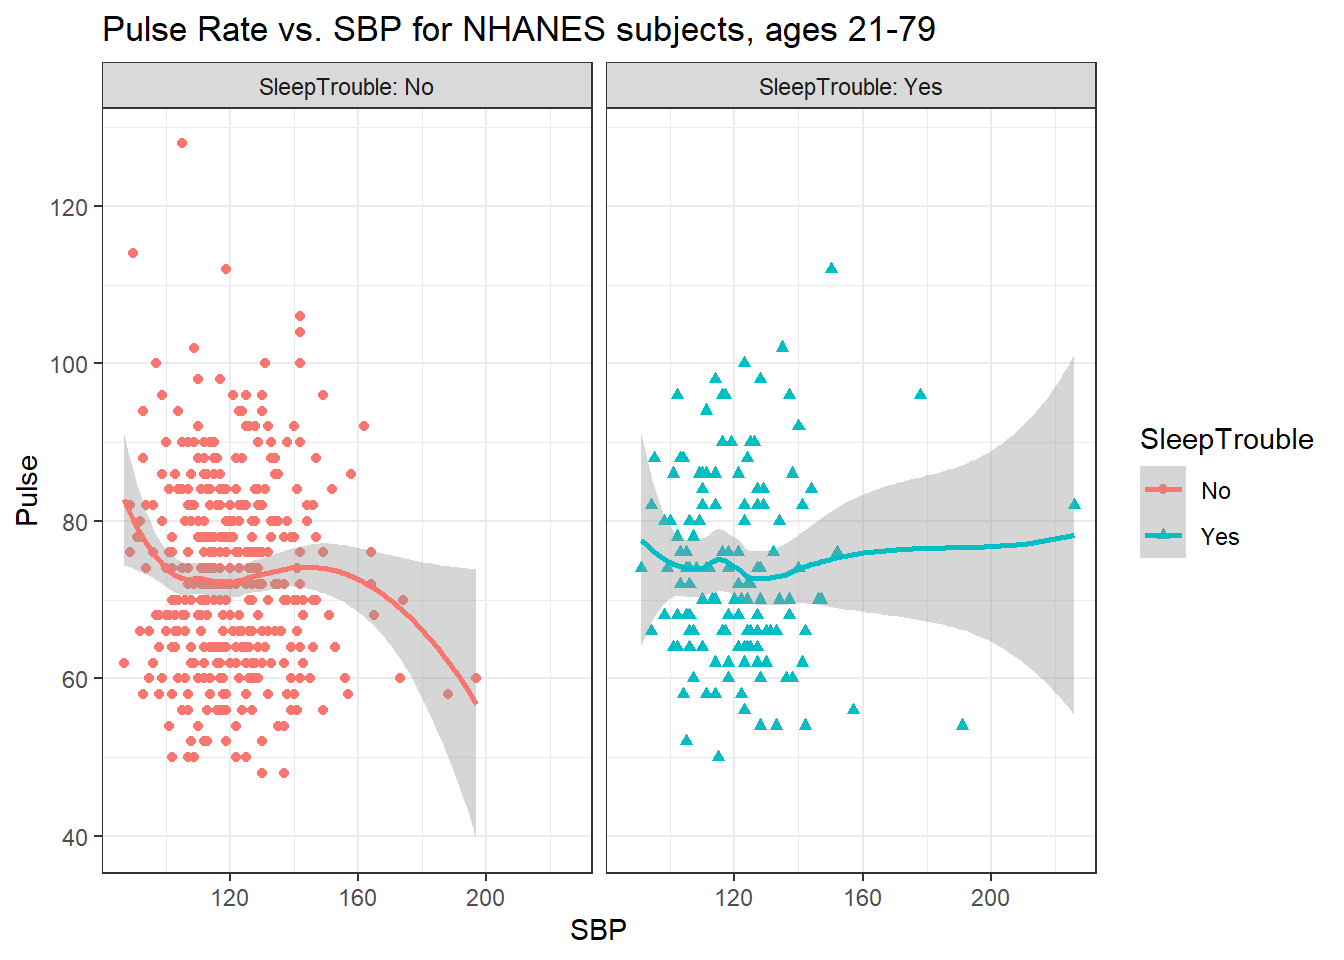
\includegraphics{431-notes_files/figure-latex/nh_dat3_sbpvspulsewithsleepfacets-fig-1.pdf}

\hypertarget{general-health-status}{%
\section{General Health Status}\label{general-health-status}}

Here's a Table of the General Health Status results. Again, this is a self-reported rating of each subject's health on a five point scale (Excellent, Very Good, Good, Fair, Poor.)

\begin{Shaded}
\begin{Highlighting}[]
\NormalTok{nh_dat3 }\OperatorTok
\StringTok{    }\KeywordTok{select}\NormalTok{(HealthGen) }\OperatorTok
\StringTok{    }\KeywordTok{table}\NormalTok{()}
\end{Highlighting}
\end{Shaded}

\begin{verbatim}
.
Excellent     Vgood      Good      Fair      Poor 
       64       196       238        83        22 
\end{verbatim}

The HealthGen data are categorical, which means that summarizing them with averages isn't as appealing as looking at percentages, proportions and rates.

Another, somewhat simpler way to get a table of this sort of information uses the \texttt{tabyl} function from the \texttt{janitor} package in R.

\begin{Shaded}
\begin{Highlighting}[]
\CommentTok{# tabyl is part of the janitor package}
\CommentTok{# already loaded: library(janitor)}

\NormalTok{nh_dat3 }\OperatorTok
\StringTok{    }\KeywordTok{tabyl}\NormalTok{(HealthGen) }
\end{Highlighting}
\end{Shaded}

\begin{verbatim}
 HealthGen   n    percent
 Excellent  64 0.10613599
     Vgood 196 0.32504146
      Good 238 0.39469320
      Fair  83 0.13764511
      Poor  22 0.03648425
\end{verbatim}

I don't actually like the title of \texttt{percent} here, as it's really a proportion, but that can be adjusted, and we can add a total.

\begin{Shaded}
\begin{Highlighting}[]
\NormalTok{nh_dat3 }\OperatorTok
\StringTok{    }\KeywordTok{tabyl}\NormalTok{(HealthGen) }\OperatorTok
\StringTok{    }\KeywordTok{adorn_totals}\NormalTok{() }\OperatorTok
\StringTok{    }\KeywordTok{adorn_pct_formatting}\NormalTok{()}
\end{Highlighting}
\end{Shaded}

\begin{verbatim}
 HealthGen   n percent
 Excellent  64   10.6%
     Vgood 196   32.5%
      Good 238   39.5%
      Fair  83   13.8%
      Poor  22    3.6%
     Total 603  100.0%
\end{verbatim}

When working with an unordered categorical variable, like \texttt{MaritalStatus}, the same approach can work.

\begin{Shaded}
\begin{Highlighting}[]
\NormalTok{nh_dat3 }\OperatorTok
\StringTok{    }\KeywordTok{tabyl}\NormalTok{(MaritalStatus) }\OperatorTok
\StringTok{    }\KeywordTok{adorn_totals}\NormalTok{() }\OperatorTok
\StringTok{    }\KeywordTok{adorn_pct_formatting}\NormalTok{()}
\end{Highlighting}
\end{Shaded}

\begin{verbatim}
 MaritalStatus   n percent
      Divorced  61   10.1%
   LivePartner  43    7.1%
       Married 349   57.9%
  NeverMarried 104   17.2%
     Separated   8    1.3%
       Widowed  38    6.3%
         Total 603  100.0%
\end{verbatim}

\hypertarget{bar-chart-for-categorical-data}{%
\subsection{Bar Chart for Categorical Data}\label{bar-chart-for-categorical-data}}

Usually, a \textbf{bar chart} is the best choice for a graphing a variable made up of categories.

\begin{Shaded}
\begin{Highlighting}[]
\KeywordTok{ggplot}\NormalTok{(}\DataTypeTok{data =}\NormalTok{ nh_dat3, }\KeywordTok{aes}\NormalTok{(}\DataTypeTok{x =}\NormalTok{ HealthGen)) }\OperatorTok{+}\StringTok{ }
\StringTok{    }\KeywordTok{geom_bar}\NormalTok{()}
\end{Highlighting}
\end{Shaded}

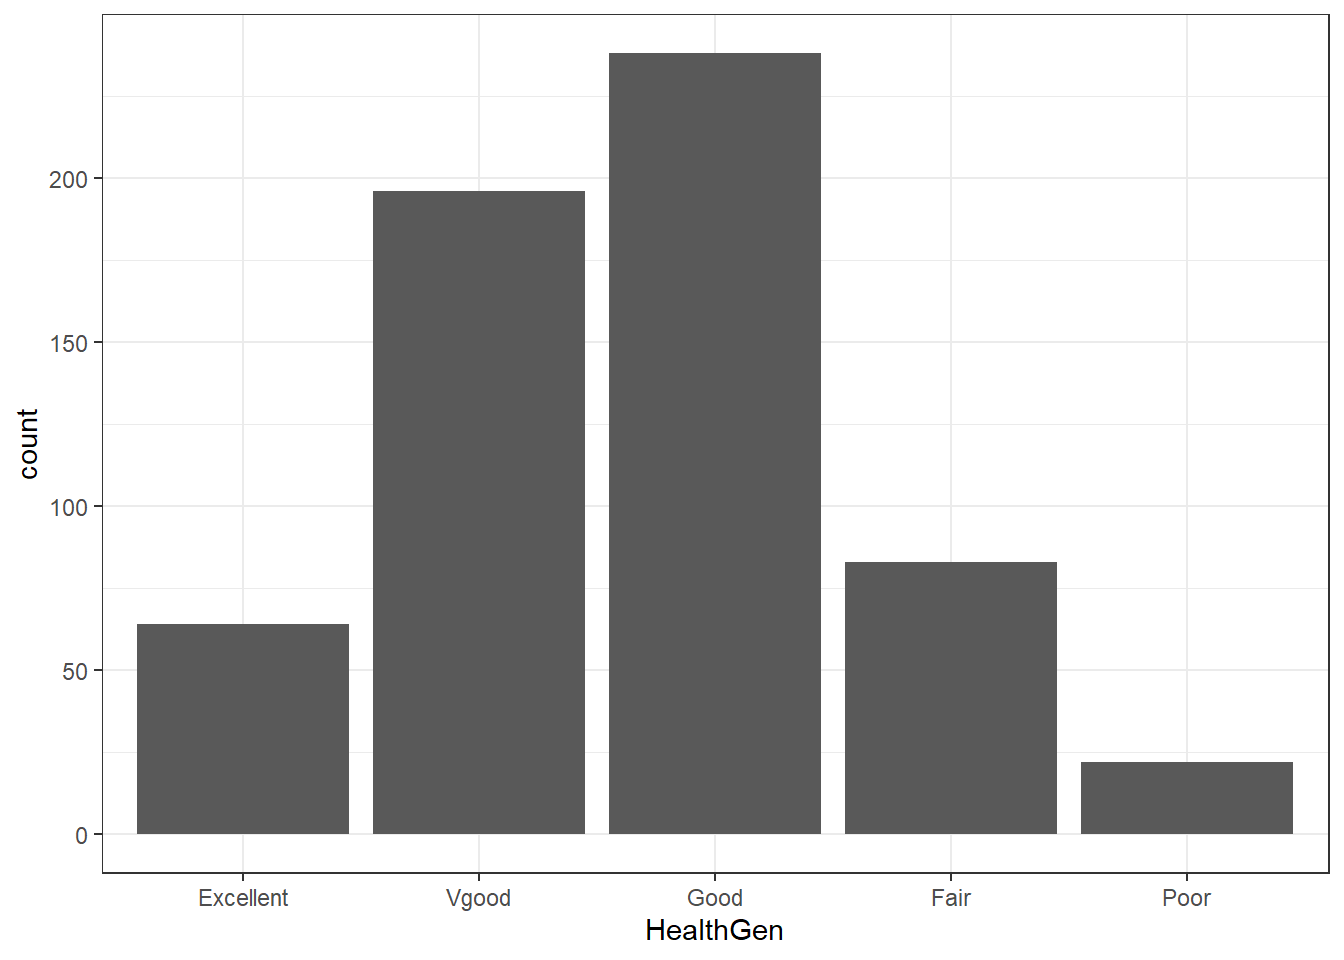
\includegraphics{431-notes_files/figure-latex/HealthGengraph1-fig-1.pdf}

There are lots of things we can do to make this plot fancier.

\begin{Shaded}
\begin{Highlighting}[]
\KeywordTok{ggplot}\NormalTok{(}\DataTypeTok{data =}\NormalTok{ nh_dat3, }\KeywordTok{aes}\NormalTok{(}\DataTypeTok{x =}\NormalTok{ HealthGen, }\DataTypeTok{fill =}\NormalTok{ HealthGen)) }\OperatorTok{+}\StringTok{ }
\StringTok{    }\KeywordTok{geom_bar}\NormalTok{() }\OperatorTok{+}\StringTok{ }
\StringTok{    }\KeywordTok{guides}\NormalTok{(}\DataTypeTok{fill =} \OtherTok{FALSE}\NormalTok{) }\OperatorTok{+}
\StringTok{    }\KeywordTok{labs}\NormalTok{(}\DataTypeTok{x =} \StringTok{"Self-Reported Health Status"}\NormalTok{,}
         \DataTypeTok{y =} \StringTok{"Number of NHANES subjects"}\NormalTok{,}
         \DataTypeTok{title =} \StringTok{"Self-Reported Health Status in NHANES subjects ages 21-79"}\NormalTok{)}
\end{Highlighting}
\end{Shaded}

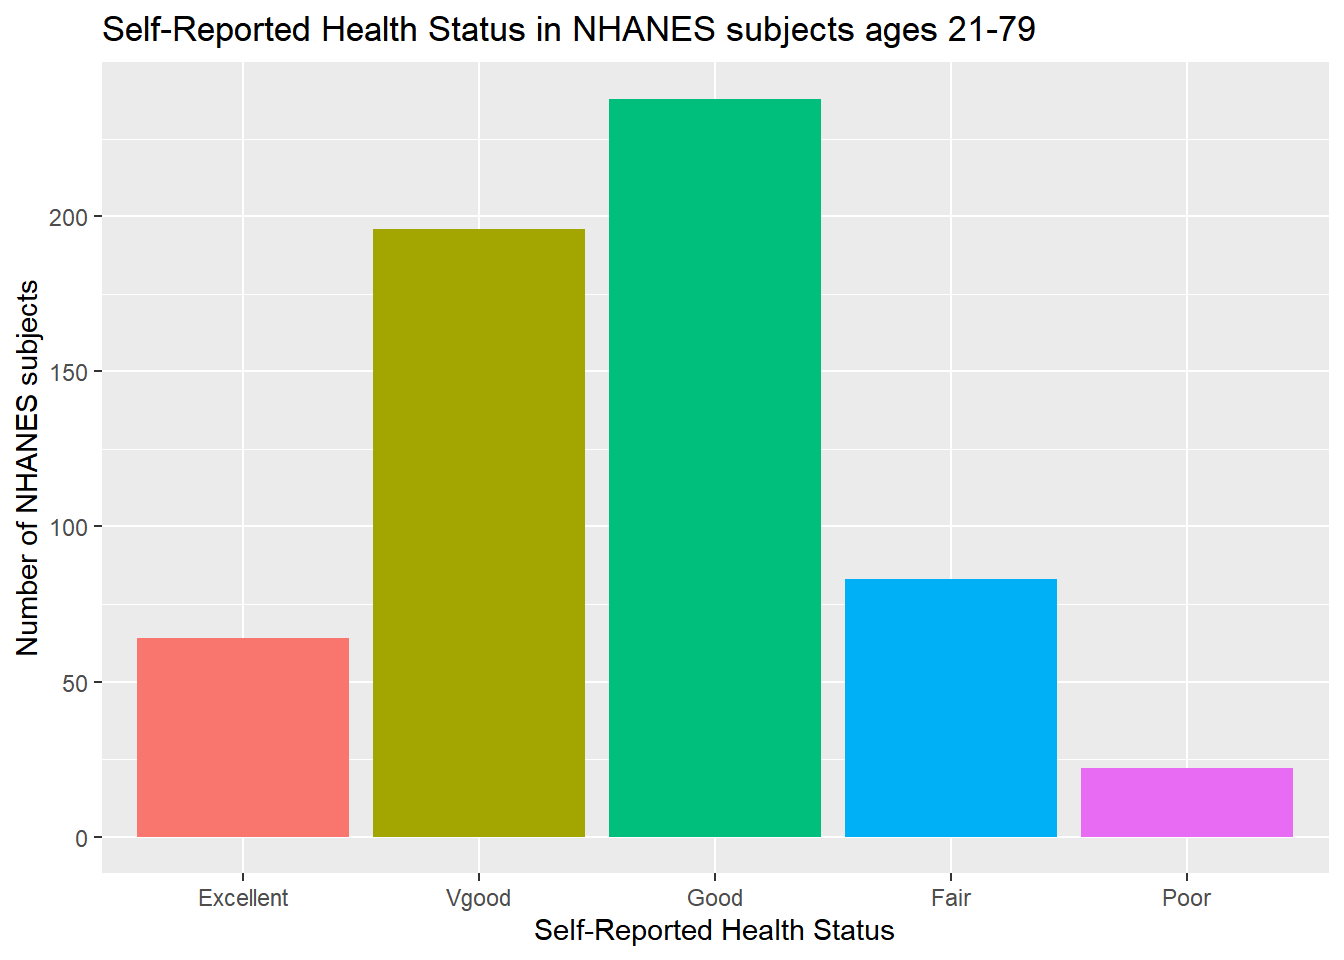
\includegraphics{431-notes_files/figure-latex/HealthGengraph2-fig-1.pdf}

Or, we can really go crazy\ldots{}

\begin{Shaded}
\begin{Highlighting}[]
\NormalTok{nh_dat3 }\OperatorTok
\StringTok{    }\KeywordTok{count}\NormalTok{(HealthGen) }\OperatorTok
\StringTok{    }\KeywordTok{ungroup}\NormalTok{() }\OperatorTok
\StringTok{    }\KeywordTok{mutate}\NormalTok{(}\DataTypeTok{pct =} \KeywordTok{round}\NormalTok{(}\KeywordTok{prop.table}\NormalTok{(n) }\OperatorTok{*}\StringTok{ }\DecValTok{100}\NormalTok{, }\DecValTok{1}\NormalTok{)) }\OperatorTok
\StringTok{    }\KeywordTok{ggplot}\NormalTok{(}\KeywordTok{aes}\NormalTok{(}\DataTypeTok{x =}\NormalTok{ HealthGen, }\DataTypeTok{y =}\NormalTok{ pct, }\DataTypeTok{fill =}\NormalTok{ HealthGen)) }\OperatorTok{+}\StringTok{ }
\StringTok{    }\KeywordTok{geom_bar}\NormalTok{(}\DataTypeTok{stat =} \StringTok{"identity"}\NormalTok{, }\DataTypeTok{position =} \StringTok{"dodge"}\NormalTok{) }\OperatorTok{+}
\StringTok{    }\KeywordTok{scale_fill_viridis_d}\NormalTok{() }\OperatorTok{+}
\StringTok{    }\KeywordTok{guides}\NormalTok{(}\DataTypeTok{fill =} \OtherTok{FALSE}\NormalTok{) }\OperatorTok{+}
\StringTok{    }\KeywordTok{geom_text}\NormalTok{(}\KeywordTok{aes}\NormalTok{(}\DataTypeTok{y =}\NormalTok{ pct }\OperatorTok{+}\StringTok{ }\DecValTok{1}\NormalTok{,    }\CommentTok{# nudge above top of bar}
                  \DataTypeTok{label =} \KeywordTok{paste0}\NormalTok{(pct, }\StringTok{'%'}\NormalTok{)),  }\CommentTok{# prettify}
              \DataTypeTok{position =} \KeywordTok{position_dodge}\NormalTok{(}\DataTypeTok{width =} \FloatTok{.9}\NormalTok{), }
              \DataTypeTok{size =} \DecValTok{4}\NormalTok{) }\OperatorTok{+}
\StringTok{    }\KeywordTok{labs}\NormalTok{(}\DataTypeTok{x =} \StringTok{"Self-Reported Health Status"}\NormalTok{,}
         \DataTypeTok{y =} \StringTok{"Percentage of NHANES subjects"}\NormalTok{,}
         \DataTypeTok{title =} \StringTok{"Self-Reported Health Status in NHANES subjects ages 21-79"}\NormalTok{) }\OperatorTok{+}
\StringTok{    }\KeywordTok{theme_bw}\NormalTok{()}
\end{Highlighting}
\end{Shaded}

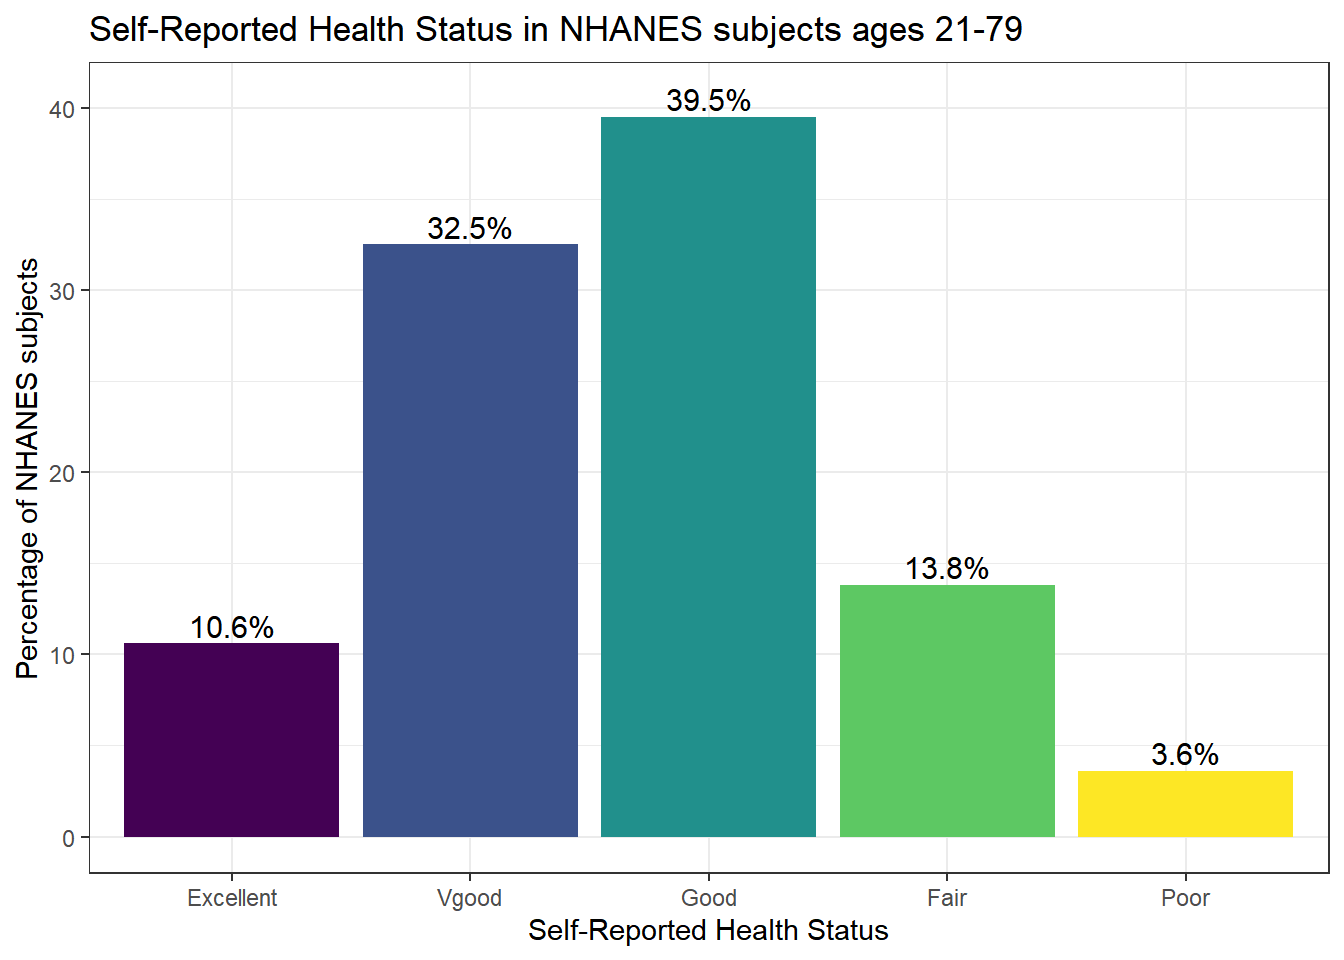
\includegraphics{431-notes_files/figure-latex/HealthGengraph3-fig-1.pdf}

\hypertarget{working-with-tables}{%
\subsection{Working with Tables}\label{working-with-tables}}

We can add both row and column marginal totals, and compare subjects by Sex, as follows\ldots{}

\begin{Shaded}
\begin{Highlighting}[]
\NormalTok{nh_dat3 }\OperatorTok
\StringTok{    }\KeywordTok{tabyl}\NormalTok{(Sex, HealthGen) }\OperatorTok
\StringTok{    }\KeywordTok{adorn_totals}\NormalTok{(}\KeywordTok{c}\NormalTok{(}\StringTok{"row"}\NormalTok{, }\StringTok{"col"}\NormalTok{)) }
\end{Highlighting}
\end{Shaded}

\begin{verbatim}
    Sex Excellent Vgood Good Fair Poor Total
 female        27    96  121   41   14   299
   male        37   100  117   42    8   304
  Total        64   196  238   83   22   603
\end{verbatim}

If we like, we can make this look a little more polished with the \texttt{knitr::kable} function\ldots{}

\begin{Shaded}
\begin{Highlighting}[]
\NormalTok{nh_dat3 }\OperatorTok
\StringTok{    }\KeywordTok{tabyl}\NormalTok{(Sex, HealthGen) }\OperatorTok
\StringTok{    }\KeywordTok{adorn_totals}\NormalTok{(}\KeywordTok{c}\NormalTok{(}\StringTok{"row"}\NormalTok{, }\StringTok{"col"}\NormalTok{)) }\OperatorTok
\StringTok{    }\NormalTok{knitr}\OperatorTok{::}\KeywordTok{kable}\NormalTok{()}
\end{Highlighting}
\end{Shaded}

\begin{tabular}{l|r|r|r|r|r|r}
\hline
Sex & Excellent & Vgood & Good & Fair & Poor & Total\\
\hline
female & 27 & 96 & 121 & 41 & 14 & 299\\
\hline
male & 37 & 100 & 117 & 42 & 8 & 304\\
\hline
Total & 64 & 196 & 238 & 83 & 22 & 603\\
\hline
\end{tabular}

Or, we can get a complete cross-tabulation, including (in this case) the percentages of people within each Sex that fall in each HealthGen category (percentages within each row) like this.

\begin{Shaded}
\begin{Highlighting}[]
\NormalTok{nh_dat3 }\OperatorTok
\StringTok{    }\KeywordTok{tabyl}\NormalTok{(Sex, HealthGen) }\OperatorTok
\StringTok{    }\KeywordTok{adorn_totals}\NormalTok{(}\StringTok{"row"}\NormalTok{) }\OperatorTok
\StringTok{    }\KeywordTok{adorn_percentages}\NormalTok{(}\StringTok{"row"}\NormalTok{) }\OperatorTok
\StringTok{    }\KeywordTok{adorn_pct_formatting}\NormalTok{() }\OperatorTok
\StringTok{    }\KeywordTok{adorn_ns}\NormalTok{() }\OperatorTok
\StringTok{    }\NormalTok{knitr}\OperatorTok{::}\KeywordTok{kable}\NormalTok{()}
\end{Highlighting}
\end{Shaded}

\begin{tabular}{l|l|l|l|l|l}
\hline
Sex & Excellent & Vgood & Good & Fair & Poor\\
\hline
female & 9.0\% (27) & 32.1\%  (96) & 40.5\% (121) & 13.7\% (41) & 4.7\% (14)\\
\hline
male & 12.2\% (37) & 32.9\% (100) & 38.5\% (117) & 13.8\% (42) & 2.6\%  (8)\\
\hline
Total & 10.6\% (64) & 32.5\% (196) & 39.5\% (238) & 13.8\% (83) & 3.6\% (22)\\
\hline
\end{tabular}

And, if we wanted the column percentages, to determine which sex had the higher rate of each HealthGen status level, we can get that by changing the adorn\_percentages to describe results at the column level:

\begin{Shaded}
\begin{Highlighting}[]
\NormalTok{nh_dat3 }\OperatorTok
\StringTok{    }\KeywordTok{tabyl}\NormalTok{(Sex, HealthGen) }\OperatorTok
\StringTok{    }\KeywordTok{adorn_totals}\NormalTok{(}\StringTok{"col"}\NormalTok{) }\OperatorTok
\StringTok{    }\KeywordTok{adorn_percentages}\NormalTok{(}\StringTok{"col"}\NormalTok{) }\OperatorTok
\StringTok{    }\KeywordTok{adorn_pct_formatting}\NormalTok{() }\OperatorTok
\StringTok{    }\KeywordTok{adorn_ns}\NormalTok{() }\OperatorTok
\StringTok{    }\NormalTok{knitr}\OperatorTok{::}\KeywordTok{kable}\NormalTok{()}
\end{Highlighting}
\end{Shaded}

\begin{tabular}{l|l|l|l|l|l|l}
\hline
Sex & Excellent & Vgood & Good & Fair & Poor & Total\\
\hline
female & 42.2\% (27) & 49.0\%  (96) & 50.8\% (121) & 49.4\% (41) & 63.6\% (14) & 49.6\% (299)\\
\hline
male & 57.8\% (37) & 51.0\% (100) & 49.2\% (117) & 50.6\% (42) & 36.4\%  (8) & 50.4\% (304)\\
\hline
\end{tabular}

\hypertarget{sbp-by-general-health-status}{%
\subsection{SBP by General Health Status}\label{sbp-by-general-health-status}}

Let's consider now the relationship between self-reported overall health and systolic blood pressure.

\begin{Shaded}
\begin{Highlighting}[]
\KeywordTok{ggplot}\NormalTok{(}\DataTypeTok{data =}\NormalTok{ nh_dat3, }\KeywordTok{aes}\NormalTok{(}\DataTypeTok{x =}\NormalTok{ HealthGen, }\DataTypeTok{y =}\NormalTok{ SBP, }\DataTypeTok{fill =}\NormalTok{ HealthGen)) }\OperatorTok{+}\StringTok{ }
\StringTok{    }\KeywordTok{geom_boxplot}\NormalTok{() }\OperatorTok{+}\StringTok{ }
\StringTok{    }\KeywordTok{labs}\NormalTok{(}\DataTypeTok{title =} \StringTok{"SBP by Health Status, Overall Health for NHANES ages 21-79"}\NormalTok{,}
         \DataTypeTok{y =} \StringTok{"Systolic Blood Pressure"}\NormalTok{, }\DataTypeTok{x =} \StringTok{"Self-Reported Overall Health"}\NormalTok{) }\OperatorTok{+}\StringTok{ }
\StringTok{    }\KeywordTok{guides}\NormalTok{(}\DataTypeTok{fill =} \OtherTok{FALSE}\NormalTok{) }
\end{Highlighting}
\end{Shaded}

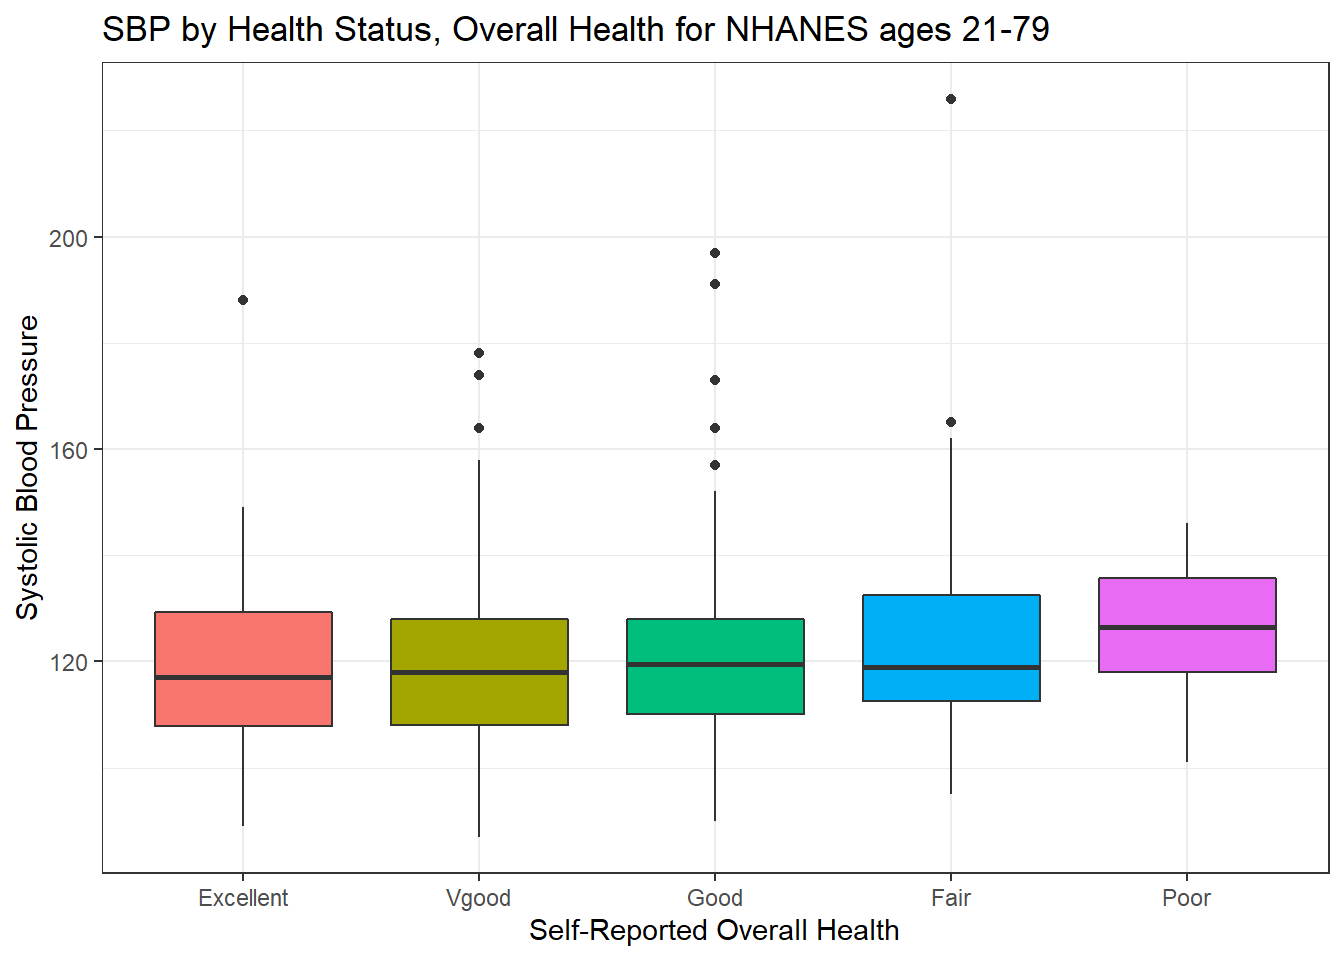
\includegraphics{431-notes_files/figure-latex/nh_dat3_sbpbyhealth-fig-1.pdf}

We can see that not too many people self-identify with the ``Poor'' health category.

\begin{Shaded}
\begin{Highlighting}[]
\NormalTok{nh_dat3 }\OperatorTok
\StringTok{    }\KeywordTok{group_by}\NormalTok{(HealthGen) }\OperatorTok
\StringTok{    }\KeywordTok{summarise}\NormalTok{(}\DataTypeTok{count =} \KeywordTok{n}\NormalTok{(), }\KeywordTok{mean}\NormalTok{(SBP), }\KeywordTok{median}\NormalTok{(SBP)) }\OperatorTok
\StringTok{    }\NormalTok{knitr}\OperatorTok{::}\KeywordTok{kable}\NormalTok{() }
\end{Highlighting}
\end{Shaded}

\begin{verbatim}
`summarise()` ungrouping output (override with `.groups` argument)
\end{verbatim}

\begin{tabular}{l|r|r|r}
\hline
HealthGen & count & mean(SBP) & median(SBP)\\
\hline
Excellent & 64 & 119.1562 & 117.0\\
\hline
Vgood & 196 & 119.0714 & 118.0\\
\hline
Good & 238 & 120.4244 & 119.5\\
\hline
Fair & 83 & 123.9398 & 119.0\\
\hline
Poor & 22 & 125.8636 & 126.5\\
\hline
\end{tabular}

\hypertarget{sbp-by-physical-activity-and-general-health-status}{%
\subsection{SBP by Physical Activity and General Health Status}\label{sbp-by-physical-activity-and-general-health-status}}

We'll build a panel of boxplots to try to understand the relationships between Systolic Blood Pressure, General Health Status and Physical Activity. Note the use of \texttt{coord\_flip} to rotate the graph 90 degrees, and the use of \texttt{labeller} within \texttt{facet\_wrap} to include both the name of the (Physical Activity) variable and its value.

\begin{Shaded}
\begin{Highlighting}[]
\KeywordTok{ggplot}\NormalTok{(}\DataTypeTok{data =}\NormalTok{ nh_dat3, }\KeywordTok{aes}\NormalTok{(}\DataTypeTok{x =}\NormalTok{ HealthGen, }\DataTypeTok{y =}\NormalTok{ SBP, }\DataTypeTok{fill =}\NormalTok{ HealthGen)) }\OperatorTok{+}\StringTok{ }
\StringTok{    }\KeywordTok{geom_boxplot}\NormalTok{() }\OperatorTok{+}\StringTok{ }
\StringTok{    }\KeywordTok{labs}\NormalTok{(}\DataTypeTok{title =} \StringTok{"SBP by Health Status, Overall Health for NHANES ages 21-79"}\NormalTok{,}
         \DataTypeTok{y =} \StringTok{"Body-mass index"}\NormalTok{, }\DataTypeTok{x =} \StringTok{"Self-Reported Overall Health"}\NormalTok{) }\OperatorTok{+}\StringTok{ }
\StringTok{    }\KeywordTok{guides}\NormalTok{(}\DataTypeTok{fill =} \OtherTok{FALSE}\NormalTok{) }\OperatorTok{+}
\StringTok{    }\KeywordTok{facet_wrap}\NormalTok{(}\OperatorTok{~}\StringTok{ }\NormalTok{PhysActive, }\DataTypeTok{labeller =} \StringTok{"label_both"}\NormalTok{) }\OperatorTok{+}\StringTok{ }
\StringTok{    }\KeywordTok{coord_flip}\NormalTok{()}
\end{Highlighting}
\end{Shaded}

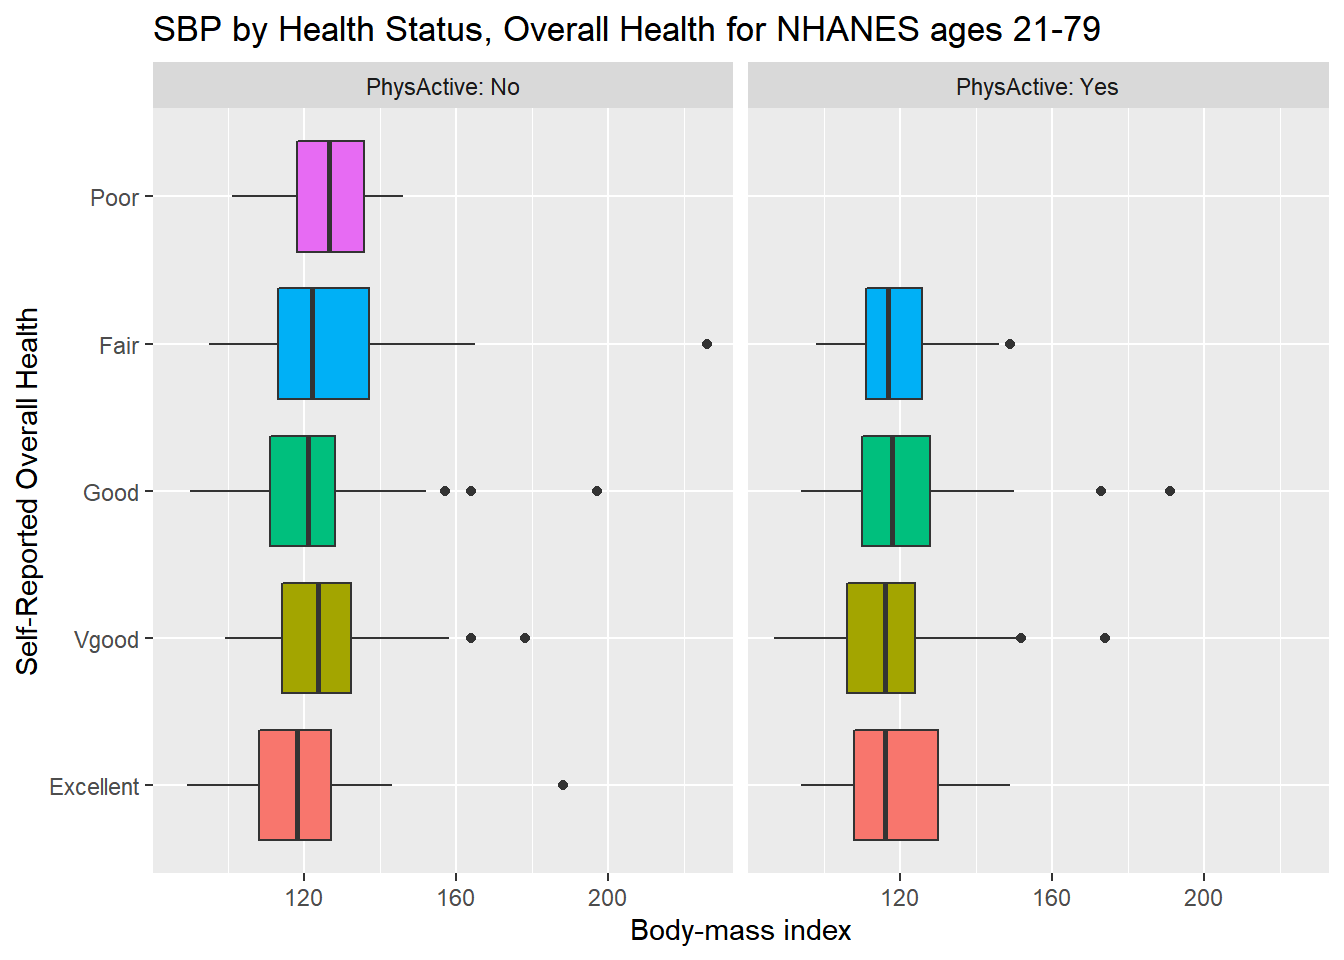
\includegraphics{431-notes_files/figure-latex/nh_dat3_bmibyhealthbysex1-fig-1.pdf}

\hypertarget{sbp-by-sleep-trouble-and-general-health-status}{%
\subsection{SBP by Sleep Trouble and General Health Status}\label{sbp-by-sleep-trouble-and-general-health-status}}

Here's a plot of faceted histograms, which might be used to address similar questions related to the relationship between Overall Health, Systolic Blood Pressure and Sex.

\begin{Shaded}
\begin{Highlighting}[]
\KeywordTok{ggplot}\NormalTok{(}\DataTypeTok{data =}\NormalTok{ nh_dat3, }\KeywordTok{aes}\NormalTok{(}\DataTypeTok{x =}\NormalTok{ SBP, }\DataTypeTok{fill =}\NormalTok{ Sex)) }\OperatorTok{+}\StringTok{ }
\StringTok{    }\KeywordTok{geom_histogram}\NormalTok{(}\DataTypeTok{color =} \StringTok{"white"}\NormalTok{, }\DataTypeTok{bins =} \DecValTok{20}\NormalTok{) }\OperatorTok{+}\StringTok{ }
\StringTok{    }\KeywordTok{labs}\NormalTok{(}\DataTypeTok{title =} \StringTok{"SBP by Sex, Overall Health for NHANES ages 21-79"}\NormalTok{,}
         \DataTypeTok{x =} \StringTok{"Body-mass index"}\NormalTok{) }\OperatorTok{+}\StringTok{ }
\StringTok{    }\KeywordTok{guides}\NormalTok{(}\DataTypeTok{fill =} \OtherTok{FALSE}\NormalTok{) }\OperatorTok{+}
\StringTok{    }\KeywordTok{facet_grid}\NormalTok{(HealthGen }\OperatorTok{~}\StringTok{ }\NormalTok{Sex)}
\end{Highlighting}
\end{Shaded}

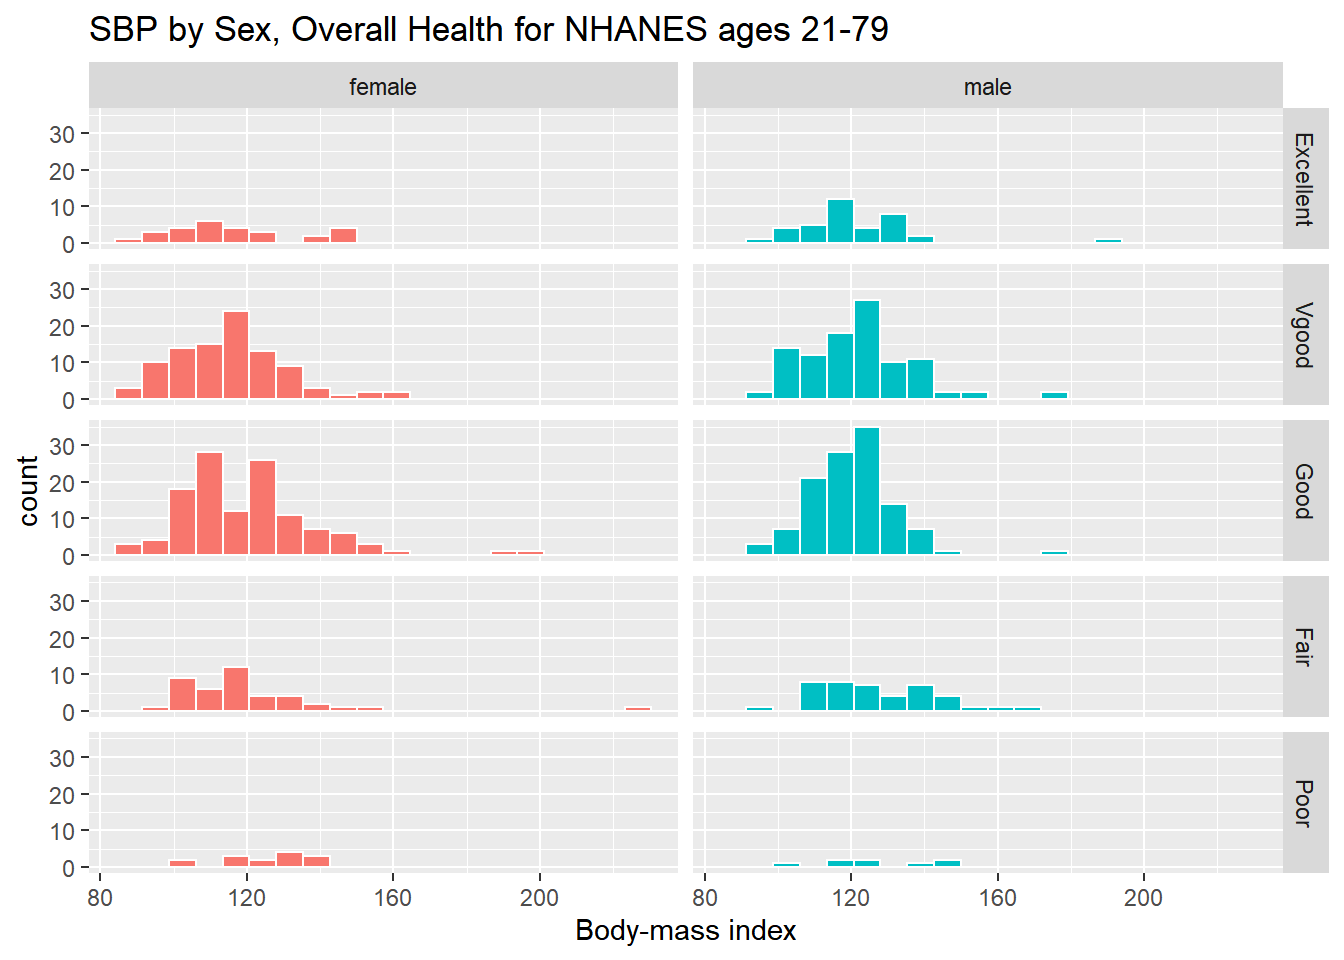
\includegraphics{431-notes_files/figure-latex/nh_dat3_bmibyhealthbysex2-fig-1.pdf}

\hypertarget{conclusions}{%
\section{Conclusions}\label{conclusions}}

This is just a small piece of the toolbox for visualizations that we'll create in this class. Many additional tools are on the way, but the main idea won't change. Using the \texttt{ggplot2} package, we can accomplish several critical tasks in creating a visualization, including:

\begin{itemize}
\tightlist
\item
  Identifying (and labeling) the axes and titles
\item
  Identifying a type of \texttt{geom} to use, like a point, bar or histogram
\item
  Changing fill, color, shape, size to facilitate comparisons
\item
  Building ``small multiples'' of plots with faceting
\end{itemize}

Good data visualizations make it easy to see the data, and \texttt{ggplot2}'s tools make it relatively difficult to make a really bad graph.

\hypertarget{data-structures-and-types-of-variables}{%
\chapter{Data Structures and Types of Variables}\label{data-structures-and-types-of-variables}}

\hypertarget{data-require-structure-and-context}{%
\section{Data require structure and context}\label{data-require-structure-and-context}}

\textbf{Descriptive statistics} are concerned with the presentation, organization and summary of data, as suggested in \citet{Norman-Streiner}. This includes various methods of organizing and graphing data to get an idea of what those data can tell us.

As \citet{Vittinghoff} suggest, the nature of the measurement determines how best to describe it statistically, and the main distinction is between \textbf{numerical} and \textbf{categorical} variables. Even this is a little tricky - plenty of data can have values that look like numerical values, but are just numerals serving as labels.

As \citet{BockVD} point out, the truly critical notion, of course, is that data values, no matter what kind, are useless without their contexts. The Five W's (Who, What {[}and in what units{]}, When, Where, Why, and often How) are just as useful for establishing the context of data as they are in journalism. If you can't answer Who and What, in particular, you don't have any useful information.

In general, each row of a data frame corresponds to an individual (respondent, experimental unit, record, or observation) about whom some characteristics are gathered in columns (and these characteristics may be called variables, factors or data elements.) Every column / variable should have a name that indicates \emph{what} it is measuring, and every row / observation should have a name that indicates \emph{who} is being measured.

\hypertarget{newNHANES}{%
\section{A New NHANES Adult Sample}\label{newNHANES}}

In Chapter \ref{dataviz}, we spent some time with a sample from the National Health and Nutrition Examination. Now, by changing the value of the \texttt{set.seed} function which determines the starting place for the random sampling, and changing some other specifications, we'll generate a new sample describing 500 adult subjects who completed the 2011-12 version of the survey when they were between the ages of 21 and 64.

Note also that what is listed in the NHANES data frame as \texttt{Gender} should be more correctly referred to as \texttt{sex}. \texttt{Sex} is a biological feature of an individual, while \texttt{Gender} is a social construct. This is an important distinction, so I'll change the name of the variable. I'm also changing the names of three other variables, to create \texttt{Race}, \texttt{SBP} and \texttt{DBP}.

\begin{Shaded}
\begin{Highlighting}[]
\CommentTok{# library(NHANES) # NHANES package/library of functions, data}

\NormalTok{nh_temp <-}\StringTok{ }\NormalTok{NHANES }\OperatorTok
\StringTok{    }\KeywordTok{filter}\NormalTok{(SurveyYr }\OperatorTok{==}\StringTok{ "2011_12"}\NormalTok{) }\OperatorTok
\StringTok{    }\KeywordTok{filter}\NormalTok{(Age }\OperatorTok{>=}\StringTok{ }\DecValTok{21} \OperatorTok{&}\StringTok{ }\NormalTok{Age }\OperatorTok{<}\StringTok{ }\DecValTok{65}\NormalTok{) }\OperatorTok
\StringTok{    }\KeywordTok{mutate}\NormalTok{(}\DataTypeTok{Sex =}\NormalTok{ Gender, }\DataTypeTok{Race =}\NormalTok{ Race3, }\DataTypeTok{SBP =}\NormalTok{ BPSysAve, }\DataTypeTok{DBP =}\NormalTok{ BPDiaAve) }\OperatorTok
\StringTok{    }\KeywordTok{select}\NormalTok{(ID, Sex, Age, Race, Education, BMI, SBP, DBP, }
\NormalTok{           Pulse, PhysActive, Smoke100, SleepTrouble, }
\NormalTok{           MaritalStatus, HealthGen)}

\KeywordTok{set.seed}\NormalTok{(}\DecValTok{431002}\NormalTok{) }
\CommentTok{# use set.seed to ensure that we all get the same random sample }

\NormalTok{nh_adults <-}\StringTok{ }\KeywordTok{sample_n}\NormalTok{(nh_temp, }\DataTypeTok{size =} \DecValTok{500}\NormalTok{) }

\NormalTok{nh_adults}
\end{Highlighting}
\end{Shaded}

\begin{verbatim}
# A tibble: 500 x 14
      ID Sex     Age Race  Education   BMI   SBP   DBP Pulse PhysActive Smoke100
   <int> <fct> <int> <fct> <fct>     <dbl> <int> <int> <int> <fct>      <fct>   
 1 71531 male     35 White Some Col~  22.4   143    90    84 Yes        No      
 2 68613 fema~    61 White Some Col~  27.7   119    86   112 No         No      
 3 67064 male     31 White College ~  26.6   110    76    86 Yes        Yes     
 4 63924 fema~    29 Black High Sch~  41.9    98    56    74 No         Yes     
 5 62840 male     60 White 8th Grade  35.8   127     0   110 No         Yes     
 6 68058 male     50 White Some Col~  30.6    NA    NA    NA No         Yes     
 7 68936 fema~    36 Black High Sch~  30.5   119    69    60 No         No      
 8 71189 male     51 White College ~  25.6   112    70    54 Yes        Yes     
 9 69936 fema~    54 Asian College ~  21.8   126    80    78 Yes        No      
10 70687 male     59 White College ~  25.5   149    89    62 Yes        No      
# ... with 490 more rows, and 3 more variables: SleepTrouble <fct>,
#   MaritalStatus <fct>, HealthGen <fct>
\end{verbatim}

The data consist of 500 rows (observations) on 13 variables (columns). Essentially, we have 13 pieces of information on each of 500 adult NHANES subjects who were included in the 2011-12 panel.

\hypertarget{summarizing-the-datas-structure}{%
\subsection{Summarizing the Data's Structure}\label{summarizing-the-datas-structure}}

We can identify the number of rows and columns in a data frame or tibble with the \texttt{dim} function.

\begin{Shaded}
\begin{Highlighting}[]
\KeywordTok{dim}\NormalTok{(nh_adults)}
\end{Highlighting}
\end{Shaded}

\begin{verbatim}
[1] 500  14
\end{verbatim}

The \texttt{str} function provides a lot of information about the structure of a data frame or tibble.

\begin{Shaded}
\begin{Highlighting}[]
\KeywordTok{str}\NormalTok{(nh_adults)}
\end{Highlighting}
\end{Shaded}

\begin{verbatim}
tibble [500 x 14] (S3: tbl_df/tbl/data.frame)
 $ ID           : int [1:500] 71531 68613 67064 63924 62840 68058 68936 71189 69936 70687 ...
 $ Sex          : Factor w/ 2 levels "female","male": 2 1 2 1 2 2 1 2 1 2 ...
 $ Age          : int [1:500] 35 61 31 29 60 50 36 51 54 59 ...
 $ Race         : Factor w/ 6 levels "Asian","Black",..: 5 5 5 2 5 5 2 5 1 5 ...
 $ Education    : Factor w/ 5 levels "8th Grade","9 - 11th Grade",..: 4 4 5 3 1 4 3 5 5 5 ...
 $ BMI          : num [1:500] 22.4 27.7 26.6 41.9 35.8 30.6 30.5 25.6 21.8 25.5 ...
 $ SBP          : int [1:500] 143 119 110 98 127 NA 119 112 126 149 ...
 $ DBP          : int [1:500] 90 86 76 56 0 NA 69 70 80 89 ...
 $ Pulse        : int [1:500] 84 112 86 74 110 NA 60 54 78 62 ...
 $ PhysActive   : Factor w/ 2 levels "No","Yes": 2 1 2 1 1 1 1 2 2 2 ...
 $ Smoke100     : Factor w/ 2 levels "No","Yes": 1 1 2 2 2 2 1 2 1 1 ...
 $ SleepTrouble : Factor w/ 2 levels "No","Yes": 2 1 1 2 2 2 1 1 1 1 ...
 $ MaritalStatus: Factor w/ 6 levels "Divorced","LivePartner",..: 4 6 3 5 3 3 4 3 3 6 ...
 $ HealthGen    : Factor w/ 5 levels "Excellent","Vgood",..: 3 2 3 4 5 3 3 NA 3 1 ...
\end{verbatim}

To see the first few observations, use \texttt{head}, and to see the last few, try \texttt{tail}\ldots{}

\begin{Shaded}
\begin{Highlighting}[]
\KeywordTok{tail}\NormalTok{(nh_adults, }\DecValTok{5}\NormalTok{) }\CommentTok{# shows the last five observations in the data set}
\end{Highlighting}
\end{Shaded}

\begin{verbatim}
# A tibble: 5 x 14
     ID Sex     Age Race  Education   BMI   SBP   DBP Pulse PhysActive Smoke100
  <int> <fct> <int> <fct> <fct>     <dbl> <int> <int> <int> <fct>      <fct>   
1 66770 fema~    22 White Some Col~  44.6   100    90    92 Yes        No      
2 68754 male     57 White Some Col~  23.2   124    85    82 No         Yes     
3 70911 male     59 White College ~  24.5   118    57    76 No         Yes     
4 71393 male     27 White High Sch~  25.7   116    61    88 Yes        No      
5 70458 fema~    35 Black 9 - 11th~  21.9   115    64    84 No         No      
# ... with 3 more variables: SleepTrouble <fct>, MaritalStatus <fct>,
#   HealthGen <fct>
\end{verbatim}

\hypertarget{what-are-the-variables}{%
\subsection{What are the variables?}\label{what-are-the-variables}}

We can use the \texttt{glimpse} function to get a short preview of the data.

\begin{Shaded}
\begin{Highlighting}[]
\KeywordTok{glimpse}\NormalTok{(nh_adults)}
\end{Highlighting}
\end{Shaded}

\begin{verbatim}
Rows: 500
Columns: 14
$ ID            <int> 71531, 68613, 67064, 63924, 62840, 68058, 68936, 7118...
$ Sex           <fct> male, female, male, female, male, male, female, male,...
$ Age           <int> 35, 61, 31, 29, 60, 50, 36, 51, 54, 59, 59, 27, 44, 4...
$ Race          <fct> White, White, White, Black, White, White, Black, Whit...
$ Education     <fct> Some College, Some College, College Grad, High School...
$ BMI           <dbl> 22.4, 27.7, 26.6, 41.9, 35.8, 30.6, 30.5, 25.6, 21.8,...
$ SBP           <int> 143, 119, 110, 98, 127, NA, 119, 112, 126, 149, 122, ...
$ DBP           <int> 90, 86, 76, 56, 0, NA, 69, 70, 80, 89, 75, 78, 69, 78...
$ Pulse         <int> 84, 112, 86, 74, 110, NA, 60, 54, 78, 62, 82, 68, 76,...
$ PhysActive    <fct> Yes, No, Yes, No, No, No, No, Yes, Yes, Yes, No, Yes,...
$ Smoke100      <fct> No, No, Yes, Yes, Yes, Yes, No, Yes, No, No, No, No, ...
$ SleepTrouble  <fct> Yes, No, No, Yes, Yes, Yes, No, No, No, No, No, No, N...
$ MaritalStatus <fct> NeverMarried, Widowed, Married, Separated, Married, M...
$ HealthGen     <fct> Good, Vgood, Good, Fair, Poor, Good, Good, NA, Good, ...
\end{verbatim}

The variables we have collected are described in the brief table below\footnote{Descriptions are adapted from the ?NHANES help file. Remember that what NHANES lists as Gender is captured here as Sex, and similarly Race3, BPSysAve and BPDiaAve from NHANES are here listed as Race, SBP and DBP.}.

\begin{longtable}[]{@{}rll@{}}
\toprule
\begin{minipage}[b]{0.15\columnwidth}\raggedleft
Variable\strut
\end{minipage} & \begin{minipage}[b]{0.58\columnwidth}\raggedright
Description\strut
\end{minipage} & \begin{minipage}[b]{0.18\columnwidth}\raggedright
Sample Values\strut
\end{minipage}\tabularnewline
\midrule
\endhead
\begin{minipage}[t]{0.15\columnwidth}\raggedleft
ID\strut
\end{minipage} & \begin{minipage}[t]{0.58\columnwidth}\raggedright
a numerical code identifying the subject\strut
\end{minipage} & \begin{minipage}[t]{0.18\columnwidth}\raggedright
64427, 63788\strut
\end{minipage}\tabularnewline
\begin{minipage}[t]{0.15\columnwidth}\raggedleft
Sex\strut
\end{minipage} & \begin{minipage}[t]{0.58\columnwidth}\raggedright
sex of subject (2 levels)\strut
\end{minipage} & \begin{minipage}[t]{0.18\columnwidth}\raggedright
male, female\strut
\end{minipage}\tabularnewline
\begin{minipage}[t]{0.15\columnwidth}\raggedleft
Age\strut
\end{minipage} & \begin{minipage}[t]{0.58\columnwidth}\raggedright
age (years) at screening of subject\strut
\end{minipage} & \begin{minipage}[t]{0.18\columnwidth}\raggedright
37, 40\strut
\end{minipage}\tabularnewline
\begin{minipage}[t]{0.15\columnwidth}\raggedleft
Race\strut
\end{minipage} & \begin{minipage}[t]{0.58\columnwidth}\raggedright
reported race of subject (6 levels)\strut
\end{minipage} & \begin{minipage}[t]{0.18\columnwidth}\raggedright
White, Asian\strut
\end{minipage}\tabularnewline
\begin{minipage}[t]{0.15\columnwidth}\raggedleft
Education\strut
\end{minipage} & \begin{minipage}[t]{0.58\columnwidth}\raggedright
educational level of subject (5 levels)\strut
\end{minipage} & \begin{minipage}[t]{0.18\columnwidth}\raggedright
College Grad, High School\strut
\end{minipage}\tabularnewline
\begin{minipage}[t]{0.15\columnwidth}\raggedleft
BMI\strut
\end{minipage} & \begin{minipage}[t]{0.58\columnwidth}\raggedright
body-mass index, in kg/m\textsuperscript{2}\strut
\end{minipage} & \begin{minipage}[t]{0.18\columnwidth}\raggedright
36.5, 18.2\strut
\end{minipage}\tabularnewline
\begin{minipage}[t]{0.15\columnwidth}\raggedleft
SBP\strut
\end{minipage} & \begin{minipage}[t]{0.58\columnwidth}\raggedright
systolic blood pressure in mm Hg\strut
\end{minipage} & \begin{minipage}[t]{0.18\columnwidth}\raggedright
111, 115\strut
\end{minipage}\tabularnewline
\begin{minipage}[t]{0.15\columnwidth}\raggedleft
DBP\strut
\end{minipage} & \begin{minipage}[t]{0.58\columnwidth}\raggedright
diastolic blood pressure in mm Hg\strut
\end{minipage} & \begin{minipage}[t]{0.18\columnwidth}\raggedright
72, 74\strut
\end{minipage}\tabularnewline
\begin{minipage}[t]{0.15\columnwidth}\raggedleft
Pulse\strut
\end{minipage} & \begin{minipage}[t]{0.58\columnwidth}\raggedright
60 second pulse rate in beats per minute\strut
\end{minipage} & \begin{minipage}[t]{0.18\columnwidth}\raggedright
56, 102\strut
\end{minipage}\tabularnewline
\begin{minipage}[t]{0.15\columnwidth}\raggedleft
PhysActive\strut
\end{minipage} & \begin{minipage}[t]{0.58\columnwidth}\raggedright
Moderate or vigorous-intensity sports?\strut
\end{minipage} & \begin{minipage}[t]{0.18\columnwidth}\raggedright
Yes, No\strut
\end{minipage}\tabularnewline
\begin{minipage}[t]{0.15\columnwidth}\raggedleft
Smoke100\strut
\end{minipage} & \begin{minipage}[t]{0.58\columnwidth}\raggedright
Smoked at least 100 cigarettes lifetime?\strut
\end{minipage} & \begin{minipage}[t]{0.18\columnwidth}\raggedright
Yes, No\strut
\end{minipage}\tabularnewline
\begin{minipage}[t]{0.15\columnwidth}\raggedleft
SleepTrouble\strut
\end{minipage} & \begin{minipage}[t]{0.58\columnwidth}\raggedright
Told a doctor they have trouble sleeping?\strut
\end{minipage} & \begin{minipage}[t]{0.18\columnwidth}\raggedright
Yes, No\strut
\end{minipage}\tabularnewline
\begin{minipage}[t]{0.15\columnwidth}\raggedleft
MaritalStatus\strut
\end{minipage} & \begin{minipage}[t]{0.58\columnwidth}\raggedright
Marital Status\strut
\end{minipage} & \begin{minipage}[t]{0.18\columnwidth}\raggedright
Married, Divorced\strut
\end{minipage}\tabularnewline
\begin{minipage}[t]{0.15\columnwidth}\raggedleft
HealthGen\strut
\end{minipage} & \begin{minipage}[t]{0.58\columnwidth}\raggedright
Self-report general health rating (5 lev.)\strut
\end{minipage} & \begin{minipage}[t]{0.18\columnwidth}\raggedright
Vgood, Good\strut
\end{minipage}\tabularnewline
\bottomrule
\end{longtable}

The levels for the multi-categorical variables are:

\begin{itemize}
\tightlist
\item
  \textbf{Race}: Mexican, Hispanic, White, Black, Asian, or Other.
\item
  \textbf{Education}: 8th Grade, 9 - 11th Grade, High School, Some College, or College Grad.
\item
  \textbf{MaritalStatus}: Married, Widowed, Divorced, Separated, NeverMarried or LivePartner (living with partner).
\item
  \textbf{HealthGen}: Excellent, Vgood, Good, Fair or Poor.
\end{itemize}

Some details can be obtained using the \texttt{summary} function.

\begin{Shaded}
\begin{Highlighting}[]
\KeywordTok{summary}\NormalTok{(nh_adults)}
\end{Highlighting}
\end{Shaded}

\begin{verbatim}
       ID            Sex           Age              Race    
 Min.   :62199   female:221   Min.   :21.00   Asian   : 42  
 1st Qu.:64522   male  :279   1st Qu.:31.00   Black   : 63  
 Median :67192                Median :42.00   Hispanic: 26  
 Mean   :67122                Mean   :41.91   Mexican : 38  
 3rd Qu.:69654                3rd Qu.:53.00   White   :313  
 Max.   :71911                Max.   :64.00   Other   : 18  
                                                            
          Education        BMI             SBP             DBP        
 8th Grade     : 24   Min.   :17.30   Min.   : 84.0   Min.   :  0.00  
 9 - 11th Grade: 60   1st Qu.:23.80   1st Qu.:110.0   1st Qu.: 66.00  
 High School   : 81   Median :27.50   Median :118.0   Median : 72.00  
 Some College  :153   Mean   :28.48   Mean   :119.2   Mean   : 72.13  
 College Grad  :182   3rd Qu.:31.60   3rd Qu.:127.0   3rd Qu.: 78.00  
                      Max.   :63.30   Max.   :209.0   Max.   :103.00  
                      NA's   :5       NA's   :15      NA's   :15      
     Pulse        PhysActive Smoke100  SleepTrouble      MaritalStatus
 Min.   : 40.00   No :215    No :297   No :380      Divorced    : 51  
 1st Qu.: 64.00   Yes:285    Yes:203   Yes:120      LivePartner : 51  
 Median : 72.00                                     Married     :259  
 Mean   : 73.41                                     NeverMarried:112  
 3rd Qu.: 82.00                                     Separated   : 16  
 Max.   :112.00                                     Widowed     : 11  
 NA's   :15                                                           
     HealthGen  
 Excellent: 50  
 Vgood    :154  
 Good     :184  
 Fair     : 49  
 Poor     : 14  
 NA's     : 49  
                
\end{verbatim}

Note the appearance of \texttt{NA\textquotesingle{}s} (indicating missing values) in some columns, and that some variables are summarized by a list of their (categorical) values and some (quantitative/numeric) variables are summarized with a minimum, quartiles and mean.

\hypertarget{quantitative-variables}{%
\section{Quantitative Variables}\label{quantitative-variables}}

Variables recorded in numbers that we use as numbers are called \textbf{quantitative}. Familiar examples include incomes, heights, weights, ages, distances, times, and counts. All quantitative variables have measurement units, which tell you how the quantitative variable was measured. Without units (like miles per hour, angstroms, yen or degrees Celsius) the values of a quantitative variable have no meaning.

\begin{itemize}
\item
  It does little good to be promised a salary of 80,000 a year if you don't know whether it will be paid in Euros, dollars, yen or Estonian kroon.
\item
  You might be surprised to see someone whose age is 72 listed in a database on childhood diseases until you find out that age is measured in months.
\item
  Often just seeking the units can reveal a variable whose definition is challenging - just how do we measure ``friendliness'', or ``success,'' for example.
\item
  Quantitative variables may also be classified by whether they are \textbf{continuous} or can only take on a \textbf{discrete} set of values. Continuous data may take on any value, within a defined range. Suppose we are measuring height. While height is really continuous, our measuring stick usually only lets us measure with a certain degree of precision. If our measurements are only trustworthy to the nearest centimeter with the ruler we have, we might describe them as discrete measures. But we could always get a more precise ruler. The measurement divisions we make in moving from a continuous concept to a discrete measurement are usually fairly arbitrary. Another way to think of this, if you enjoy music, is that, as suggested in \citet{Norman-Streiner}, a piano is a \emph{discrete} instrument, but a violin is a \emph{continuous} one, enabling finer distinctions between notes than the piano is capable of making. Sometimes the distinction between continuous and discrete is important, but usually, it's not.

  \begin{itemize}
  \tightlist
  \item
    The \texttt{nh\_adults} data includes several quantitative variables, specifically \texttt{Age}, \texttt{BMI}, \texttt{SBP}, \texttt{DBP} and \texttt{Pulse}.
  \item
    We know these are quantitative because they have units: \texttt{Age} in years, \texttt{BMI} in kg/m\textsuperscript{2}, the \texttt{BP} measurements in mm Hg, and \texttt{Pulse} in beats per minute.
  \item
    Depending on the context, we would likely treat most of these as \emph{discrete} given that are measurements are fairly crude (this is certainly true for \texttt{Age}, measured in years) although BMI is probably \emph{continuous} in most settings, even though it is a function of two other measures (\texttt{Height} and \texttt{Weight}) which are rounded off to integer numbers of centimeters and kilograms, respectively.
  \end{itemize}
\item
  It is also possible to separate out quantitative variables into \textbf{ratio} variables or \textbf{interval} variables. An interval variable has equal distances between values, but the zero point is arbitrary. A ratio variable has equal intervals between values, and a meaningful zero point. For example, weight is an example of a ratio variable, while IQ is an example of an interval variable. We all know what zero weight is. An intelligence score like IQ is a different matter. We say that the average IQ is 100, but that's only by convention. We could just as easily have decided to add 400 to every IQ value and make the average 500 instead. Because IQ's intervals are equal, the difference between and IQ of 70 and an IQ of 80 is the same as the difference between 120 and 130. However, an IQ of 100 is not twice as high as an IQ of 50. The point is that if the zero point is artificial and moveable, then the differences between numbers are meaningful but the ratios between them are not. On the other hand, most lab test values are ratio variables, as are physical characteristics like height and weight. A person who weighs 100 kg is twice as heavy as one who weighs 50 kg; even when we convert kg to pounds, this is still true. For the most part, we can treat and analyze interval or ratio variables the same way.

  \begin{itemize}
  \tightlist
  \item
    Each of the quantitative variables in our \texttt{nh\_adults} data can be thought of as ratio variables.
  \end{itemize}
\item
  Quantitative variables lend themselves to many of the summaries we will discuss, like means, quantiles, and our various measures of spread, like the standard deviation or inter-quartile range. They also have at least a chance to follow the Normal distribution.
\end{itemize}

\hypertarget{a-look-at-bmi-body-mass-index}{%
\subsection{A look at BMI (Body-Mass Index)}\label{a-look-at-bmi-body-mass-index}}

The definition of BMI (\emph{body-mass index}) for adult subjects (which is expressed in units of kg/m\textsuperscript{2}) is:

\[
\mbox{Body Mass Index} = \frac{\mbox{weight in kg}}{(\mbox{height in meters})^2} = 703 \times \frac{\mbox{weight in pounds}}{(\mbox{height in inches})^2}
\]

\begin{quote}
{[}BMI is essentially{]} \ldots{} a measure of a person's \emph{thinness} or \emph{thickness}\ldots{} BMI was designed for use as a simple means of classifying average sedentary (physically inactive) populations, with an average body composition. For these individuals, the current value recommendations are as follow: a BMI from 18.5 up to 25 may indicate optimal weight, a BMI lower than 18.5 suggests the person is underweight, a number from 25 up to 30 may indicate the person is overweight, and a number from 30 upwards suggests the person is obese.

Wikipedia, \url{https://en.wikipedia.org/wiki/Body_mass_index}
\end{quote}

\hypertarget{qualitative-categorical-variables}{%
\section{Qualitative (Categorical) Variables}\label{qualitative-categorical-variables}}

\textbf{Qualitative} or categorical variables consist of names of categories. These names may be numerical, but the numbers (or names) are simply codes to identify the groups or categories into which the individuals are divided. Categorical variables with two categories, like yes or no, up or down, or, more generally, 1 and 0, are called \textbf{binary} variables. Those with more than two-categories are sometimes called \textbf{multi-categorical} variables.

\begin{itemize}
\item
  When the categories included in a variable are merely names, and come in no particular order, we sometimes call them \textbf{nominal} variables. The most important summary of such a variable is usually a table of frequencies, and the mode becomes an important single summary, while the mean and median are essentially useless.

  \begin{itemize}
  \tightlist
  \item
    In the nh\_adults data, \texttt{Race} is a nominal variable with multiple unordered categories. So is \texttt{MaritalStatus}.
  \end{itemize}
\item
  The alternative categorical variable (where order matters) is called \textbf{ordinal}, and includes variables that are sometimes thought of as falling right in between quantitative and qualitative variables.

  \begin{itemize}
  \tightlist
  \item
    Examples of ordinal multi-categorical variables in the \texttt{nh\_adults} data include the Education and HealthGen variables.
  \item
    Answers to questions like ``How is your overall physical health?'' with available responses Excellent, Very Good, Good, Fair or Poor, which are often coded as 1-5, certainly provide a perceived \emph{order}, but a group of people with average health status 4 (Very Good) is not necessarily twice as healthy as a group with average health status of 2 (Fair).
  \end{itemize}
\item
  Sometimes we treat the values from ordinal variables as sufficiently scaled to permit us to use quantitative approaches like means, quantiles, and standard deviations to summarize and model the results, and at other times, we'll treat ordinal variables as if they were nominal, with tables and percentages our primary tools.
\item
  Note that all binary variables may be treated as ordinal, or nominal.

  \begin{itemize}
  \tightlist
  \item
    Binary variables in the \texttt{nh\_adults} data include \texttt{Sex}, \texttt{PhysActive}, \texttt{Smoke100}, \texttt{SleepTrouble}. Each can be thought of as either ordinal or nominal.
  \end{itemize}
\end{itemize}

Lots of variables may be treated as either quantitative or qualitative, depending on how we use them. For instance, we usually think of age as a quantitative variable, but if we simply use age to make the distinction between ``child'' and ``adult'' then we are using it to describe categorical information. Just because your variable's values are numbers, don't assume that the information provided is quantitative.

\hypertarget{summarizing_quantities}{%
\chapter{Summarizing Quantitative Variables}\label{summarizing_quantities}}

Most numerical summaries that might be new to you are applied most appropriately to quantitative variables. The measures that will interest us relate to:

\begin{itemize}
\tightlist
\item
  the \textbf{center} of our distribution,
\item
  the \textbf{spread} of our distribution, and
\item
  the \textbf{shape} of our distribution.
\end{itemize}

\hypertarget{the-summary-function-for-quantitative-data}{%
\section{\texorpdfstring{The \texttt{summary} function for Quantitative data}{The summary function for Quantitative data}}\label{the-summary-function-for-quantitative-data}}

R provides a small sampling of numerical summaries with the \texttt{summary} function, for instance.

\begin{Shaded}
\begin{Highlighting}[]
\NormalTok{nh_adults }\OperatorTok
\StringTok{  }\KeywordTok{select}\NormalTok{(Age, BMI, SBP, DBP, Pulse) }\OperatorTok
\StringTok{  }\KeywordTok{summary}\NormalTok{()}
\end{Highlighting}
\end{Shaded}

\begin{verbatim}
      Age             BMI             SBP             DBP        
 Min.   :21.00   Min.   :17.30   Min.   : 84.0   Min.   :  0.00  
 1st Qu.:31.00   1st Qu.:23.80   1st Qu.:110.0   1st Qu.: 66.00  
 Median :42.00   Median :27.50   Median :118.0   Median : 72.00  
 Mean   :41.91   Mean   :28.48   Mean   :119.2   Mean   : 72.13  
 3rd Qu.:53.00   3rd Qu.:31.60   3rd Qu.:127.0   3rd Qu.: 78.00  
 Max.   :64.00   Max.   :63.30   Max.   :209.0   Max.   :103.00  
                 NA's   :5       NA's   :15      NA's   :15      
     Pulse       
 Min.   : 40.00  
 1st Qu.: 64.00  
 Median : 72.00  
 Mean   : 73.41  
 3rd Qu.: 82.00  
 Max.   :112.00  
 NA's   :15      
\end{verbatim}

This basic summary includes a set of five \textbf{quantiles}\footnote{The quantiles (sometimes referred to as percentiles) can also be summarised with a boxplot.}, plus the sample's \textbf{mean}.

\begin{itemize}
\tightlist
\item
  \texttt{Min.} = the \textbf{minimum} value for each variable, so, for example, the youngest subject's Age was 21.
\item
  \texttt{1st\ Qu.} = the \textbf{first quartile} (25\textsuperscript{th} percentile) for each variable - for example, 25\% of the subjects were Age 31 or younger.
\item
  \texttt{Median} = the \textbf{median} (50\textsuperscript{th} percentile) - half of the subjects were Age 42 or younger.
\item
  \texttt{Mean} = the \textbf{mean}, usually what one means by an \emph{average} - the sum of the Ages divided by 500 is 41.9,
\item
  \texttt{3rd\ Qu.} = the \textbf{third quartile} (75\textsuperscript{th} percentile) - 25\% of the subjects were Age 53 or older.
\item
  \texttt{Max.} = the \textbf{maximum} value for each variable, so the oldest subject was Age 64.
\end{itemize}

The summary also specifies the number of missing values for each variable. Here, we are missing 5 of the BMI values, for example.

\hypertarget{measuring-the-center-of-a-distribution}{%
\section{Measuring the Center of a Distribution}\label{measuring-the-center-of-a-distribution}}

\hypertarget{the-mean-and-the-median}{%
\subsection{The Mean and The Median}\label{the-mean-and-the-median}}

The \textbf{mean} and \textbf{median} are the most commonly used measures of the center of a distribution for a quantitative variable. The median is the more generally useful value, as it is relevant even if the data have a shape that is not symmetric. We might also collect the \textbf{sum} of the observations, and the \textbf{count} of the number of observations, usually symbolized with \emph{n}.

For variables without missing values, like \texttt{Age}, this is pretty straightforward.

\begin{Shaded}
\begin{Highlighting}[]
\NormalTok{nh_adults }\OperatorTok
\StringTok{    }\KeywordTok{summarise}\NormalTok{(}\DataTypeTok{n =} \KeywordTok{n}\NormalTok{(), }\DataTypeTok{Mean =} \KeywordTok{mean}\NormalTok{(Age), }\DataTypeTok{Median =} \KeywordTok{median}\NormalTok{(Age), }\DataTypeTok{Sum =} \KeywordTok{sum}\NormalTok{(Age))}
\end{Highlighting}
\end{Shaded}

\begin{verbatim}
# A tibble: 1 x 4
      n  Mean Median   Sum
  <int> <dbl>  <dbl> <int>
1   500  41.9     42 20953
\end{verbatim}

And again, the Mean is just the Sum (20953), divided by the number of non-missing values of Age (500), or 41.906.

The Median is the middle value when the data are sorted in order. When we have an odd number of values, this is sufficient. When we have an even number, as in this case, we take the mean of the two middle values. We could sort and list all 500 Ages, if we wanted to do so.

\begin{Shaded}
\begin{Highlighting}[]
\NormalTok{nh_adults }\OperatorTok\StringTok{ }\KeywordTok{select}\NormalTok{(Age) }\OperatorTok\StringTok{ }
\StringTok{    }\KeywordTok{arrange}\NormalTok{(Age)}
\end{Highlighting}
\end{Shaded}

\begin{verbatim}
# A tibble: 500 x 1
     Age
   <int>
 1    21
 2    21
 3    21
 4    21
 5    21
 6    21
 7    21
 8    21
 9    22
10    22
# ... with 490 more rows
\end{verbatim}

But this data set figures we don't want to output more than 10 observations to a table like this.

If we really want to see all of the data, we can use \texttt{View(nh\_adults)} to get a spreadsheet-style presentation, or use the \texttt{sort} command\ldots{}

\begin{Shaded}
\begin{Highlighting}[]
\KeywordTok{sort}\NormalTok{(nh_adults}\OperatorTok{$}\NormalTok{Age)}
\end{Highlighting}
\end{Shaded}

\begin{verbatim}
  [1] 21 21 21 21 21 21 21 21 22 22 22 22 22 22 22 22 22 22 22 22 23 23 23 23 23
 [26] 23 23 23 23 23 23 24 24 24 24 24 24 24 24 24 24 24 24 24 24 24 25 25 25 25
 [51] 25 25 25 25 25 26 26 26 26 26 26 26 26 26 26 26 26 26 27 27 27 27 27 27 27
 [76] 27 27 27 27 27 27 27 27 28 28 28 28 28 28 28 28 28 28 28 28 28 29 29 29 29
[101] 29 29 29 30 30 30 30 30 30 30 30 30 30 30 30 30 30 30 31 31 31 31 31 31 31
[126] 31 31 31 31 31 32 32 32 32 32 32 32 32 32 32 32 32 32 32 33 33 33 33 33 33
[151] 33 33 33 33 33 33 33 34 34 34 34 34 34 34 35 35 35 35 35 35 35 35 35 36 36
[176] 36 36 36 36 36 37 37 37 37 37 37 37 37 37 37 37 37 37 37 37 37 37 37 38 38
[201] 38 38 38 38 38 38 38 38 38 38 39 39 39 39 39 39 39 39 39 39 39 39 39 40 40
[226] 40 40 40 40 40 40 40 40 40 41 41 41 41 41 41 41 41 41 41 41 41 42 42 42 42
[251] 42 42 42 42 42 42 42 42 43 43 43 43 43 43 43 43 43 43 43 43 43 43 43 44 44
[276] 44 44 44 44 44 44 44 44 44 45 45 45 45 45 45 45 45 45 45 45 45 45 45 45 46
[301] 46 46 46 46 46 46 47 47 47 47 47 47 47 47 47 47 48 48 48 48 48 48 49 49 49
[326] 49 49 49 49 49 49 49 49 49 49 49 49 49 49 50 50 50 50 50 50 50 50 50 50 50
[351] 50 50 50 50 51 51 51 51 51 51 51 51 51 52 52 52 52 52 52 52 52 53 53 53 53
[376] 53 53 53 53 53 53 53 53 53 53 54 54 54 54 54 54 54 54 54 54 54 54 55 55 55
[401] 55 55 55 55 55 55 55 55 56 56 56 56 56 56 56 56 56 56 56 56 56 56 56 57 57
[426] 57 57 57 57 57 57 57 57 57 58 58 58 58 58 58 58 58 58 59 59 59 59 59 59 59
[451] 59 59 59 59 59 59 59 59 60 60 60 60 60 60 60 60 60 60 60 61 61 61 61 61 61
[476] 61 61 61 61 61 62 62 62 62 62 63 63 63 63 63 63 63 63 64 64 64 64 64 64 64
\end{verbatim}

Again, to find the median, we would take the mean of the middle two observations in this sorted data set. That would be the 250\textsuperscript{th} and 251\textsuperscript{st} largest Ages.

\begin{Shaded}
\begin{Highlighting}[]
\KeywordTok{sort}\NormalTok{(nh_adults}\OperatorTok{$}\NormalTok{Age)[}\DecValTok{250}\OperatorTok{:}\DecValTok{251}\NormalTok{]}
\end{Highlighting}
\end{Shaded}

\begin{verbatim}
[1] 42 42
\end{verbatim}

\hypertarget{dealing-with-missingness}{%
\subsection{Dealing with Missingness}\label{dealing-with-missingness}}

When calculating a mean, you may be tempted to try something like this\ldots{}

\begin{Shaded}
\begin{Highlighting}[]
\NormalTok{nh_adults }\OperatorTok
\StringTok{    }\KeywordTok{summarise}\NormalTok{(}\KeywordTok{mean}\NormalTok{(Pulse), }\KeywordTok{median}\NormalTok{(Pulse))}
\end{Highlighting}
\end{Shaded}

\begin{verbatim}
# A tibble: 1 x 2
  `mean(Pulse)` `median(Pulse)`
          <dbl>           <int>
1            NA              NA
\end{verbatim}

This fails because we have some missing values in the Pulse data. We can address this by either omitting the data with missing values before we run the summarise function, or tell the mean and median summary functions to remove missing values\footnote{We could also use \texttt{!is.na} in place of \texttt{complete.cases} to accomplish the same thing.}.

\begin{Shaded}
\begin{Highlighting}[]
\NormalTok{nh_adults }\OperatorTok
\StringTok{    }\KeywordTok{filter}\NormalTok{(}\KeywordTok{complete.cases}\NormalTok{(Pulse)) }\OperatorTok
\StringTok{    }\KeywordTok{summarise}\NormalTok{(}\DataTypeTok{count =} \KeywordTok{n}\NormalTok{(), }\KeywordTok{mean}\NormalTok{(Pulse), }\KeywordTok{median}\NormalTok{(Pulse))}
\end{Highlighting}
\end{Shaded}

\begin{verbatim}
# A tibble: 1 x 3
  count `mean(Pulse)` `median(Pulse)`
  <int>         <dbl>           <int>
1   485          73.4              72
\end{verbatim}

Or, we could tell the summary functions themselves to remove NA values.

\begin{Shaded}
\begin{Highlighting}[]
\NormalTok{nh_adults }\OperatorTok
\StringTok{    }\KeywordTok{summarise}\NormalTok{(}\KeywordTok{mean}\NormalTok{(Pulse, }\DataTypeTok{na.rm=}\OtherTok{TRUE}\NormalTok{), }\KeywordTok{median}\NormalTok{(Pulse, }\DataTypeTok{na.rm=}\OtherTok{TRUE}\NormalTok{))}
\end{Highlighting}
\end{Shaded}

\begin{verbatim}
# A tibble: 1 x 2
  `mean(Pulse, na.rm = TRUE)` `median(Pulse, na.rm = TRUE)`
                        <dbl>                         <int>
1                        73.4                            72
\end{verbatim}

While we eventually discuss the importance of \textbf{imputation} when dealing with missing data, this doesn't apply to providing descriptive summaries of actual, observed values.

\hypertarget{the-mode-of-a-quantitative-variable}{%
\subsection{The Mode of a Quantitative Variable}\label{the-mode-of-a-quantitative-variable}}

One other less common measure of the center of a quantitative variable's distribution is its most frequently observed value, referred to as the \textbf{mode}. This measure is only appropriate for discrete variables, be they quantitative or categorical. To find the mode, we usually tabulate the data, and then sort by the counts of the numbers of observations.

\begin{Shaded}
\begin{Highlighting}[]
\NormalTok{nh_adults }\OperatorTok
\StringTok{    }\KeywordTok{group_by}\NormalTok{(Age) }\OperatorTok
\StringTok{    }\KeywordTok{summarise}\NormalTok{(}\DataTypeTok{count =} \KeywordTok{n}\NormalTok{()) }\OperatorTok
\StringTok{    }\KeywordTok{arrange}\NormalTok{(}\KeywordTok{desc}\NormalTok{(count)) }
\end{Highlighting}
\end{Shaded}

\begin{verbatim}
`summarise()` ungrouping output (override with `.groups` argument)
\end{verbatim}

\begin{verbatim}
# A tibble: 44 x 2
     Age count
   <int> <int>
 1    37    18
 2    49    17
 3    24    15
 4    27    15
 5    30    15
 6    43    15
 7    45    15
 8    50    15
 9    56    15
10    59    15
# ... with 34 more rows
\end{verbatim}

Note the use of three different ``verbs'' in our function there - for more explanation of this strategy, visit \citet{R4DS}.

As an alternative, the \texttt{modeest} package's \texttt{mfv} function calculates the sample mode (or most frequent value) \footnote{See the documentation for the \texttt{modeest} package's \texttt{mlv} function to look at other definitions of the mode.}.

\hypertarget{measuring-the-spread-of-a-distribution}{%
\section{Measuring the Spread of a Distribution}\label{measuring-the-spread-of-a-distribution}}

Statistics is all about variation, so spread or dispersion is an important fundamental concept in statistics. Measures of spread like the inter-quartile range and range (maximum - minimum) can help us understand and compare data sets. If the values in the data are close to the center, the spread will be small. If many of the values in the data are scattered far away from the center, the spread will be large.

\hypertarget{rangeandiqr}{%
\subsection{The Range and the Interquartile Range (IQR)}\label{rangeandiqr}}

The \textbf{range} of a quantitative variable is sometimes interpreted as the difference between the maximum and the minimum, even though R presents the actual minimum and maximum values when you ask for a range\ldots{}

\begin{Shaded}
\begin{Highlighting}[]
\NormalTok{nh_adults }\OperatorTok\StringTok{ }
\StringTok{    }\KeywordTok{select}\NormalTok{(Age) }\OperatorTok\StringTok{ }
\StringTok{    }\KeywordTok{range}\NormalTok{()}
\end{Highlighting}
\end{Shaded}

\begin{verbatim}
[1] 21 64
\end{verbatim}

And, for a variable with missing values, we can use\ldots{}

\begin{Shaded}
\begin{Highlighting}[]
\NormalTok{nh_adults }\OperatorTok\StringTok{ }
\StringTok{    }\KeywordTok{select}\NormalTok{(BMI) }\OperatorTok\StringTok{ }
\StringTok{    }\KeywordTok{range}\NormalTok{(., }\DataTypeTok{na.rm=}\OtherTok{TRUE}\NormalTok{)}
\end{Highlighting}
\end{Shaded}

\begin{verbatim}
[1] 17.3 63.3
\end{verbatim}

A more interesting and useful statistic is the \textbf{inter-quartile range}, or IQR, which is the range of the middle half of the distribution, calculated by subtracting the 25\textsuperscript{th} percentile value from the 75\textsuperscript{th} percentile value.

\begin{Shaded}
\begin{Highlighting}[]
\NormalTok{nh_adults }\OperatorTok
\StringTok{    }\KeywordTok{summarise}\NormalTok{(}\KeywordTok{IQR}\NormalTok{(Age), }\KeywordTok{quantile}\NormalTok{(Age, }\FloatTok{0.25}\NormalTok{), }\KeywordTok{quantile}\NormalTok{(Age, }\FloatTok{0.75}\NormalTok{))}
\end{Highlighting}
\end{Shaded}

\begin{verbatim}
# A tibble: 1 x 3
  `IQR(Age)` `quantile(Age, 0.25)` `quantile(Age, 0.75)`
       <dbl>                 <dbl>                 <dbl>
1         22                    31                    53
\end{verbatim}

We can calculate the range and IQR nicely from the summary information on quantiles, of course:

\begin{Shaded}
\begin{Highlighting}[]
\NormalTok{nh_adults }\OperatorTok
\StringTok{    }\KeywordTok{select}\NormalTok{(Age, BMI, SBP, DBP, Pulse) }\OperatorTok
\StringTok{    }\KeywordTok{summary}\NormalTok{()}
\end{Highlighting}
\end{Shaded}

\begin{verbatim}
      Age             BMI             SBP             DBP        
 Min.   :21.00   Min.   :17.30   Min.   : 84.0   Min.   :  0.00  
 1st Qu.:31.00   1st Qu.:23.80   1st Qu.:110.0   1st Qu.: 66.00  
 Median :42.00   Median :27.50   Median :118.0   Median : 72.00  
 Mean   :41.91   Mean   :28.48   Mean   :119.2   Mean   : 72.13  
 3rd Qu.:53.00   3rd Qu.:31.60   3rd Qu.:127.0   3rd Qu.: 78.00  
 Max.   :64.00   Max.   :63.30   Max.   :209.0   Max.   :103.00  
                 NA's   :5       NA's   :15      NA's   :15      
     Pulse       
 Min.   : 40.00  
 1st Qu.: 64.00  
 Median : 72.00  
 Mean   : 73.41  
 3rd Qu.: 82.00  
 Max.   :112.00  
 NA's   :15      
\end{verbatim}

\hypertarget{the-variance-and-the-standard-deviation}{%
\subsection{The Variance and the Standard Deviation}\label{the-variance-and-the-standard-deviation}}

The IQR is always a reasonable summary of spread, just as the median is always a reasonable summary of the center of a distribution. Yet, most people are inclined to summarise a batch of data using two numbers: the \textbf{mean} and the \textbf{standard deviation}. This is really only a sensible thing to do if you are willing to assume the data follow a Normal distribution: a bell-shaped, symmetric distribution without substantial outliers.

But \textbf{most data do not (even approximately) follow a Normal distribution}. Summarizing by the median and quartiles (25th and 75th percentiles) is much more robust, explaining R's emphasis on them.

\hypertarget{obtaining-the-variance-and-standard-deviation-in-r}{%
\subsection{Obtaining the Variance and Standard Deviation in R}\label{obtaining-the-variance-and-standard-deviation-in-r}}

Here are the variances of the quantitative variables in the \texttt{nh\_adults} data. Note the need to include \texttt{na.rm\ =\ TRUE} to deal with the missing values in some variables.

\begin{Shaded}
\begin{Highlighting}[]
\NormalTok{nh_adults }\OperatorTok
\StringTok{    }\KeywordTok{select}\NormalTok{(Age, BMI, SBP, DBP, Pulse) }\OperatorTok
\StringTok{    }\KeywordTok{summarise_all}\NormalTok{(var, }\DataTypeTok{na.rm =} \OtherTok{TRUE}\NormalTok{)}
\end{Highlighting}
\end{Shaded}

\begin{verbatim}
# A tibble: 1 x 5
    Age   BMI   SBP   DBP Pulse
  <dbl> <dbl> <dbl> <dbl> <dbl>
1  152.  39.7  233.  123.  144.
\end{verbatim}

And here are the standard deviations of those same variables.

\begin{Shaded}
\begin{Highlighting}[]
\NormalTok{nh_adults }\OperatorTok
\StringTok{    }\KeywordTok{select}\NormalTok{(Age, BMI, SBP, DBP, Pulse) }\OperatorTok
\StringTok{    }\KeywordTok{summarise_all}\NormalTok{(sd, }\DataTypeTok{na.rm =} \OtherTok{TRUE}\NormalTok{)}
\end{Highlighting}
\end{Shaded}

\begin{verbatim}
# A tibble: 1 x 5
    Age   BMI   SBP   DBP Pulse
  <dbl> <dbl> <dbl> <dbl> <dbl>
1  12.3  6.30  15.3  11.1  12.0
\end{verbatim}

\hypertarget{defining-the-variance-and-standard-deviation}{%
\subsection{Defining the Variance and Standard Deviation}\label{defining-the-variance-and-standard-deviation}}

\citet{BockVD} have lots of useful thoughts here, which are lightly edited here.

In thinking about spread, we might consider how far each data value is from the mean. Such a difference is called a \emph{deviation}. We could just average the deviations, but the positive and negative differences always cancel out, leaving an average deviation of zero, so that's not helpful. Instead, we \emph{square} each deviation to obtain non-negative values, and to emphasize larger differences. When we add up these squared deviations and find their mean (almost), this yields the \textbf{variance}.

\[
\mbox{Variance} = s^2 = \frac{\Sigma (y - \bar{y})^2}{n-1}
\]

Why almost? It would be the mean of the squared deviations only if we divided the sum by \(n\), but instead we divide by \(n-1\) because doing so produces an estimate of the true (population) variance that is \emph{unbiased}\footnote{When we divide by n-1 as we calculate the sample variance, the average of the sample variances for all possible samples is equal to the population variance. If we instead divided by n, the average sample variance across all possible samples would be a little smaller than the population variance.}. If you're looking for a more intuitive explanation, \href{http://stats.stackexchange.com/questions/3931/intuitive-explanation-for-dividing-by-n-1-when-calculating-standard-deviation}{this Stack Exchange link} awaits your attention.

\begin{itemize}
\tightlist
\item
  To return to the original units of measurement, we take the square root of \(s^2\), and instead work with \(s\), the \textbf{standard deviation}.
\end{itemize}

\[
\mbox{Standard Deviation} = s = \sqrt{\frac{\Sigma (y - \bar{y})^2}{n-1}}
\]

\hypertarget{empirical-rule-interpretation-of-the-standard-deviation}{%
\subsection{Empirical Rule Interpretation of the Standard Deviation}\label{empirical-rule-interpretation-of-the-standard-deviation}}

For a set of measurements that follow a Normal distribution, the interval:

\begin{itemize}
\tightlist
\item
  Mean \(\pm\) Standard Deviation contains approximately 68\% of the measurements;
\item
  Mean \(\pm\) 2(Standard Deviation) contains approximately 95\% of the measurements;
\item
  Mean \(\pm\) 3(Standard Deviation) contains approximately all (99.7\%) of the measurements.
\end{itemize}

We often refer to the population or process mean of a distribution with \(\mu\) and the standard deviation with \(\sigma\), leading to the Figure below.

\begin{figure}
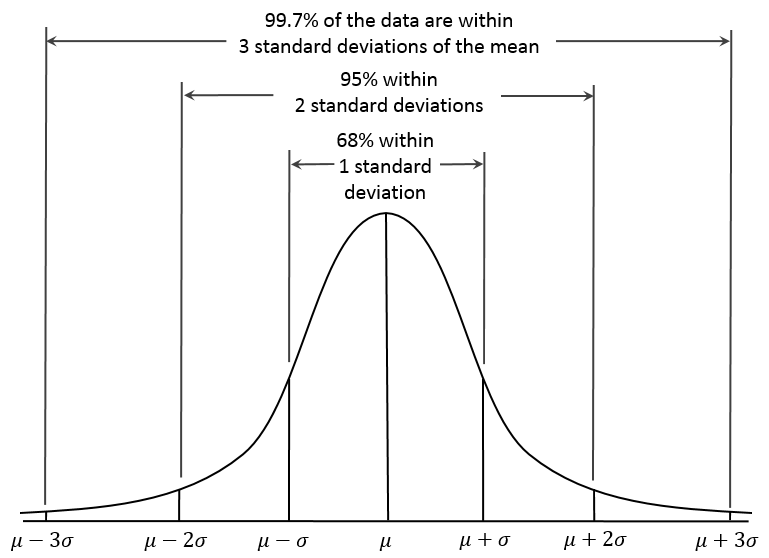
\includegraphics[width=0.9\linewidth]{figures/Empirical_Rule} \caption{The Normal Distribution and the Empirical Rule}\label{fig:EmpRule-fig}
\end{figure}

But if the data are not from an approximately Normal distribution, then this Empirical Rule is less helpful.

\hypertarget{chebyshevs-inequality-one-interpretation-of-the-standard-deviation}{%
\subsection{Chebyshev's Inequality: One Interpretation of the Standard Deviation}\label{chebyshevs-inequality-one-interpretation-of-the-standard-deviation}}

Chebyshev's Inequality tells us that for any distribution, regardless of its relationship to a Normal distribution, no more than 1/k\textsuperscript{2} of the distribution's values can lie more than k standard deviations from the mean. This implies, for instance, that for \textbf{any} distribution, at least 75\% of the values must lie within two standard deviations of the mean, and at least 89\% must lie within three standard deviations of the mean.

Again, most data sets do not follow a Normal distribution. We'll return to this notion soon. But first, let's try to draw some pictures that let us get a better understanding of the distribution of our data.

\hypertarget{measuring-the-shape-of-a-distribution}{%
\section{Measuring the Shape of a Distribution}\label{measuring-the-shape-of-a-distribution}}

When considering the shape of a distribution, one is often interested in three key points.

\begin{itemize}
\tightlist
\item
  The number of modes in the distribution, which I always assess through plotting the data.
\item
  The \textbf{skewness}, or symmetry that is present, which I typically assess by looking at a plot of the distribution of the data, but if required to, will summarise with a non-parametric measure of \textbf{skewness}.
\item
  The \textbf{kurtosis}, or heavy-tailedness (outlier-proneness) that is present, usually in comparison to a Normal distribution. Again, this is something I nearly inevitably assess graphically, but there are measures.
\end{itemize}

A Normal distribution has a single mode, is symmetric and, naturally, is neither heavy-tailed nor light-tailed as compared to a Normal distribution (we call this mesokurtic).

\hypertarget{multimodal-vs.-unimodal-distributions}{%
\subsection{Multimodal vs.~Unimodal distributions}\label{multimodal-vs.-unimodal-distributions}}

A unimodal distribution, on some level, is straightforward. It is a distribution with a single mode, or ``peak'' in the distribution. Such a distribution may be skewed or symmetric, light-tailed or heavy-tailed. We usually describe as multimodal distributions like the two on the right below, which have multiple local maxima, even though they have just a single global maximum peak.

\begin{figure}
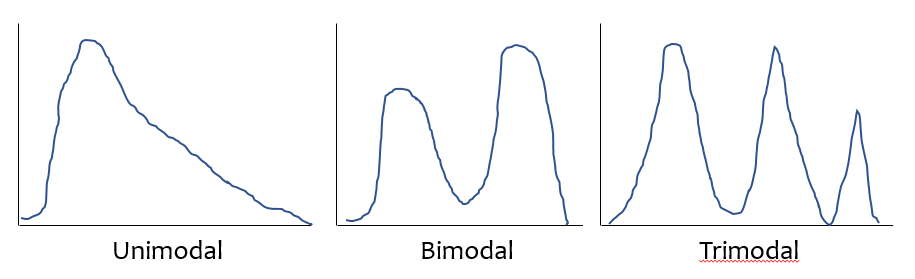
\includegraphics[width=0.9\linewidth]{figures/modality} \caption{Unimodal and Multimodal Sketches}\label{fig:modality-fig}
\end{figure}

Truly multimodal distributions are usually described that way in terms of shape. For unimodal distributions, skewness and kurtosis become useful ideas.

\hypertarget{skew}{%
\subsection{Skew}\label{skew}}

Whether or not a distribution is approximately symmetric is an important consideration in describing its shape. Graphical assessments are always most useful in this setting, particularly for unimodal data. My favorite measure of skew, or skewness if the data have a single mode, is:

\[
skew_1 = \frac{\mbox{mean} - \mbox{median}}{\mbox{standard deviation}}
\]

\begin{itemize}
\tightlist
\item
  Symmetric distributions generally show values of \(skew_1\) near zero. If the distribution is actually symmetric, the mean should be equal to the median.
\item
  Distributions with \(skew_1\) values above 0.2 in absolute value generally indicate meaningful skew.
\item
  Positive skew (mean \textgreater{} median if the data are unimodal) is also referred to as \emph{right skew}.
\item
  Negative skew (mean \textless{} median if the data are unimodal) is referred to as \emph{left skew}.
\end{itemize}

\begin{figure}
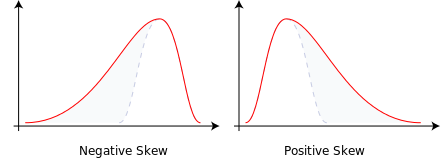
\includegraphics[width=0.9\linewidth]{figures/negandposskew} \caption{Negative (Left) Skew and Positive (Right) Skew}\label{fig:negandposskew-fig}
\end{figure}

\hypertarget{kurtosis}{%
\subsection{Kurtosis}\label{kurtosis}}

When we have a unimodal distribution that is symmetric, we will often be interested in the behavior of the tails of the distribution, as compared to a Normal distribution with the same mean and standard deviation. High values of kurtosis measures (and there are several) indicate data which has extreme outliers, or is heavy-tailed.

\begin{itemize}
\tightlist
\item
  A mesokurtic distribution has similar tail behavior to what we would expect from a Normal distribution.
\item
  A leptokurtic distribution is a thinner distribution, with lighter tails (fewer observations far from the center) than we'd expect from a Normal distribution.
\item
  A platykurtic distribution is a flatter distribution, with heavier tails (more observations far from the center) than we'd expect from a Normal distribution.
\end{itemize}

\begin{figure}
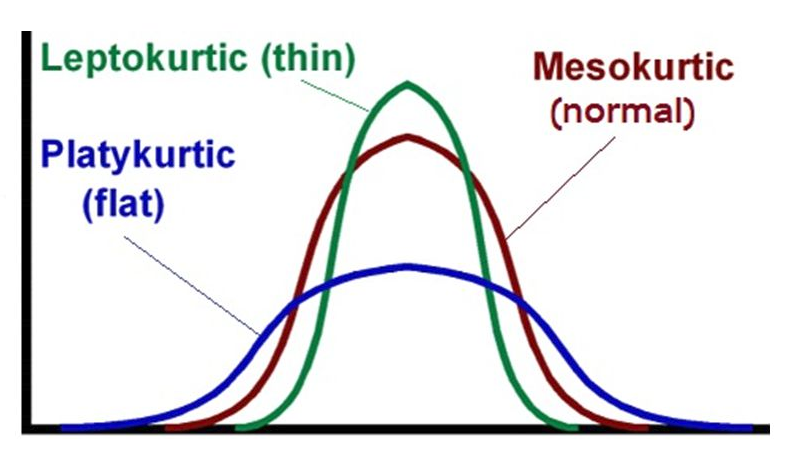
\includegraphics[width=0.9\linewidth]{figures/kurtosis} \caption{The Impact of Kurtosis}\label{fig:kurtosis-fig}
\end{figure}

Graphical tools are in most cases the best way to identify issues related to kurtosis.

\hypertarget{more-detailed-numerical-summaries-for-quantitative-variables}{%
\section{More Detailed Numerical Summaries for Quantitative Variables}\label{more-detailed-numerical-summaries-for-quantitative-variables}}

\hypertarget{favstats-in-the-mosaic-package}{%
\subsection{\texorpdfstring{\texttt{favstats} in the \texttt{mosaic} package}{favstats in the mosaic package}}\label{favstats-in-the-mosaic-package}}

The \texttt{favstats} function adds the standard deviation, and counts of overall and missing observations to our usual \texttt{summary} for a continuous variable. Let's look at systolic blood pressure, because we haven't yet.

\begin{Shaded}
\begin{Highlighting}[]
\NormalTok{mosaic}\OperatorTok{::}\KeywordTok{favstats}\NormalTok{(}\OperatorTok{~}\StringTok{ }\NormalTok{SBP, }\DataTypeTok{data =}\NormalTok{ nh_adults)}
\end{Highlighting}
\end{Shaded}

\begin{verbatim}
 min  Q1 median  Q3 max     mean       sd   n missing
  84 110    118 127 209 119.2495 15.25735 485      15
\end{verbatim}

We could, of course, duplicate these results with a rather lengthy set of \texttt{summarise} pieces\ldots{}

\begin{Shaded}
\begin{Highlighting}[]
\NormalTok{nh_adults }\OperatorTok
\StringTok{    }\KeywordTok{filter}\NormalTok{(}\KeywordTok{complete.cases}\NormalTok{(SBP)) }\OperatorTok
\StringTok{    }\KeywordTok{summarise}\NormalTok{(}\DataTypeTok{min =} \KeywordTok{min}\NormalTok{(SBP), }\DataTypeTok{Q1 =} \KeywordTok{quantile}\NormalTok{(SBP, }\FloatTok{0.25}\NormalTok{), }\DataTypeTok{median =} \KeywordTok{median}\NormalTok{(SBP), }
              \DataTypeTok{Q3 =} \KeywordTok{quantile}\NormalTok{(SBP, }\FloatTok{0.75}\NormalTok{), }\DataTypeTok{max =} \KeywordTok{max}\NormalTok{(SBP),  }
              \DataTypeTok{mean =} \KeywordTok{mean}\NormalTok{(SBP), }\DataTypeTok{sd =} \KeywordTok{sd}\NormalTok{(SBP), }\DataTypeTok{n =} \KeywordTok{n}\NormalTok{(), }\DataTypeTok{missing =} \KeywordTok{sum}\NormalTok{(}\KeywordTok{is.na}\NormalTok{(SBP)))}
\end{Highlighting}
\end{Shaded}

\begin{verbatim}
# A tibble: 1 x 9
    min    Q1 median    Q3   max  mean    sd     n missing
  <int> <dbl>  <int> <dbl> <int> <dbl> <dbl> <int>   <int>
1    84   110    118   127   209  119.  15.3   485       0
\end{verbatim}

The somewhat unusual structure of \texttt{favstats} (complete with an easy to forget \texttt{\textasciitilde{}}) is actually helpful. It allows you to look at some interesting grouping approaches, like this:

\begin{Shaded}
\begin{Highlighting}[]
\NormalTok{mosaic}\OperatorTok{::}\KeywordTok{favstats}\NormalTok{(SBP }\OperatorTok{~}\StringTok{ }\NormalTok{Education, }\DataTypeTok{data =}\NormalTok{ nh_adults)}
\end{Highlighting}
\end{Shaded}

\begin{verbatim}
       Education min  Q1 median     Q3 max     mean       sd   n missing
1      8th Grade  95 114    122 131.50 167 123.7273 18.86085  22       2
2 9 - 11th Grade  92 108    114 125.25 170 117.3833 13.66189  60       0
3    High School  91 112    119 129.00 209 122.6104 19.68111  77       4
4   Some College  85 110    119 128.00 165 119.1812 13.52778 149       4
5   College Grad  84 109    118 126.00 171 117.9209 14.26831 177       5
\end{verbatim}

Of course, we could accomplish the same comparison with \texttt{dplyr} commands, too, but the \texttt{favstats} approach has much to offer.

\begin{Shaded}
\begin{Highlighting}[]
\NormalTok{nh_adults }\OperatorTok
\StringTok{    }\KeywordTok{filter}\NormalTok{(}\KeywordTok{complete.cases}\NormalTok{(SBP, Education)) }\OperatorTok
\StringTok{    }\KeywordTok{group_by}\NormalTok{(Education) }\OperatorTok
\StringTok{    }\KeywordTok{summarise}\NormalTok{(}\DataTypeTok{min =} \KeywordTok{min}\NormalTok{(SBP), }\DataTypeTok{Q1 =} \KeywordTok{quantile}\NormalTok{(SBP, }\FloatTok{0.25}\NormalTok{), }\DataTypeTok{median =} \KeywordTok{median}\NormalTok{(SBP), }
              \DataTypeTok{Q3 =} \KeywordTok{quantile}\NormalTok{(SBP, }\FloatTok{0.75}\NormalTok{), }\DataTypeTok{max =} \KeywordTok{max}\NormalTok{(SBP),  }
              \DataTypeTok{mean =} \KeywordTok{mean}\NormalTok{(SBP), }\DataTypeTok{sd =} \KeywordTok{sd}\NormalTok{(SBP), }\DataTypeTok{n =} \KeywordTok{n}\NormalTok{(), }\DataTypeTok{missing =} \KeywordTok{sum}\NormalTok{(}\KeywordTok{is.na}\NormalTok{(SBP)))}
\end{Highlighting}
\end{Shaded}

\begin{verbatim}
`summarise()` ungrouping output (override with `.groups` argument)
\end{verbatim}

\begin{verbatim}
# A tibble: 5 x 10
  Education        min    Q1 median    Q3   max  mean    sd     n missing
  <fct>          <int> <dbl>  <dbl> <dbl> <int> <dbl> <dbl> <int>   <int>
1 8th Grade         95   114    122  132.   167  124.  18.9    22       0
2 9 - 11th Grade    92   108    114  125.   170  117.  13.7    60       0
3 High School       91   112    119  129    209  123.  19.7    77       0
4 Some College      85   110    119  128    165  119.  13.5   149       0
5 College Grad      84   109    118  126    171  118.  14.3   177       0
\end{verbatim}

\hypertarget{describe-in-the-psych-package}{%
\subsection{\texorpdfstring{\texttt{describe} in the \texttt{psych} package}{describe in the psych package}}\label{describe-in-the-psych-package}}

The \texttt{psych} package has a more detailed list of numerical summaries for quantitative variables that lets us look at a group of observations at once.

\begin{Shaded}
\begin{Highlighting}[]
\NormalTok{psych}\OperatorTok{::}\KeywordTok{describe}\NormalTok{(nh_adults }\OperatorTok\StringTok{ }\KeywordTok{select}\NormalTok{(Age, BMI, SBP, DBP, Pulse))}
\end{Highlighting}
\end{Shaded}

\begin{verbatim}
      vars   n   mean    sd median trimmed   mad  min   max range  skew
Age      1 500  41.91 12.35   42.0   41.86 16.31 21.0  64.0    43  0.03
BMI      2 495  28.48  6.30   27.5   27.80  5.63 17.3  63.3    46  1.35
SBP      3 485 119.25 15.26  118.0  118.25 13.34 84.0 209.0   125  1.27
DBP      4 485  72.13 11.10   72.0   72.33  8.90  0.0 103.0   103 -0.58
Pulse    5 485  73.41 12.01   72.0   73.01 11.86 40.0 112.0    72  0.30
      kurtosis   se
Age      -1.20 0.55
BMI       3.32 0.28
SBP       4.63 0.69
DBP       3.58 0.50
Pulse     0.15 0.55
\end{verbatim}

The additional statistics presented here are:

\begin{itemize}
\tightlist
\item
  \texttt{trimmed} = a trimmed mean (by default in this function, this removes the top and bottom 10\% from the data, then computes the mean of the remaining values - the middle 80\% of the full data set.)
\item
  \texttt{mad} = the median absolute deviation (from the median), which can be used in a manner similar to the standard deviation or IQR to measure spread.

  \begin{itemize}
  \tightlist
  \item
    If the data are \(Y_1, Y_2, ..., Y_n\), then the \texttt{mad} is defined as \(median(|Y_i - median(Y_i)|)\).
  \item
    To find the \texttt{mad} for a set of numbers, find the median, subtract the median from each value and find the absolute value of that difference, and then find the median of those absolute differences.
  \item
    For non-normal data with a skewed shape but tails well approximated by the Normal, the \texttt{mad} is likely to be a better (more robust) estimate of the spread than is the standard deviation.
  \end{itemize}
\item
  a measure of \texttt{skew}, which refers to how much asymmetry is present in the shape of the distribution. The measure is not the same as the \emph{nonparametric skew} measure that we will usually prefer. The {[}Wikipedia page on skewness{]}{[}\url{https://en.wikipedia.org/wiki/Skewness}{]} is very detailed.
\item
  a measure of \texttt{kurtosis}, which refers to how outlier-prone, or heavy-tailed the shape of the distribution is, mainly as compared to a Normal distribution.
\item
  \texttt{se} = the standard error of the sample mean, equal to the sample sd divided by the square root of the sample size.
\end{itemize}

\hypertarget{describe-in-the-hmisc-package}{%
\subsection{\texorpdfstring{\texttt{describe} in the \texttt{Hmisc} package}{describe in the Hmisc package}}\label{describe-in-the-hmisc-package}}

\begin{Shaded}
\begin{Highlighting}[]
\NormalTok{Hmisc}\OperatorTok{::}\KeywordTok{describe}\NormalTok{(nh_adults }\OperatorTok\StringTok{ }\KeywordTok{select}\NormalTok{(Age, BMI, SBP, DBP, Pulse))}
\end{Highlighting}
\end{Shaded}

\begin{verbatim}
nh_adults %>% select(Age, BMI, SBP, DBP, Pulse) 

 5  Variables      500  Observations
--------------------------------------------------------------------------------
Age 
       n  missing distinct     Info     Mean      Gmd      .05      .10 
     500        0       44    0.999    41.91    14.27       23       25 
     .25      .50      .75      .90      .95 
      31       42       53       59       61 

lowest : 21 22 23 24 25, highest: 60 61 62 63 64
--------------------------------------------------------------------------------
BMI 
       n  missing distinct     Info     Mean      Gmd      .05      .10 
     495        5      198        1    28.48    6.704    20.70    21.90 
     .25      .50      .75      .90      .95 
   23.80    27.50    31.60    35.68    41.00 

lowest : 17.3 17.8 18.2 18.3 18.4, highest: 47.7 54.1 54.4 56.8 63.3
--------------------------------------------------------------------------------
SBP 
       n  missing distinct     Info     Mean      Gmd      .05      .10 
     485       15       73    0.999    119.2    16.18       98      102 
     .25      .50      .75      .90      .95 
     110      118      127      137      143 

lowest :  84  85  91  92  93, highest: 170 171 182 202 209
--------------------------------------------------------------------------------
DBP 
       n  missing distinct     Info     Mean      Gmd      .05      .10 
     485       15       61    0.999    72.13    12.02     54.0     58.0 
     .25      .50      .75      .90      .95 
    66.0     72.0     78.0     85.6     89.0 

lowest :   0  41  42  44  45, highest:  98  99 100 102 103
--------------------------------------------------------------------------------
Pulse 
       n  missing distinct     Info     Mean      Gmd      .05      .10 
     485       15       35    0.997    73.41    13.47     54.4     60.0 
     .25      .50      .75      .90      .95 
    64.0     72.0     82.0     88.0     94.0 

lowest :  40  44  48  50  52, highest: 104 106 108 110 112
--------------------------------------------------------------------------------
\end{verbatim}

The \texttt{Hmisc} package's version of \texttt{describe} for a distribution of data presents three new ideas, in addition to a more comprehensive list of quartiles (the 5\textsuperscript{th}, 10\textsuperscript{th}, 25\textsuperscript{th}, 50\textsuperscript{th}, 75\textsuperscript{th}, 90\textsuperscript{th} and 95\textsuperscript{th} are shown) and the lowest and highest few observations. These are:

\begin{itemize}
\tightlist
\item
  \texttt{distinct} - the number of different values observed in the data.
\item
  \texttt{Info} - a measure of how ``continuous'' the variable is, related to how many ``ties'' there are in the data, with Info taking a higher value (closer to its maximum of one) if the data are more continuous.
\item
  \texttt{Gmd} - the Gini mean difference - a robust measure of spread that is calculated as the mean absolute difference between any pairs of observations. Larger values of Gmd indicate more spread-out distributions.
\end{itemize}

\hypertarget{other-options}{%
\subsection{Other options}\label{other-options}}

The package \href{https://cran.r-project.org/web/packages/summarytools/vignettes/Introduction.html}{\texttt{summarytools} has a function called \texttt{dfSummary}} which I like and Dominic Comtois has also published \href{https://cran.r-project.org/web/packages/summarytools/vignettes/Recommendations-rmarkdown.html}{Recommendations for Using summarytools with R Markdown}. Note that this isn't really for Word documents.

The \href{http://naniar.njtierney.com/}{\texttt{naniar} package} is helpful for wrangling and visualizing missing values, and checking imputations.

\href{https://boxuancui.github.io/DataExplorer/}{\texttt{DataExplorer}} can be used for more automated exploratory data analyses (and some people also like \href{https://github.com/ropensci/skimr}{\texttt{skimr}}) and \href{http://visdat.njtierney.com/}{\texttt{visdat}}, as well.

\hypertarget{summarizing-categorical-variables}{%
\chapter{Summarizing Categorical Variables}\label{summarizing-categorical-variables}}

Summarizing categorical variables numerically is mostly about building tables, and calculating percentages or proportions. We'll save our discussion of modeling categorical data for later. Recall that in the \texttt{nh\_adults} data set we built in Section \ref{newNHANES} we had the following categorical variables. The number of levels indicates the number of possible categories for each categorical variable.

\begin{longtable}[]{@{}rlll@{}}
\toprule
Variable & Description & Levels & Type\tabularnewline
\midrule
\endhead
Sex & sex of subject & 2 & binary\tabularnewline
Race & subject's race & 6 & nominal\tabularnewline
Education & subject's educational level & 5 & ordinal\tabularnewline
PhysActive & Participates in sports? & 2 & binary\tabularnewline
Smoke100 & Smoked 100+ cigarettes? & 2 & binary\tabularnewline
SleepTrouble & Trouble sleeping? & 2 & binary\tabularnewline
HealthGen & Self-report health & 5 & ordinal\tabularnewline
\bottomrule
\end{longtable}

\hypertarget{the-summary-function-for-categorical-data}{%
\section{\texorpdfstring{The \texttt{summary} function for Categorical data}{The summary function for Categorical data}}\label{the-summary-function-for-categorical-data}}

When R recognizes a variable as categorical, it stores it as a \emph{factor}. Such variables get special treatment from the \texttt{summary} function, in particular a table of available values (so long as there aren't too many.)

\begin{Shaded}
\begin{Highlighting}[]
\NormalTok{nh_adults }\OperatorTok
\StringTok{  }\KeywordTok{select}\NormalTok{(Sex, Race, Education, PhysActive, Smoke100, }
\NormalTok{         SleepTrouble, HealthGen, MaritalStatus) }\OperatorTok
\StringTok{  }\KeywordTok{summary}\NormalTok{()}
\end{Highlighting}
\end{Shaded}

\begin{verbatim}
     Sex            Race              Education   PhysActive Smoke100 
 female:221   Asian   : 42   8th Grade     : 24   No :215    No :297  
 male  :279   Black   : 63   9 - 11th Grade: 60   Yes:285    Yes:203  
              Hispanic: 26   High School   : 81                       
              Mexican : 38   Some College  :153                       
              White   :313   College Grad  :182                       
              Other   : 18                                            
 SleepTrouble     HealthGen        MaritalStatus
 No :380      Excellent: 50   Divorced    : 51  
 Yes:120      Vgood    :154   LivePartner : 51  
              Good     :184   Married     :259  
              Fair     : 49   NeverMarried:112  
              Poor     : 14   Separated   : 16  
              NA's     : 49   Widowed     : 11  
\end{verbatim}

\hypertarget{tables-to-describe-one-categorical-variable}{%
\section{Tables to describe One Categorical Variable}\label{tables-to-describe-one-categorical-variable}}

Suppose we build a table (using the \texttt{tabyl} function from the \texttt{janitor} package) to describe the \texttt{HealthGen} distribution.

\begin{Shaded}
\begin{Highlighting}[]
\NormalTok{nh_adults }\OperatorTok
\StringTok{    }\KeywordTok{tabyl}\NormalTok{(HealthGen) }\OperatorTok
\StringTok{    }\KeywordTok{adorn_pct_formatting}\NormalTok{()}
\end{Highlighting}
\end{Shaded}

\begin{verbatim}
 HealthGen   n percent valid_percent
 Excellent  50   10.0%         11.1%
     Vgood 154   30.8%         34.1%
      Good 184   36.8%         40.8%
      Fair  49    9.8%         10.9%
      Poor  14    2.8%          3.1%
      <NA>  49    9.8%             -
\end{verbatim}

Note how the missing (\texttt{\textless{}NA\textgreater{}}) values are not included in the \texttt{valid\_percent} calculation, but are in the \texttt{percent} calculation. Note also the use of percentage formatting.

What if we want to add a total count, sometimes called the \emph{marginal} total?

\begin{Shaded}
\begin{Highlighting}[]
\NormalTok{nh_adults }\OperatorTok
\StringTok{    }\KeywordTok{tabyl}\NormalTok{(HealthGen) }\OperatorTok
\StringTok{    }\KeywordTok{adorn_totals}\NormalTok{() }\OperatorTok
\StringTok{    }\KeywordTok{adorn_pct_formatting}\NormalTok{()}
\end{Highlighting}
\end{Shaded}

\begin{verbatim}
 HealthGen   n percent valid_percent
 Excellent  50   10.0%         11.1%
     Vgood 154   30.8%         34.1%
      Good 184   36.8%         40.8%
      Fair  49    9.8%         10.9%
      Poor  14    2.8%          3.1%
      <NA>  49    9.8%             -
     Total 500  100.0%        100.0%
\end{verbatim}

What about marital status, which has no missing data in our sample?

\begin{Shaded}
\begin{Highlighting}[]
\NormalTok{nh_adults }\OperatorTok
\StringTok{    }\KeywordTok{tabyl}\NormalTok{(MaritalStatus) }\OperatorTok
\StringTok{    }\KeywordTok{adorn_totals}\NormalTok{() }\OperatorTok
\StringTok{    }\KeywordTok{adorn_pct_formatting}\NormalTok{()}
\end{Highlighting}
\end{Shaded}

\begin{verbatim}
 MaritalStatus   n percent
      Divorced  51   10.2%
   LivePartner  51   10.2%
       Married 259   51.8%
  NeverMarried 112   22.4%
     Separated  16    3.2%
       Widowed  11    2.2%
         Total 500  100.0%
\end{verbatim}

\hypertarget{the-mode-of-a-categorical-variable}{%
\section{The Mode of a Categorical Variable}\label{the-mode-of-a-categorical-variable}}

A common measure applied to a categorical variable is to identify the mode, the most frequently observed value. To find the mode for variables with lots of categories (so that the \texttt{summary} may not be sufficient), we usually tabulate the data, and then sort by the counts of the numbers of observations, as we did with discrete quantitative variables.

\begin{Shaded}
\begin{Highlighting}[]
\NormalTok{nh_adults }\OperatorTok
\StringTok{    }\KeywordTok{group_by}\NormalTok{(HealthGen) }\OperatorTok
\StringTok{    }\KeywordTok{summarise}\NormalTok{(}\DataTypeTok{count =} \KeywordTok{n}\NormalTok{()) }\OperatorTok
\StringTok{    }\KeywordTok{arrange}\NormalTok{(}\KeywordTok{desc}\NormalTok{(count)) }
\end{Highlighting}
\end{Shaded}

\begin{verbatim}
`summarise()` ungrouping output (override with `.groups` argument)
\end{verbatim}

\begin{verbatim}
# A tibble: 6 x 2
  HealthGen count
  <fct>     <int>
1 Good        184
2 Vgood       154
3 Excellent    50
4 Fair         49
5 <NA>         49
6 Poor         14
\end{verbatim}

\hypertarget{describe-in-the-hmisc-package}{%
\section{\texorpdfstring{\texttt{describe} in the \texttt{Hmisc} package}{describe in the Hmisc package}}\label{describe-in-the-hmisc-package}}

\begin{Shaded}
\begin{Highlighting}[]
\NormalTok{Hmisc}\OperatorTok{::}\KeywordTok{describe}\NormalTok{(nh_adults }\OperatorTok\StringTok{ }
\StringTok{                    }\KeywordTok{select}\NormalTok{(Sex, Race, Education, PhysActive, }
\NormalTok{                           Smoke100, SleepTrouble, }
\NormalTok{                           HealthGen, MaritalStatus))}
\end{Highlighting}
\end{Shaded}

\begin{verbatim}
nh_adults %>% select(Sex, Race, Education, PhysActive, Smoke100, SleepTrouble, HealthGen, MaritalStatus) 

 8  Variables      500  Observations
--------------------------------------------------------------------------------
Sex 
       n  missing distinct 
     500        0        2 
                        
Value      female   male
Frequency     221    279
Proportion  0.442  0.558
--------------------------------------------------------------------------------
Race 
       n  missing distinct 
     500        0        6 

lowest : Asian    Black    Hispanic Mexican  White   
highest: Black    Hispanic Mexican  White    Other   
                                                                
Value         Asian    Black Hispanic  Mexican    White    Other
Frequency        42       63       26       38      313       18
Proportion    0.084    0.126    0.052    0.076    0.626    0.036
--------------------------------------------------------------------------------
Education 
       n  missing distinct 
     500        0        5 

lowest : 8th Grade      9 - 11th Grade High School    Some College   College Grad  
highest: 8th Grade      9 - 11th Grade High School    Some College   College Grad  
                                                                      
Value           8th Grade 9 - 11th Grade    High School   Some College
Frequency              24             60             81            153
Proportion          0.048          0.120          0.162          0.306
                         
Value        College Grad
Frequency             182
Proportion          0.364
--------------------------------------------------------------------------------
PhysActive 
       n  missing distinct 
     500        0        2 
                    
Value        No  Yes
Frequency   215  285
Proportion 0.43 0.57
--------------------------------------------------------------------------------
Smoke100 
       n  missing distinct 
     500        0        2 
                      
Value         No   Yes
Frequency    297   203
Proportion 0.594 0.406
--------------------------------------------------------------------------------
SleepTrouble 
       n  missing distinct 
     500        0        2 
                    
Value        No  Yes
Frequency   380  120
Proportion 0.76 0.24
--------------------------------------------------------------------------------
HealthGen 
       n  missing distinct 
     451       49        5 

lowest : Excellent Vgood     Good      Fair      Poor     
highest: Excellent Vgood     Good      Fair      Poor     
                                                            
Value      Excellent     Vgood      Good      Fair      Poor
Frequency         50       154       184        49        14
Proportion     0.111     0.341     0.408     0.109     0.031
--------------------------------------------------------------------------------
MaritalStatus 
       n  missing distinct 
     500        0        6 

lowest : Divorced     LivePartner  Married      NeverMarried Separated   
highest: LivePartner  Married      NeverMarried Separated    Widowed     
                                                                           
Value          Divorced  LivePartner      Married NeverMarried    Separated
Frequency            51           51          259          112           16
Proportion        0.102        0.102        0.518        0.224        0.032
                       
Value           Widowed
Frequency            11
Proportion        0.022
--------------------------------------------------------------------------------
\end{verbatim}

\hypertarget{cross-tabulations}{%
\section{Cross-Tabulations}\label{cross-tabulations}}

It is very common for us to want to describe the association of one categorical variable with another. For instance, is there a relationship between Education and SleepTrouble in these data?

\begin{Shaded}
\begin{Highlighting}[]
\NormalTok{nh_adults }\OperatorTok
\StringTok{    }\KeywordTok{tabyl}\NormalTok{(Education, SleepTrouble) }\OperatorTok
\StringTok{    }\KeywordTok{adorn_totals}\NormalTok{(}\DataTypeTok{where =} \KeywordTok{c}\NormalTok{(}\StringTok{"row"}\NormalTok{, }\StringTok{"col"}\NormalTok{)) }
\end{Highlighting}
\end{Shaded}

\begin{verbatim}
      Education  No Yes Total
      8th Grade  18   6    24
 9 - 11th Grade  45  15    60
    High School  62  19    81
   Some College 118  35   153
   College Grad 137  45   182
          Total 380 120   500
\end{verbatim}

Note the use of \texttt{adorn\_totals} to get the marginal counts, and how we specify that we want both the row and column totals. We can add a title for the columns with\ldots{}

\begin{Shaded}
\begin{Highlighting}[]
\NormalTok{nh_adults }\OperatorTok
\StringTok{    }\KeywordTok{tabyl}\NormalTok{(Education, SleepTrouble) }\OperatorTok
\StringTok{    }\KeywordTok{adorn_totals}\NormalTok{(}\DataTypeTok{where =} \KeywordTok{c}\NormalTok{(}\StringTok{"row"}\NormalTok{, }\StringTok{"col"}\NormalTok{)) }\OperatorTok
\StringTok{    }\KeywordTok{adorn_title}\NormalTok{(}\DataTypeTok{placement =} \StringTok{"combined"}\NormalTok{)}
\end{Highlighting}
\end{Shaded}

\begin{verbatim}
 Education/SleepTrouble  No Yes Total
              8th Grade  18   6    24
         9 - 11th Grade  45  15    60
            High School  62  19    81
           Some College 118  35   153
           College Grad 137  45   182
                  Total 380 120   500
\end{verbatim}

Often, we'll want to show percentages in a cross-tabulation like this. To get row percentages so that we can directly see the probability of \texttt{SleepTrouble\ =\ Yes} for each level of \texttt{Education}, we can use:

\begin{Shaded}
\begin{Highlighting}[]
\NormalTok{nh_adults }\OperatorTok
\StringTok{    }\KeywordTok{tabyl}\NormalTok{(Education, SleepTrouble) }\OperatorTok
\StringTok{    }\KeywordTok{adorn_totals}\NormalTok{(}\DataTypeTok{where =} \StringTok{"row"}\NormalTok{) }\OperatorTok
\StringTok{    }\KeywordTok{adorn_percentages}\NormalTok{(}\DataTypeTok{denominator =} \StringTok{"row"}\NormalTok{) }\OperatorTok
\StringTok{    }\KeywordTok{adorn_pct_formatting}\NormalTok{() }\OperatorTok
\StringTok{    }\KeywordTok{adorn_title}\NormalTok{(}\DataTypeTok{placement =} \StringTok{"combined"}\NormalTok{)}
\end{Highlighting}
\end{Shaded}

\begin{verbatim}
 Education/SleepTrouble    No   Yes
              8th Grade 75.0% 25.0%
         9 - 11th Grade 75.0% 25.0%
            High School 76.5% 23.5%
           Some College 77.1% 22.9%
           College Grad 75.3% 24.7%
                  Total 76.0% 24.0%
\end{verbatim}

If we want to compare the distribution of \texttt{Education} between the two levels of \texttt{SleepTrouble} with column percentages, we can use the following\ldots{}

\begin{Shaded}
\begin{Highlighting}[]
\NormalTok{nh_adults }\OperatorTok
\StringTok{    }\KeywordTok{tabyl}\NormalTok{(Education, SleepTrouble) }\OperatorTok
\StringTok{    }\KeywordTok{adorn_totals}\NormalTok{(}\DataTypeTok{where =} \StringTok{"col"}\NormalTok{) }\OperatorTok
\StringTok{    }\KeywordTok{adorn_percentages}\NormalTok{(}\DataTypeTok{denominator =} \StringTok{"col"}\NormalTok{) }\OperatorTok
\StringTok{    }\KeywordTok{adorn_pct_formatting}\NormalTok{() }\OperatorTok
\StringTok{    }\KeywordTok{adorn_title}\NormalTok{(}\DataTypeTok{placement =} \StringTok{"combined"}\NormalTok{) }
\end{Highlighting}
\end{Shaded}

\begin{verbatim}
 Education/SleepTrouble    No   Yes Total
              8th Grade  4.7%  5.0%  4.8%
         9 - 11th Grade 11.8% 12.5% 12.0%
            High School 16.3% 15.8% 16.2%
           Some College 31.1% 29.2% 30.6%
           College Grad 36.1% 37.5% 36.4%
\end{verbatim}

If we want overall percentages in the cells of the table, so that the total across all combinations of \texttt{Education} and \texttt{SleepTrouble} is 100\%, we can use:

\begin{Shaded}
\begin{Highlighting}[]
\NormalTok{nh_adults }\OperatorTok
\StringTok{    }\KeywordTok{tabyl}\NormalTok{(Education, SleepTrouble) }\OperatorTok
\StringTok{    }\KeywordTok{adorn_totals}\NormalTok{(}\DataTypeTok{where =} \KeywordTok{c}\NormalTok{(}\StringTok{"row"}\NormalTok{, }\StringTok{"col"}\NormalTok{)) }\OperatorTok
\StringTok{    }\KeywordTok{adorn_percentages}\NormalTok{(}\DataTypeTok{denominator =} \StringTok{"all"}\NormalTok{) }\OperatorTok
\StringTok{    }\KeywordTok{adorn_pct_formatting}\NormalTok{() }\OperatorTok
\StringTok{    }\KeywordTok{adorn_title}\NormalTok{(}\DataTypeTok{placement =} \StringTok{"combined"}\NormalTok{) }
\end{Highlighting}
\end{Shaded}

\begin{verbatim}
 Education/SleepTrouble    No   Yes  Total
              8th Grade  3.6%  1.2%   4.8%
         9 - 11th Grade  9.0%  3.0%  12.0%
            High School 12.4%  3.8%  16.2%
           Some College 23.6%  7.0%  30.6%
           College Grad 27.4%  9.0%  36.4%
                  Total 76.0% 24.0% 100.0%
\end{verbatim}

Another common approach is to include both counts and percentages in a cross-tabulation. Let's look at the breakdown of \texttt{HealthGen} by \texttt{MaritalStatus}.

\begin{Shaded}
\begin{Highlighting}[]
\NormalTok{nh_adults }\OperatorTok
\StringTok{    }\KeywordTok{tabyl}\NormalTok{(MaritalStatus, HealthGen) }\OperatorTok
\StringTok{    }\KeywordTok{adorn_totals}\NormalTok{(}\DataTypeTok{where =} \KeywordTok{c}\NormalTok{(}\StringTok{"row"}\NormalTok{)) }\OperatorTok
\StringTok{    }\KeywordTok{adorn_percentages}\NormalTok{(}\DataTypeTok{denominator =} \StringTok{"row"}\NormalTok{) }\OperatorTok
\StringTok{    }\KeywordTok{adorn_pct_formatting}\NormalTok{() }\OperatorTok
\StringTok{    }\KeywordTok{adorn_ns}\NormalTok{(}\DataTypeTok{position =} \StringTok{"front"}\NormalTok{) }\OperatorTok
\StringTok{    }\KeywordTok{adorn_title}\NormalTok{(}\DataTypeTok{placement =} \StringTok{"combined"}\NormalTok{) }\OperatorTok
\StringTok{    }\NormalTok{knitr}\OperatorTok{::}\KeywordTok{kable}\NormalTok{()}
\end{Highlighting}
\end{Shaded}

\begin{tabular}{l|l|l|l|l|l|l}
\hline
MaritalStatus/HealthGen & Excellent & Vgood & Good & Fair & Poor & NA\_\\
\hline
Divorced & 7 (13.7\%) & 14 (27.5\%) & 20 (39.2\%) & 5  (9.8\%) & 2  (3.9\%) & 3  (5.9\%)\\
\hline
LivePartner & 1  (2.0\%) & 18 (35.3\%) & 16 (31.4\%) & 11 (21.6\%) & 1  (2.0\%) & 4  (7.8\%)\\
\hline
Married & 23  (8.9\%) & 84 (32.4\%) & 102 (39.4\%) & 15  (5.8\%) & 4  (1.5\%) & 31 (12.0\%)\\
\hline
NeverMarried & 14 (12.5\%) & 31 (27.7\%) & 43 (38.4\%) & 13 (11.6\%) & 3  (2.7\%) & 8  (7.1\%)\\
\hline
Separated & 4 (25.0\%) & 4 (25.0\%) & 1  (6.2\%) & 4 (25.0\%) & 1  (6.2\%) & 2 (12.5\%)\\
\hline
Widowed & 1  (9.1\%) & 3 (27.3\%) & 2 (18.2\%) & 1  (9.1\%) & 3 (27.3\%) & 1  (9.1\%)\\
\hline
Total & 50 (10.0\%) & 154 (30.8\%) & 184 (36.8\%) & 49  (9.8\%) & 14  (2.8\%) & 49  (9.8\%)\\
\hline
\end{tabular}

What if we wanted to ignore the missing \texttt{HealthGen} values? Most often, I filter down to the complete observations.

\begin{Shaded}
\begin{Highlighting}[]
\NormalTok{nh_adults }\OperatorTok
\StringTok{    }\KeywordTok{filter}\NormalTok{(}\KeywordTok{complete.cases}\NormalTok{(MaritalStatus, HealthGen)) }\OperatorTok
\StringTok{    }\KeywordTok{tabyl}\NormalTok{(MaritalStatus, HealthGen) }\OperatorTok
\StringTok{    }\KeywordTok{adorn_totals}\NormalTok{(}\DataTypeTok{where =} \KeywordTok{c}\NormalTok{(}\StringTok{"row"}\NormalTok{)) }\OperatorTok
\StringTok{    }\KeywordTok{adorn_percentages}\NormalTok{(}\DataTypeTok{denominator =} \StringTok{"row"}\NormalTok{) }\OperatorTok
\StringTok{    }\KeywordTok{adorn_pct_formatting}\NormalTok{() }\OperatorTok
\StringTok{    }\KeywordTok{adorn_ns}\NormalTok{(}\DataTypeTok{position =} \StringTok{"front"}\NormalTok{) }\OperatorTok
\StringTok{    }\KeywordTok{adorn_title}\NormalTok{(}\DataTypeTok{placement =} \StringTok{"combined"}\NormalTok{)}
\end{Highlighting}
\end{Shaded}

\begin{verbatim}
 MaritalStatus/HealthGen  Excellent       Vgood        Good       Fair
                Divorced  7 (14.6%)  14 (29.2%)  20 (41.7%)  5 (10.4%)
             LivePartner  1  (2.1%)  18 (38.3%)  16 (34.0%) 11 (23.4%)
                 Married 23 (10.1%)  84 (36.8%) 102 (44.7%) 15  (6.6%)
            NeverMarried 14 (13.5%)  31 (29.8%)  43 (41.3%) 13 (12.5%)
               Separated  4 (28.6%)   4 (28.6%)   1  (7.1%)  4 (28.6%)
                 Widowed  1 (10.0%)   3 (30.0%)   2 (20.0%)  1 (10.0%)
                   Total 50 (11.1%) 154 (34.1%) 184 (40.8%) 49 (10.9%)
       Poor
  2  (4.2%)
  1  (2.1%)
  4  (1.8%)
  3  (2.9%)
  1  (7.1%)
  3 (30.0%)
 14  (3.1%)
\end{verbatim}

For more on working with \texttt{tabyls}, see the vignette in the \texttt{janitor} package. There you'll find a complete list of all of the \texttt{adorn} functions, for example.

Here's another approach, to look at the cross-classification of Race and HealthGen:

\begin{Shaded}
\begin{Highlighting}[]
\KeywordTok{xtabs}\NormalTok{(}\OperatorTok{~}\StringTok{ }\NormalTok{Race }\OperatorTok{+}\StringTok{ }\NormalTok{HealthGen, }\DataTypeTok{data =}\NormalTok{ nh_adults)}
\end{Highlighting}
\end{Shaded}

\begin{verbatim}
          HealthGen
Race       Excellent Vgood Good Fair Poor
  Asian            3    11   17    3    0
  Black            8    11   19   11    6
  Hispanic         3     3   11    4    1
  Mexican          2     8   17    6    3
  White           33   113  114   22    4
  Other            1     8    6    3    0
\end{verbatim}

\hypertarget{cross-classifying-three-categorical-variables}{%
\subsection{Cross-Classifying Three Categorical Variables}\label{cross-classifying-three-categorical-variables}}

Suppose we are interested in \texttt{Smoke100} and its relationship to \texttt{PhysActive} and \texttt{SleepTrouble}.

\begin{Shaded}
\begin{Highlighting}[]
\NormalTok{nh_adults }\OperatorTok
\StringTok{    }\KeywordTok{tabyl}\NormalTok{(Smoke100, PhysActive, SleepTrouble) }\OperatorTok
\StringTok{    }\KeywordTok{adorn_title}\NormalTok{(}\DataTypeTok{placement =} \StringTok{"top"}\NormalTok{)}
\end{Highlighting}
\end{Shaded}

\begin{verbatim}
$No
          PhysActive    
 Smoke100         No Yes
       No         99 142
      Yes         62  77

$Yes
          PhysActive    
 Smoke100         No Yes
       No         21  35
      Yes         33  31
\end{verbatim}

The result here is a tabyl of \texttt{Smoke100} (rows) by \texttt{PhysActive} (columns), split into a list by \texttt{SleepTrouble}. Another approach to get the same table is:

\begin{Shaded}
\begin{Highlighting}[]
\KeywordTok{xtabs}\NormalTok{(}\OperatorTok{~}\StringTok{ }\NormalTok{Smoke100 }\OperatorTok{+}\StringTok{ }\NormalTok{PhysActive }\OperatorTok{+}\StringTok{ }\NormalTok{SleepTrouble, }\DataTypeTok{data =}\NormalTok{ nh_adults)}
\end{Highlighting}
\end{Shaded}

\begin{verbatim}
, , SleepTrouble = No

        PhysActive
Smoke100  No Yes
     No   99 142
     Yes  62  77

, , SleepTrouble = Yes

        PhysActive
Smoke100  No Yes
     No   21  35
     Yes  33  31
\end{verbatim}

We can also build a \textbf{flat} version of this table, as follows:

\begin{Shaded}
\begin{Highlighting}[]
\KeywordTok{ftable}\NormalTok{(Smoke100 }\OperatorTok{~}\StringTok{ }\NormalTok{PhysActive }\OperatorTok{+}\StringTok{ }\NormalTok{SleepTrouble, }\DataTypeTok{data =}\NormalTok{ nh_adults)}
\end{Highlighting}
\end{Shaded}

\begin{verbatim}
                        Smoke100  No Yes
PhysActive SleepTrouble                 
No         No                     99  62
           Yes                    21  33
Yes        No                    142  77
           Yes                    35  31
\end{verbatim}

And we can do this with \texttt{dplyr} functions, as well, for example\ldots{}

\begin{Shaded}
\begin{Highlighting}[]
\NormalTok{nh_adults }\OperatorTok
\StringTok{    }\KeywordTok{select}\NormalTok{(Smoke100, PhysActive, SleepTrouble) }\OperatorTok
\StringTok{    }\KeywordTok{table}\NormalTok{() }
\end{Highlighting}
\end{Shaded}

\begin{verbatim}
, , SleepTrouble = No

        PhysActive
Smoke100  No Yes
     No   99 142
     Yes  62  77

, , SleepTrouble = Yes

        PhysActive
Smoke100  No Yes
     No   21  35
     Yes  33  31
\end{verbatim}

\hypertarget{constructing-tables-well}{%
\section{Constructing Tables Well}\label{constructing-tables-well}}

The prolific Howard Wainer is responsible for many interesting books on visualization and related issues, including \citet{HW_GraphicDiscovery} and \citet{HW_MedicalIlluminations}. These rules come from Chapter 10 of \citet{HW_VisualRevelations}.

\begin{enumerate}
\def\labelenumi{\arabic{enumi}.}
\tightlist
\item
  Order the rows and columns in a way that makes sense.
\item
  Round, a lot!
\item
  ALL is different and important
\end{enumerate}

\hypertarget{alabama-first}{%
\subsection{Alabama First!}\label{alabama-first}}

Which of these Tables is more useful to you?

2013 Percent of Students in grades 9-12 who are obese

\begin{longtable}[]{@{}lccc@{}}
\toprule
State & \% Obese & 95\% CI & Sample Size\tabularnewline
\midrule
\endhead
Alabama & 17.1 & (14.6 - 19.9) & 1,499\tabularnewline
Alaska & 12.4 & (10.5-14.6) \textbar{} 1, & 1,167\tabularnewline
Arizona & 10.7 \textbar{} (8.3 & (8.3-13.6) \textbar{} 1,52 & 1,520\tabularnewline
Arkansas & 17.8 \textbar{} (15.7- & (15.7-20.1) \textbar{} & 1,470\tabularnewline
Connecticut & 12.3 \textbar{} & (10.2-14.7) \textbar{} 2,2 & 2,270\tabularnewline
Delaware & 14.2 \textbar{} (12 & (12.9-15.6) \textbar{} & 2,475\tabularnewline
Florida & 11.6 \textbar{} (10.5-1 & (10.5-12.8) \textbar{} & 5,491\tabularnewline
\ldots{} & & &\tabularnewline
Wisconsin & 11.6 \textbar{} ( & (9.7-13.9) \textbar{} 2,7 & 2,771\tabularnewline
Wyoming & 10.7 & (9.4-12.2) \textbar{} 2,910 & 2,910\tabularnewline
\bottomrule
\end{longtable}

or \ldots{}

\begin{longtable}[]{@{}lccc@{}}
\toprule
State & \% Obese & 95\% CI & Sample Size\tabularnewline
\midrule
\endhead
Kentucky & 18.0 & (15.7 - 20.6) & 1,537\tabularnewline
Arkansas & 17.8 & (15.7 - 20.1) & 1,470\tabularnewline
Alabama & 17.1 & (14.6 - 19.9) & 1,499\tabularnewline
Tennessee & 16.9 & (15.1 - 18.8) & 1,831\tabularnewline
Texas & 15.7 & (13.9 - 17.6) & 3,039\tabularnewline
\ldots{} & & &\tabularnewline
Massachusetts & 10.2 & (8.5 - 12.1) & 2,547\tabularnewline
Idaho & 9.6 & (8.2 - 11.1) & 1,841\tabularnewline
Montana & 9.4 & (8.4 - 10.5) & 4,679\tabularnewline
New Jersey & 8.7 & (6.8 - 11.2) & 1,644\tabularnewline
Utah & 6.4 & (4.8 - 8.5) & 2,136\tabularnewline
\bottomrule
\end{longtable}

It is a rare event when Alabama first is the best choice.

\hypertarget{order-rows-and-columns-sensibly}{%
\subsection{Order rows and columns sensibly}\label{order-rows-and-columns-sensibly}}

\begin{itemize}
\tightlist
\item
  Alabama First!

  \begin{itemize}
  \tightlist
  \item
    Size places - put the largest first. We often look most carefully at the top.
  \end{itemize}
\item
  Order time from the past to the future to help the viewer.
\item
  If there is a clear predictor-outcome relationship, put the predictors in the rows and the outcomes in the columns.
\end{itemize}

\hypertarget{round---a-lot}{%
\subsection{Round - a lot!}\label{round---a-lot}}

\begin{itemize}
\tightlist
\item
  Humans cannot understand more than two digits very easily.
\item
  We almost never care about accuracy of more than two digits.
\item
  We can almost never justify more than two digits of accuracy statistically.
\item
  It's also helpful to remember that we are almost invariably publishing progress to date, rather than a truly final answer.
\end{itemize}

Suppose, for instance, we report a correlation coefficient of 0.25. How many observations do you think you would need to justify such a choice?

\begin{itemize}
\tightlist
\item
  To report 0.25 meaningfully, we want to be sure that the second digit isn't 4 or 6.
\item
  That requires a standard error less than 0.005
\item
  The \emph{standard error} of any statistic is proportional to 1 over the square root of the sample size, \emph{n}.
\end{itemize}

So \(\frac{1}{\sqrt{n}}\) \textasciitilde{} 0.005, but that means \(\sqrt{n} = \frac{1}{0.005} = 200\). If \(\sqrt{n} = 200\), then \emph{n} = (200)\textsuperscript{2} = 40,000.

Do we usually have 40,000 observations?

\hypertarget{all-is-different-and-important}{%
\subsection{ALL is different and important}\label{all-is-different-and-important}}

Summaries of rows and columns provide a measure of what is typical or usual. Sometimes a sum is helpful, at other times, consider presenting a median or other summary. The ALL category, as \citet{HW_VisualRevelations} suggests, should be both visually different from the individual entries and set spatially apart.

On the whole, it's \emph{far} easier to fall into a good graph in R (at least if you have some ggplot2 skills) than to produce a good table.

\hypertarget{gaining-control-over-tables-in-r-the-gt-package}{%
\section{\texorpdfstring{Gaining Control over Tables in R: the \texttt{gt} package}{Gaining Control over Tables in R: the gt package}}\label{gaining-control-over-tables-in-r-the-gt-package}}

With the \texttt{gt} package, anyone can make wonderful-looking tables using the R programming language. The \texttt{gt} package is described in substantial detail at \url{https://gt.rstudio.com/} and we'll get started with it soon.

  \bibliography{book.bib,packages.bib}

\end{document}
